\documentclass{article}

% if you need to pass options to natbib, use, e.g.:
%     \PassOptionsToPackage{numbers, compress}{natbib}
% before loading neurips_2026

% The authors should use one of these tracks.
% Before accepting by the NeurIPS conference, select one of the options below.
% 0. "default" for submission
% \usepackage{neurips_2026}
% the "default" option is equal to the "main" option, which is used for the Main Track with double-blind reviewing.
% 1. "main" option is used for the Main Track
%  \usepackage[main]{neurips_2026}
% 2. "position" option is used for the Position Paper Track
%  \usepackage[position]{neurips_2026}
% 3. "eandd" option is used for the Evaluations & Datasets Track
 % \usepackage[eandd]{neurips_2026}
% 4. "creativeai" option is used for the Creative AI Track
%  \usepackage[creativeai]{neurips_2026}
% 5. "sglblindworkshop" option is used for the Workshop with single-blind reviewing
 % \usepackage[sglblindworkshop]{neurips_2026}
% 6. "dblblindworkshop" option is used for the Workshop with double-blind reviewing
%  \usepackage[dblblindworkshop]{neurips_2026}
% 7. "education" option is used for the Education Track
%  \usepackage[education]{neurips_2026}


% After being accepted, the authors should add "final" behind the track to compile a camera-ready version.
% 1. Main Track
\usepackage[main, final]{neurips_2026}
% 2. Position Paper Track
%  \usepackage[position, final]{neurips_2026}
% 3. Evaluations & Datasets Track
 % \usepackage[eandd, final]{neurips_2026}
% 4. Creative AI Track
%  \usepackage[creativeai, final]{neurips_2026}
% 5. Workshop with single-blind reviewing
%  \usepackage[sglblindworkshop, final]{neurips_2026}
% 6. Workshop with double-blind reviewing
%  \usepackage[dblblindworkshop, final]{neurips_2026}
% Note. For the workshop paper template, both \title{} and \workshoptitle{} are required, with the former indicating the paper title shown in the title and the latter indicating the workshop title displayed in the footnote.
% For workshops (5., 6.), the authors should add the name of the workshop, "\workshoptitle" command is used to set the workshop title.
% \workshoptitle{WORKSHOP TITLE}
% 7. Education Track
% \usepackage[education, final]{neurips_2026}

% "preprint" option is used for arXiv or other preprint submissions
 % \usepackage[preprint]{neurips_2026}

% to avoid loading the natbib package, add option nonatbib:
%    \usepackage[nonatbib]{neurips_2026}

% xcolor is first loaded below without options; pass the options the paper loads it with
% (\usepackage[dvipsnames,table]{xcolor} further down) so the two loads do not clash.
\PassOptionsToPackage{dvipsnames,table}{xcolor}

\usepackage[utf8]{inputenc} % allow utf-8 input
\usepackage[T1]{fontenc}    % use 8-bit T1 fonts
\usepackage{hyperref}       % hyperlinks
\usepackage{url}            % simple URL typesetting
\usepackage{booktabs}       % professional-quality tables
\usepackage{amsfonts}       % blackboard math symbols
\usepackage{nicefrac}       % compact symbols for 1/2, etc.
\usepackage{microtype}      % microtypography
\usepackage{xcolor}         % colors

% --- Layout & Geometry ---
% (geometry, titlesec, authblk not loaded: they clash with or override the page layout, headings and author block of neurips_2026)
\usepackage{indentfirst}
\usepackage{fancyhdr}

% --- Language & Fonts ---
\usepackage[utf8]{inputenc}
\usepackage[T1]{fontenc}
\usepackage{microtype}
\usepackage{xspace}

% --- Math Packages ---
\usepackage{amsmath}
\usepackage{amssymb}
\usepackage{amsthm}
\usepackage{amsfonts}
\usepackage{mathtools}
\usepackage{bbm}
% bbm has only bitmap (Type 3) fonts, which NeurIPS does not accept; typeset \mathbbm with the Type 1 dsfont glyphs
\usepackage{dsfont}
\renewcommand{\mathbbm}[1]{\mathds{#1}}
\usepackage{bm}
\usepackage{nicefrac}

% --- Colors (loaded with global options up front to prevent clashes) ---
\usepackage[dvipsnames,table]{xcolor}
\definecolor{burgundy}{rgb}{0.5, 0.0, 0.13}
\definecolor{antiquewhite}{rgb}{0.98, 0.92, 0.84}
\definecolor{blizzardblue}{rgb}{0.67, 0.9, 0.93}
\colorlet{shadecolor}{pink}
\definecolor{lightpurple}{RGB}{225, 215, 245}
\definecolor{cobrasblue}{RGB}{235, 242, 250}

% --- Graphics, Figures & Captions ---
\usepackage{graphicx}
\usepackage{subcaption}
\usepackage{wrapfig}
\usepackage{framed}
\usepackage{soul}
\usepackage{pifont}
\newcommand{\cmark}{\ding{51}}%
\newcommand{\xmark}{\ding{55}}%
\usepackage{caption}

% --- Tables & Lists ---
\usepackage{booktabs}
\usepackage{multirow}
\usepackage{makecell}
\usepackage{adjustbox}
\usepackage{threeparttable}
\usepackage{tablefootnote}
\usepackage{siunitx}
\usepackage{paralist}
\usepackage{colortbl}
\usepackage{longtable}
\usepackage[shortlabels]{enumitem}

% --- Algorithms ---
\usepackage{algorithm}
\usepackage{algpseudocode}
\newcommand{\algcolor}[3]{\hspace*{-\fboxsep}\colorbox{#1}{\parbox{#2\linewidth}{#3}}}

% --- Boxes & Floats ---
\usepackage[most]{tcolorbox}
\tcbuselibrary{breakable}
\usepackage{placeins}

% Avoid stacking figures and keep float-only pages aligned at the top.
\setcounter{topnumber}{1}
\makeatletter
\setlength{\@fptop}{0pt}
\setlength{\@dblfptop}{0pt}
\makeatother

% --- Bibliographies & Citations ---
\usepackage{natbib}
\usepackage{doi}

% --- Miscellaneous ---
\usepackage{comment}
\usepackage{csquotes}
\usepackage[colorinlistoftodos,bordercolor=orange,backgroundcolor=orange!20,linecolor=orange,textsize=scriptsize]{todonotes}

% --- Hyperlinks & Cross-Referencing (loaded last) ---
\usepackage{hyperref}
\usepackage{url}
\usepackage{cleveref}

\hypersetup{
    colorlinks=true,
    citecolor=burgundy,
    linkcolor=blue,
    filecolor=magenta,
    urlcolor=cyan
}
\urlstyle{same}

% --- Theorem Environments ---
\theoremstyle{plain}
\newtheorem{theorem}{Theorem}
\newtheorem{proposition}[theorem]{Proposition}
\newtheorem{lemma}[theorem]{Lemma}
\newtheorem{corollary}[theorem]{Corollary}
\newtheorem{definition}[theorem]{Definition}
\newtheorem{example}[theorem]{Example}
\newtheorem{conjecture}[theorem]{Conjecture}
\newtheorem{assumption}[theorem]{Assumption}
\newtheorem{hypothesis}[theorem]{Hypothesis}
\newtheorem{remark}[theorem]{Remark}
\newtheorem{fact}[theorem]{Fact}

% --- Custom Math Commands ---
\newcommand{\vertiii}[1]{{\left\vert\kern-0.25ex\left\vert\kern-0.25ex\left\vert #1
  \right\vert\kern-0.25ex\right\vert\kern-0.25ex\right\vert}}



\newcommand{\pzero}{p_{0}}
\newcommand{\pplus}{p_{+}}
\newcommand{\pplushat}{\hat{p}_{+}}
\newcommand{\pminus}{p_{-}}
\newcommand{\pminushat}{\hat{p}_{-}}
\newcommand{\Pref}{\mathbb{P}}
\newcommand{\Qstar}{\mathbb{Q}^{\star}}
\newcommand{\Sph}{\mathcal{S}}
\newcommand{\KL}{\mathrm{KL}}
\newcommand{\Law}{\mathrm{Law}}
\newcommand{\nablaS}{\nabla_{\Sph}}
\newcommand{\Lzero}{\mathcal{L}^{0}}
\newcommand{\kzero}{k_{T}^{\pzero}}
\newcommand{\hquery}{\boldsymbol{h}_{q}}
\newcommand{\Cobras}{\textsc{Cobras}\xspace}
\newcommand{\etal}{\textit{et al.}}

% Note. For the workshop paper template, both \title{} and \workshoptitle{} are required, with the former indicating the paper title shown in the title and the latter indicating the workshop title displayed in the footnote. 
\title{Conditional Optimal Bridge for Riemannian Activation Steering}


% The \author macro works with any number of authors. There are two commands
% used to separate the names and addresses of multiple authors: \And and \AND.
%
% Using \And between authors leaves it to LaTeX to determine where to break the
% lines. Using \AND forces a line break at that point. So, if LaTeX puts 3 of 4
% authors names on the first line, and the last on the second line, try using
% \AND instead of \And before the third author name.


\author{%
  Seyed Arshan Dalili \\
  The Pennsylvania State University \\
  University Park, PA 16802 \\
  \texttt{sbd5760@psu.edu} \\
  \And
  Ajay Narayanan Sridhar \\
  Georgia Institute of Technology \\
  Atlanta, GA 30332 \\
  \texttt{afs6372@psu.edu} \\
  \AND
  Vijaykrishnan Narayanan \\
  Georgia Institute of Technology \\
  Atlanta, GA 30332 \\
  \texttt{vxn9@psu.edu} \\
  \And
  Mehrdad Mahdavi \\
  The Pennsylvania State University \\
  University Park, PA 16802 \\
  \texttt{mzm616@psu.edu} \\
}


\begin{document}
\maketitle


\begin{abstract}
Activation steering offers a lightweight alternative to fine-tuning for controlling large language models at inference time. \textcolor{blue}{Many existing methods implicitly optimize a log-density-ratio objective between desired and undesired activation distributions without a principled derivation. Fixed steering directions can also degrade in-distribution and out-of-distribution (OOD) performance. We introduce \textsc{Cobras} (Conditional Optimal Bridge for Riemannian Activation Steering), which casts steering as a Schr\"{o}dinger Bridge on the residual-stream hypersphere.} This formulation yields, to our knowledge, the first principled derivation of the log-density-ratio steering objective from a well-posed optimization problem. \textcolor{blue}{We use entropic optimal transport to construct a query-adaptive steering field that recovers log-density-ratio steering as a limiting case. The fitted transport also provides a support score for controlling OOD interventions. Across four models, \textsc{Cobras} outperforms prior steering methods in nearly all model--task settings spanning helpfulness, truthfulness, and detoxification, while largely preserving OOD performance. Code is available \href{https://github.com/arshandalili/cobras}{here}.}
\end{abstract}


\bigskip

\section{Introduction}
Activation steering has emerged as a compelling alternative to fine-tuning for shaping the behavior of large language models (LLMs) at inference time \citep{rimsky2024steering, li2023inference, wang2025truthflow}. Its empirical success is often motivated by the linear representation hypothesis \citep{park2023linear, alain2016understanding}, where many high-level properties encoded by an LLM, such as sentiment, truthfulness, or harmfulness, appear to correspond to approximately linear directions in activation space. Under this view, changing a model's behavior can be achieved by moving its internal activations along directions associated with the target property at inference time. A standard approach is activation addition, which modifies the original activations by adding either a fixed steering vector or one that depends on the current activation.

This perspective has inspired a growing body of work on inference-time control through activation interventions. Early methods typically construct a single steering direction from contrastive examples and then apply that direction uniformly across queries \citep{rimsky2024steering}, while more recent approaches refine the dynamics of the intervention by integrating a continuous steering field over multiple steps \citep{zhaoodesteer, wang2025truthflow, rodriguez2025controlling} or working on a more faithful manifold by rotating activations on the hypersphere \cite{you2026spherical, pham2024householder}. 
\noindent~Despite this progress, existing methods share two limitations. First, most of the methods and their implicit objective are heuristic rather than \emph{derived} from a well-posed optimization problem without formal justification for the objective itself. Second, these steering signals are \emph{query-independent}. A steering vector that helps in-distribution prompts can make out-of-distribution (OOD) inputs wrong or gibberish, and our experiments confirm that several strong baselines improve TruthfulQA~\cite{lin2021truthfulqa} at the cost of severe MMLU~\cite{hendrycks2020measuring} and GSM8K~\cite{cobbe2021gsm8k} degradation. We address both gaps with \Cobras, which casts steering as a Schr\"{o}dinger Bridge, yielding both a principled \emph{derivation} of the steering objective and an inherently query-adaptive steering direction, along with its OOD capability.

Overall, our contributions are: (i) we show that the Schr\"{o}dinger Bridge on the activation hypersphere provides a principled derivation of the implicitly widely used log-density-ratio steering objective; (ii) we propose Conditional Optimal Bridge for Riemannian Activation Steering (\Cobras), a practical algorithm that combines entropic optimal-transport potentials and an inherent gating mechanism to produce query-adaptive steering directions; and (iii) we demonstrate that \Cobras consistently outperforms prior baselines on helpfulness, truthfulness, and detoxification while avoiding the out-of-distribution degradation observed in existing methods.


\paragraph{Organization.}Section~\ref{sec:related} discusses the related work. Section~\ref{sec:bg} elaborates on the background, notation, setup, and the assumption of the manifold where LLM activations exist. Section~\ref{sec:method} then formulates the steering problem and its objective as the Schr\"{o}dinger Bridge instance, solves this problem, derives the objective for steering, and proposes \Cobras. Section~\ref{sec:exp} then does extensive experiments for both in-distribution and OOD and shows that \Cobras outperforms baselines in both settings. Finally, Section~\ref{sec:conclusion} concludes the paper, discussing limitations and future work. The proof of technical results and additional experiments are reported in the appendix. 



\vspace{-1mm}
\section{Related Work}
\label{sec:related}
\noindent\textbf{Theory of activation steering.}~Several recent works have sought to develop a unified theory of activation steering by interpreting interventions as structured transformations in representation space. Linear Activation Transportation~\citep{rodriguez2025controlling} formulates steering as a transport map between source and target activation distributions, LiSeCo~\citep{cheng2024linearly} analyzes steering through linear separability and constrained optimization, and ODESteer~\citep{zhaoodesteer} views steering as a continuous-time dynamical process rather than a one-shot activation edit. \citet{taimeskhanov2026towards} theoretically study the effect of steering strength in additive interventions, characterizing its impact on next-token probabilities, concept expression, and cross-entropy. These perspectives provide useful formal tools for reasoning about activation interventions. These perspectives provide useful formal tools for reasoning about activation interventions. However, their guarantees are typically derived for surrogate objectives and under specific geometric constraints rather than from a principled perspective. Also, the Schr\"odinger Bridge (SB) problem has been widely adopted for generative modeling via forward--backward SDE solvers~\citep{de2021diffusion, chen2021likelihood, shi2023diffusion}. \Cobras is the first to apply this
framework for LLM activation steering.

\noindent\textbf{Activation steering approaches.}~Early and widely used steering approaches~\cite{zou2023representation, li2023inference, rimsky2024steering} identify behavior-relevant directions in activation space and apply additive edits. More recent methods refine this basic recipe by accounting for activation geometry or distributional structure, for example through minimally invasive affine maps~\citep{singh2024representation}, norm-preserving rotations~\citep{pham2024householder}, transport-based maps~\citep{rodriguez2025controlling}, hyperspherical interventions~\citep{you2026spherical}, or continuous dynamical updates~\citep{zhaoodesteer}. Despite these advances, most existing methods are query-independent: once a direction or transformation is learned, essentially the same intervention is applied across prompts. Prior work shows that such fixed interventions can have limited OOD generalization, induce off-target side effects, and degrade performance when steering is unnecessary~\citep{tan2024analysing,raedler2025necessity,da2025steering}. Our work instead proposes a query-adaptive steering method that modulates the intervention based on the input, preserving OOD performance while improving in-distribution performance.
 

% Representation Engineering (RepE)~\citep{zou2023representation} showed that high-level concepts and behaviors can often be represented as directions in hidden-state/activation space, enabling direct manipulation of model representations. Building on this idea, Inference-Time Intervention (ITI)~\citep{li2023inference} steers selected attention-head activations along truthfulness-related directions, while Contrastive Activation Addition (CAA)~\citep{rimsky2024steering} constructs steering vectors from differences between positive and negative examples and adds them to residual-stream activations during generation. More recent methods move beyond simple additive interventions by considering richer activation geometry and distributional structure: Minimally Modified Counterfactuals (MiMiC)~\citep{singh2024representation} applies minimally invasive affine transformations to match counterfactual activation statistics, Householder Pseudo-Rotation (HPR)~\citep{pham2024householder} uses norm-preserving pseudo-rotations, Linear Activation Transport (Linear-AcT)~\citep{rodriguez2025controlling} formulates steering as a transport map between source and target activation distributions, SphericalSteering~\citep{you2026spherical} performs steering on the hypersphere to preserve activation magnitudes, and ODESteer~\citep{zhaoodesteer} interprets steering as a continuous dynamical process rather than a one-shot edit.

% Most of the present steering methods, are query indepdent, they end up steering using a constant steering direction which leads to catastrophic failure of performance in OOD tasks. In our work, we propose a query adaptive steering method that retains it performacne in OOD tasks while improving perofrmance on in-diostribution tasks. 

% Query indepdent ; Cobras is query adaptive ; see some failure cases; \textcolor{blue}{AD: mention catastrophic performance of OOD as the result of not being query-adaptive} 

\section{Background}
\label{sec:bg}

\paragraph{Setup and notation.}
We fix a decoder-only transformer of residual width $d$ and a layer index $\ell$, and write
$\boldsymbol{h}\in\mathbb{R}^{d}$ for the layer-$\ell$ residual-stream activation at the last token position.
Two populations of inputs are given, one exhibiting a desired behavior and one an undesired behavior, with
activation distributions $\pplus$ and $\pminus$ observed through i.i.d.\ samples
$\mathcal{D}^{+}=\{\boldsymbol{h}^{+}_{i}\}_{i=1}^{N_{+}}\sim\pplus$ and
$\mathcal{D}^{-}=\{\boldsymbol{h}^{-}_{j}\}_{j=1}^{N_{-}}\sim\pminus$, whose empirical measures we denote
$\pplushat$ and $\pminushat$. At inference, a steering map is applied to the layer-$\ell$ activation of each
decoded token, beginning with the last prompt token, and $\hquery$ denotes the activation currently being
steered. The map should move $\hquery$ toward regions of high density under $\pplus$ and low density under
$\pminus$, and it modifies no other activation. Vectors and vector fields are set in bold.

\paragraph{Spherical geometry of activations.}
Residual-stream norms concentrate tightly across inputs at a fixed layer, both
empirically~\citep{pham2024householder, you2026spherical} and as a consequence of the residual
architecture~\citep{yang2023spectral, xie2026controlled}. Figure~\ref{fig:norm-concentration} shows this
for the four models we study, for which the coefficient of variation of the layer-normalized last-token norm
lies between $2.5\%$ and $7.3\%$, and Appendix~\ref{appendix:norm_concentration} reports the same
measurement layer by layer and for four further architectures. We therefore model the state space as the
sphere $\Sph=\{\boldsymbol{x}\in\mathbb{R}^{d}:\lVert\boldsymbol{x}\rVert=R\}$ of radius $R$, the mean norm
over $\mathcal{D}^{+}\cup\mathcal{D}^{-}$, and restore the original norm of $\hquery$ after steering, so that
the intervention changes only the direction of the activation.

\begin{figure}[!ht]
\centering
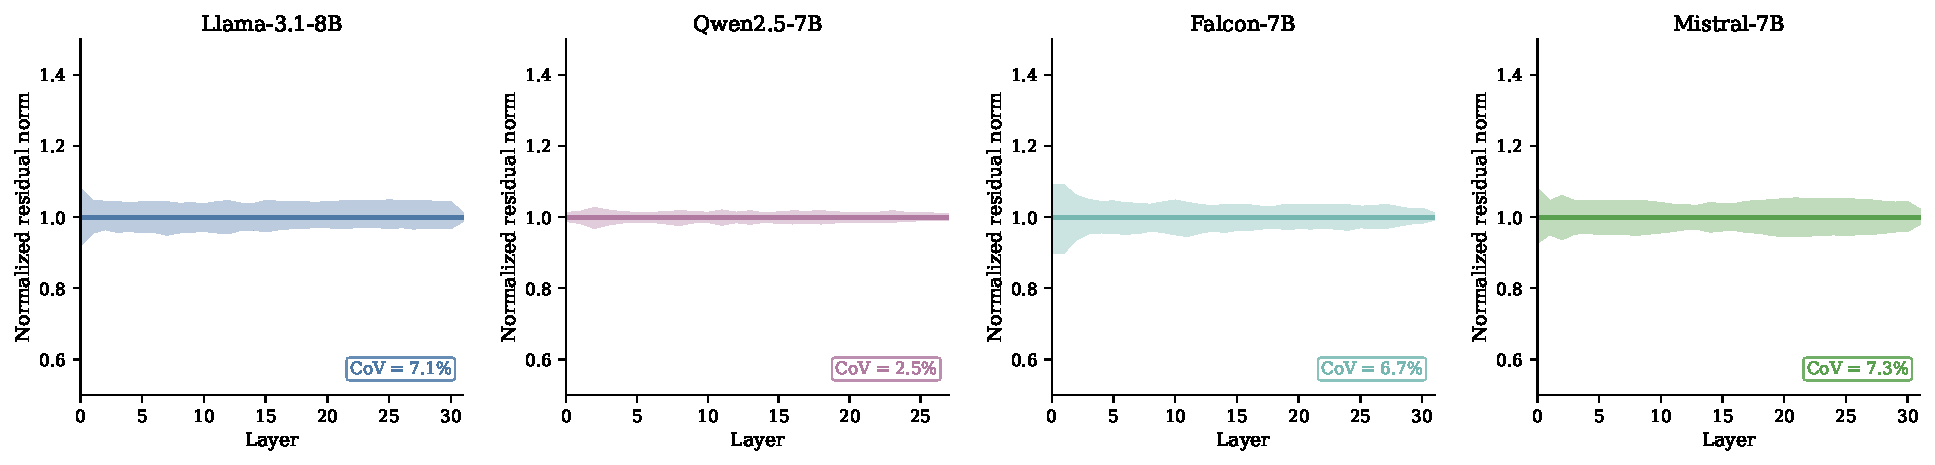
\includegraphics[width=\textwidth]{figures/norm_concentration.pdf}
\caption{Last-token residual-stream norms across layers on TruthfulQA for four LLMs, each divided by its
layer-wise mean. Dark and light bands show the 25th--75th percentiles. The coefficient of variation (CoV) is
reported per model.}
\label{fig:norm-concentration}
\end{figure}

\paragraph{Operations on $\Sph$.}
We write $\Pi_{\boldsymbol{x}}=\boldsymbol{I}-R^{-2}\boldsymbol{x}\boldsymbol{x}^{\top}$ for the projector
onto the tangent space at $\boldsymbol{x}$, $\nablaS f=\Pi_{\boldsymbol{x}}\nabla f$ for the Riemannian
gradient, and $d_{\Sph}(\boldsymbol{x},\boldsymbol{y})=R\arccos(R^{-2}\boldsymbol{x}^{\top}\boldsymbol{y})$
for the geodesic distance. The exponential map $\exp_{\boldsymbol{x}}(\boldsymbol{v})$ moves from
$\boldsymbol{x}$ along the tangent vector $\boldsymbol{v}$ for a geodesic arc of length
$\lVert\boldsymbol{v}\rVert$, and its inverse $\log_{\boldsymbol{x}}(\boldsymbol{y})$, defined for
$\boldsymbol{y}\neq-\boldsymbol{x}$, is the tangent vector at $\boldsymbol{x}$ that points toward
$\boldsymbol{y}$ with norm $d_{\Sph}(\boldsymbol{x},\boldsymbol{y})$:
\begin{equation}
\exp_{\boldsymbol{x}}(\boldsymbol{v})
= \cos\!\left(\frac{\lVert\boldsymbol{v}\rVert}{R}\right)\boldsymbol{x}
+ R\sin\!\left(\frac{\lVert\boldsymbol{v}\rVert}{R}\right)\frac{\boldsymbol{v}}{\lVert\boldsymbol{v}\rVert},
\qquad
\log_{\boldsymbol{x}}(\boldsymbol{y}) = \frac{\theta}{\sin\theta}\,\Pi_{\boldsymbol{x}}\boldsymbol{y},
\quad \theta = \frac{d_{\Sph}(\boldsymbol{x},\boldsymbol{y})}{R}.
\label{eq:expmap}
\end{equation}
The steering field derived below is a weighted sum of logarithm maps toward the contrastive samples, and
each steering step is an exponential map.

\section{LLM Steering as a Schr\"{o}dinger Bridge}
\label{sec:method}

Given contrastive activations $\mathcal{D}^{-}$ and $\mathcal{D}^{+}$, we need to decide both where to move
an activation and how strongly to intervene. \Cobras obtains the direction from a transport problem between
the undesired and desired populations on $\Sph$. It then adjusts the intervention using two signals: whether
the current token already lies on the desired side of the class boundary, and whether the prompt resembles
the data used to construct the intervention. Each update follows a geodesic and preserves the activation's
original norm.

The construction starts with a Schr\"{o}dinger bridge, which transforms one population into the other while
minimizing its departure from a reference diffusion (Section~\ref{subsec:sb}). We fit a transport plan to
contrastive samples and use it to weight the steering direction at the current activation
(Section~\ref{subsec:estimation}). Sections~\ref{subsec:strength} and~\ref{subsec:procedure} describe the
strength controls and the resulting inference procedure. Finally, Section~\ref{subsec:reduction} shows how
the density-ratio objective used by several existing methods arises as a limiting case.
Figure~\ref{fig:overview} summarizes the method.

\begin{figure}[!tb]
    \centering
    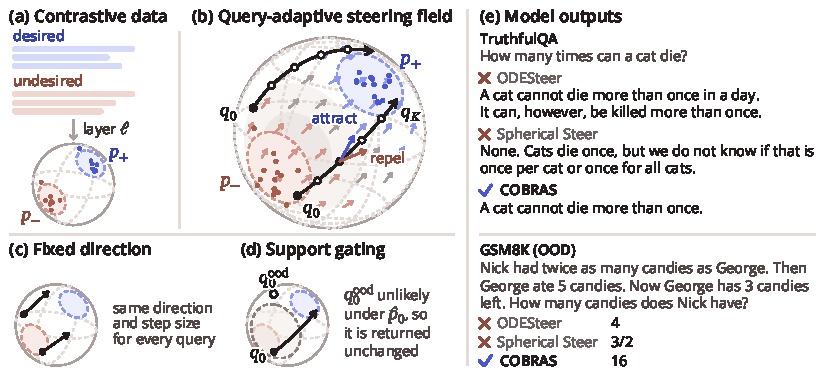
\includegraphics[width=0.8\linewidth]{figures/cobras_overview.pdf}
    \caption{Overview of \Cobras. \textbf{(a)} Contrastive activations at layer $\ell$ are projected onto
    $\Sph$. \textbf{(b)} Entropic optimal transport fits a coupling between the two populations. At each
    steering step, the coupling and the current activation determine weights for attraction toward desired
    samples and repulsion from undesired samples. \textbf{(c--d)} Whereas a fixed intervention treats every
    activation alike, \Cobras adjusts its direction and strength to the input; its support gate can leave
    unfamiliar prompts unchanged. \textbf{(e)} Example generations for TruthfulQA and an out-of-distribution
    GSM8K question, compared with ODESteer. The figure's iterates $q_k$ and support score $\hat p_0$
    correspond to $\boldsymbol{x}_k$ and $\hat p_{b_g}$ in the text.}
    \label{fig:overview}
\end{figure}

\subsection{From a population transport problem to a steering field}
\label{subsec:sb}

A direction that increases the likelihood of the desired behavior need not specify how to transform the
whole undesired population into the desired one. We begin with this population-level problem. A path measure
$P$ assigns probabilities to trajectories $(\boldsymbol{x}_t)_{t\in[0,1]}$ on $\Sph$; its marginal $P_t$
is the distribution of activations at time $t$. Taking Brownian motion on $\Sph$ as the reference $Q$, the
Schr\"{o}dinger bridge solves

\begin{equation}
P^{\star} = \operatorname*{arg\,min}_{P}\;\KL(P \,\Vert\, Q)
\qquad\text{s.t.}\qquad
P_{0} = \pminus, \quad P_{1} = \pplus ,
\label{eq:sb}
\end{equation}

Here $\KL$ is relative entropy between path measures, and $Q$ starts from the uniform distribution with
diffusivity $\sigma^2>0$. Thus the endpoint constraints specify the behavioral change, while the objective
selects the evolution that departs least from the reference motion. The time variable $t$ indexes this
transport between populations; it is separate from the token positions in a generated sequence.

The classical bridge solution is described by two positive functions, called Schr\"{o}dinger
potentials~\citep{leonard2013survey, chen2021likelihood, chen2023deep}. The potential
$\varphi(\boldsymbol{x},t)$ propagates information forward from the undesired population, and
$\psi(\boldsymbol{x},t)$ propagates information backward from the desired population. Both are functions
from $\Sph\times(0,1)$ to $(0,\infty)$, and $\nablaS$ differentiates their spatial argument with $t$
held fixed. We reserve these unhatted symbols for the continuous bridge; empirical kernel factors below
carry hats and explicit bandwidth subscripts. Their product gives the bridge's marginal density:

\begin{equation}
p_{t}(\boldsymbol{x})\;\propto\;\varphi(\boldsymbol{x},t)\,\psi(\boldsymbol{x},t),
\qquad
p_{0}(\boldsymbol{x})=\pminus(\boldsymbol{x}),\quad p_{1}(\boldsymbol{x})=\pplus(\boldsymbol{x}) .
\label{eq:product}
\end{equation}

Intuitively, $\varphi(\boldsymbol{x},t)$ describes how strongly the starting population reaches $\boldsymbol{x}$ at time
$t$, while $\psi(\boldsymbol{x},t)$ describes how strongly $\boldsymbol{x}$ connects to the target population in the
remaining time. The endpoint constraints determine the potentials, and the bridge adds the drift
$\sigma^2\nablaS\log\psi(\boldsymbol{x},t)$ to the reference diffusion.

To turn this stochastic evolution into a deterministic activation edit, we use its probability-flow ODE.
For the continuous bridge, this ODE has the same time marginals as the stochastic
process~\citep{song2020score}. Subtracting the diffusion contribution
$\tfrac{\sigma^2}{2}\nablaS\log p_t(\boldsymbol{x})$ from the bridge drift and using Eq.~\eqref{eq:product} gives
(Appendix~\ref{apx:static})

\begin{equation}
d\boldsymbol{x}_{t}
= \frac{\sigma^{2}}{2}\,\nablaS\log
  \frac{\psi(\boldsymbol{x}_{t},t)}{\varphi(\boldsymbol{x}_{t},t)}\,dt .
\label{eq:ldr}
\end{equation}

The two potentials therefore serve complementary purposes: their log-ratio supplies a direction toward
the desired population and away from the undesired one, while their product describes where the bridge
places probability mass. These identities motivate the direction and support score used below. Applying
them to finite samples and individual token activations requires the kernel construction and conditioning
choices in the next subsection.

\subsection{Computing the direction from contrastive samples}
\label{subsec:estimation}

\paragraph{Fit a transport plan offline.}
We first construct a coupling between the projected samples in $\mathcal{D}^{-}$ and $\mathcal{D}^{+}$.
The continuous bridge admits a static formulation over its endpoint coupling
(Appendix~\ref{apx:static}); we discretize that formulation using the empirical populations. To measure
proximity on $\Sph$, we use the geodesic kernel

\begin{equation}
K_{b}(\boldsymbol{x},\boldsymbol{y})
= \exp\!\left(-\frac{d_{\Sph}(\boldsymbol{x},\boldsymbol{y})^{2}}{2b}\right), \qquad b>0,
\label{eq:kernel}
\end{equation}

where $b$ has units of squared distance. Its form is motivated by the leading short-time behavior of the
Brownian transition density~\citep{de2022riemannian, chen2023logarithmic}. At our operating scale we use
$K_b$ as a chosen affinity kernel, rather than identifying it with the exact spherical heat kernel
(Remark~\ref{rem:prop1-tightness}).

Entropic optimal transport with this kernel yields the factorized plan

\begin{equation}
\pi^{\star}_{ji}=a^{-}_{j}\,a^{+}_{i}\,e^{-c_{ji}},
\qquad
c_{ji} = \frac{d_{\Sph}(\boldsymbol{h}^{-}_{j},\,\boldsymbol{h}^{+}_{i})^{2}}{2\varepsilon},
\label{eq:plan}
\end{equation}

The entry $\pi^\star_{ji}$ is the mass assigned from undesired sample $j$ to desired sample $i$.
The cost favors nearby pairs, and $\varepsilon=\sigma^2$ sets the entropic scale. The \emph{scalings}
$a^{-}_{j}>0$ and $a^{+}_{i}>0$ are scalar weights attached to samples.
We collect them in $\boldsymbol{a}^{-}=(a^{-}_{j})_{j=1}^{N_-}$ and
$\boldsymbol{a}^{+}=(a^{+}_{i})_{i=1}^{N_+}$. For the fixed data and entropic scale, these weights enforce
the empirical marginals: each row must sum to $1/N_-$ and each column to $1/N_+$.
We obtain them with alternating Sinkhorn updates~\citep{cuturi2013sinkhorn},

\begin{equation}
\log a^{-}_{j} = -\log N_{-} - \operatorname{logsumexp}_{i}\left[\log a^{+}_{i} - c_{ji}\right],
\qquad
\log a^{+}_{i} = -\log N_{+} - \operatorname{logsumexp}_{j}\left[\log a^{-}_{j} - c_{ji}\right].
\label{eq:sinkhorn}
\end{equation}

The resulting plan minimizes expected cost plus negative entropy over couplings with these marginals.
Its costs and scalings are computed once for a given contrastive dataset, model, and steering layer.

\paragraph{Evaluate the potentials at an activation.}
To obtain a steering direction at a token's current activation $\boldsymbol{x}\in\Sph$, we first extend
the fitted sample weights to empirical potential functions. Each sample contributes its kernel affinity
to $\boldsymbol{x}$, weighted by its Sinkhorn scaling, so the desired and undesired populations define

\begin{equation}
\widehat{\psi}_{b}(\boldsymbol{x}) = \sum\nolimits_{i=1}^{N_{+}}a^{+}_{i}\,K_{b}(\boldsymbol{x},\boldsymbol{h}^{+}_{i}),
\qquad
\widehat{\varphi}_{b}(\boldsymbol{x}) = \sum\nolimits_{j=1}^{N_{-}}a^{-}_{j}\,K_{b}(\boldsymbol{x},\boldsymbol{h}^{-}_{j}),
\label{eq:frozen-factors}
\end{equation}

where the evaluation bandwidth $b>0$ controls how broadly each population contributes around
$\boldsymbol{x}$, while $\varepsilon$ determines the transport plan fitted offline. In the continuous
bridge, the two potentials use bandwidths associated with elapsed and remaining transport time.
Because a decoded token has no prescribed bridge time, we use a common, fixed $b$ to construct a
stationary steering field; the continuous bridge's endpoint-matching guarantee applies to its
time-dependent evolution.

Following the log-ratio direction in Eq.~\eqref{eq:ldr}, we take the difference of the two empirical
potentials' log-gradients. For the geodesic kernel, the identity
$\nablaS d_{\Sph}(\boldsymbol{x},\boldsymbol{h})^2=-2\log_{\boldsymbol{x}}(\boldsymbol{h})$ expresses
each log-gradient as a weighted average of tangent vectors toward the samples. For the desired population,
this gives

\begin{equation}
\nablaS\log\widehat{\psi}_{b}(\boldsymbol{x})
= \frac{1}{b}\sum_{i=1}^{N_{+}} w^{+}_{i}(\boldsymbol{x})\,\log_{\boldsymbol{x}}(\boldsymbol{h}^{+}_{i}),
\qquad
w^{+}_{i}(\boldsymbol{x})
= \mathrm{softmax}_{i}\!\left[\log a^{+}_{i}
   - \frac{d_{\Sph}(\boldsymbol{x},\boldsymbol{h}^{+}_{i})^{2}}{2b}\right],
\label{eq:grad-psi}
\end{equation}

with the corresponding expression for $\nablaS\log\widehat{\varphi}_{b}(\boldsymbol{x})$ obtained by
summing over $\mathcal{D}^{-}$ (Appendix~\ref{app:grad-psi}); both identities hold away from the samples'
antipodes. The normalized weight $w_i^{+}(\boldsymbol{x})$ combines the desired sample's proximity to
$\boldsymbol{x}$ with its fitted scaling $a_i^{+}$. Subtracting the undesired log-gradient therefore
combines attraction toward desired samples with repulsion from undesired samples, providing the
weighted log-map construction that we refine below.

\paragraph{Condition the weights on the current activation.}
The weights in Eq.~\eqref{eq:grad-psi} use the transport plan through a single fitted scaling for each
sample. To make the direction depend on which samples the plan connects near $\boldsymbol{x}$,
\Cobras replaces these scalings with conditional multipliers. For a desired sample $i$, we aggregate
its connections to undesired samples, weighting each connection by the undesired sample's proximity
to $\boldsymbol{x}$. Applying the same construction from desired samples to an undesired sample $j$
gives the two positive multiplier functions

\begin{align}
\log m^{+}_{i,b}(\boldsymbol{x})
&= \operatorname{logsumexp}_{j}\!\left[
   \log a^{-}_{j}
   - \frac{d_{\Sph}(\boldsymbol{x},\boldsymbol{h}^{-}_{j})^{2}}{2b}
   - c_{ji}\right],
\label{eq:ext-psi}\\[2pt]
\log m^{-}_{j,b}(\boldsymbol{x})
&= \operatorname{logsumexp}_{i}\!\left[
   \log a^{+}_{i}
   - \frac{d_{\Sph}(\boldsymbol{x},\boldsymbol{h}^{+}_{i})^{2}}{2b}
   - c_{ji}\right].
\label{eq:ext-phi}
\end{align}

In the first expression, the kernel centered at $\boldsymbol{x}$ emphasizes nearby undesired samples,
and the pairwise cost $c_{ji}$ determines how strongly each sample in that neighborhood contributes to
desired sample $i$. The relation
$a^{+}_{i}m^{+}_{i,b}(\boldsymbol{x})=\sum_j\pi^\star_{ji}K_b(\boldsymbol{x},\boldsymbol{h}^{-}_j)$
identifies $m^{+}_{i,b}(\boldsymbol{x})$ as the kernel-weighted transport mass arriving at desired sample $i$,
divided by its scaling $a_i^{+}$. We then combine the multiplier with the desired sample's own
proximity to $\boldsymbol{x}$ and normalize across desired samples. The resulting weights and
steering field are

\begin{align}
\bar{w}^{+}_{i}(\boldsymbol{x})
&= \mathrm{softmax}_{i}\!\left[
  \log m^{+}_{i,b}(\boldsymbol{x})
  - \frac{d_{\Sph}(\boldsymbol{x},\boldsymbol{h}^{+}_{i})^{2}}{2b}\right],
\label{eq:weights-pos}\\[2pt]
\boldsymbol{v}(\boldsymbol{x})
&= \sum\nolimits_{i=1}^{N_{+}} \bar{w}^{+}_{i}(\boldsymbol{x})\,\log_{\boldsymbol{x}}(\boldsymbol{h}^{+}_{i})
- \sum\nolimits_{j=1}^{N_{-}} \bar{w}^{-}_{j}(\boldsymbol{x})\,\log_{\boldsymbol{x}}(\boldsymbol{h}^{-}_{j}),
\label{eq:cobras-field}
\end{align}

where $\bar w_j^{-}(\boldsymbol{x})$ is obtained by replacing $m^{+}_{i,b}(\boldsymbol{x})$ and
$\boldsymbol{h}_i^{+}$ with $m^{-}_{j,b}(\boldsymbol{x})$ and $\boldsymbol{h}_j^{-}$ and normalizing
over undesired samples. Thus attraction and repulsion each depend on proximity within one population
and transport connections to the other population near $\boldsymbol{x}$. Since the integrator
normalizes $\boldsymbol{v}(\boldsymbol{x})$ before stepping, we omit the common prefactors $1/b$ and
$\sigma^2/2$.

At each steering iterate, we recompute the conditional multipliers at the updated activation and
use them as fixed coefficients in the weighted log-map construction. This defines the field in
Eq.~\eqref{eq:cobras-field}; differentiating through the multipliers would introduce additional terms
derived in Appendix~\ref{apx:omitted-term}. The common bandwidth $b$ makes this construction and its
density-ratio limit explicit, while the implementation selects bandwidths separately for each activation
and population. Appendix~\ref{app:grad-psi} describes this adaptive choice and compares it with the
fixed-bandwidth version.

\subsection{Controlling when and how much to steer}
\label{subsec:strength}

We follow the normalized direction $\boldsymbol{v}/\lVert\boldsymbol{v}\rVert$, so its magnitude cannot
reduce the intervention on a token that already exhibits the desired behavior or on an unfamiliar prompt.
We handle these cases with two factors in $[0,1]$: a per-token side factor $s$ and a per-prompt support gate
$g$. Their product scales the user-selected steering strength $T$.

\paragraph{Side factor: reduce steering on the desired side.}
We estimate which side of the behavioral boundary the current token occupies using a simple auxiliary
class model. Let $\bar{\boldsymbol{h}}^{\pm}$ be the means of the projected contrastive samples. Model
the classes by von Mises--Fisher distributions with opposite mean directions $\pm\boldsymbol{\mu}$,
equal prior probabilities, and shared concentration $\kappa$. The class axis and posterior probability of
the undesired class are

\begin{align}
\boldsymbol{\mu}
&= \frac{\bar{\boldsymbol{h}}^{+}-\bar{\boldsymbol{h}}^{-}}
       {\lVert\bar{\boldsymbol{h}}^{+}-\bar{\boldsymbol{h}}^{-}\rVert},
\label{eq:mu}\\[2pt]
s(\boldsymbol{x}) &= \bigl(1+e^{\,2\kappa\langle\boldsymbol{x}/R,\,\boldsymbol{\mu}\rangle}\bigr)^{-1}.
\label{eq:side}
\end{align}

The shared normalizing constants cancel, giving log-odds
$2\kappa\langle\boldsymbol{x}/R,\boldsymbol{\mu}\rangle$ in favor of the desired class
(Appendix~\ref{apx:ldr-formalize}). Consequently, $s$ is larger on the undesired side, equals $1/2$ at the
boundary, and decreases smoothly on the desired side. It attenuates steering rather than imposing a hard
stop at the boundary. We evaluate $s$ on each token's incoming activation and hold it fixed during that
token's integration steps.

\paragraph{Support gate: reduce steering on unfamiliar prompts.}
A class posterior alone cannot determine whether the fitted intervention is appropriate for a prompt.
For example, a truthfulness intervention may alter a math problem whose activations lie far from the
contrastive samples. A ratio can remain large even when both of its factors are small. Their product
retains this information, motivating a support score based on Eq.~\eqref{eq:product}. Using the fixed
Sinkhorn scalings and a gate bandwidth $b_g$, we define

\begin{equation}
\begin{aligned}
u(\boldsymbol{x}) &= -\log\hat p_{b_{g}}(\boldsymbol{x}), \\
\log\hat p_{b_{g}}(\boldsymbol{x})
&= \operatorname{logsumexp}_{j}\!\left[\log a^{-}_{j}
  -\frac{d_{\Sph}(\boldsymbol{x},\boldsymbol{h}^{-}_{j})^{2}}{2b_{g}}\right] \\
&\quad + \operatorname{logsumexp}_{i}\!\left[\log a^{+}_{i}
  -\frac{d_{\Sph}(\boldsymbol{x},\boldsymbol{h}^{+}_{i})^{2}}{2b_{g}}\right],
\end{aligned}
\label{eq:support-score}
\end{equation}

Here $\hat p_{b_g}(\boldsymbol{x})=\widehat{\varphi}_{b_g}(\boldsymbol{x})\widehat{\psi}_{b_g}(\boldsymbol{x})$ is an unnormalized support score built from the kernel
factors; large $u$ indicates low support. At this chosen bandwidth it serves as a proxy for the bridge
marginal, rather than an exact time marginal of the continuous bridge. As $b_g\to0$, $2b_gu(\boldsymbol{x})$
approaches the sum of squared distances to the nearest sample in each population
(Lemma~\ref{lem:gate-nn}). The score thus connects the potential product to a local measure of proximity
to the contrastive data.

To interpret this score on the inputs encountered at inference, we calibrate it on in-distribution
\emph{prompt} activations $\mathcal{D}_{\mathrm{ref}}$, held out from evaluation. Each reference activation
is taken at layer $\ell$ and the last prompt position, and projected onto $\Sph$ before scoring. We rank a
query's score against these reference scores and convert its rank to a gate:

\begin{equation}
r(\boldsymbol{x})
= \frac{\bigl|\{\boldsymbol{z}\in\mathcal{D}_{\mathrm{ref}} : u(\boldsymbol{z}) < u(\boldsymbol{x})\}\bigr|}
       {|\mathcal{D}_{\mathrm{ref}}|},
\qquad
g(\boldsymbol{x}) = \mathrm{clamp}\!\left(\frac{1-r(\boldsymbol{x})}{1-p},\,0,\,1\right),
\label{eq:gate}
\end{equation}

The coverage parameter $p\in(0,1)$ sets the rank below which the gate is one. Above that rank the gate
decreases linearly, reaching zero when the query score exceeds all reference scores. We compute
$g_q$ once on the last prompt token and hold it fixed throughout generation, so a prompt with $g_q=0$
receives no steering. The ungated configuration sets $g_q=1$ directly.

Calibration on prompts matches the layer and token position where the gate is used, rather than assuming
that contrastive question--answer activations have the same score distribution. It requires no OOD data.
Under the continuous in-distribution percentile model, a fraction $p$ of prompts receives full strength
and $\mathbb{E}[g]=(1+p)/2$; a finite reference set introduces rank discretization
(Appendix~\ref{apx:ood-gate}). These are calibration properties, while separation of unfamiliar prompts
depends on their scores. The appendix reports the measured in-distribution coverage and OOD separation.

\subsection{Applying the intervention during generation}
\label{subsec:procedure}

The direction and strength controls now define the activation edit. For the incoming activation
$\hquery$, set $\boldsymbol{x}_0=R\hquery/\lVert\hquery\rVert$, evaluate $s(\boldsymbol{x}_0)$, and use
the prompt's cached gate $g_q$. With $K$ geodesic Euler steps, the update is

\begin{equation}
\Delta = \frac{\pi}{2}\,T\,s(\boldsymbol{x}_{0})\,g_{q}\,\frac{R}{K},
\qquad
\boldsymbol{x}_{k+1}
= \exp_{\boldsymbol{x}_{k}}\!\left(\Delta\,
  \frac{\boldsymbol{v}(\boldsymbol{x}_{k})}{\lVert\boldsymbol{v}(\boldsymbol{x}_{k})\rVert}\right),
\label{eq:step}
\end{equation}

Each nonzero step traverses an arc of length $\Delta$. At full strength ($s=g_q=1$), the total path length
is $\tfrac{\pi}{2}TR$, so $T$ expresses the steering budget in units of a quarter great circle.
We recompute the conditional multipliers and direction at every iterate, while keeping $s$ and $g_q$
fixed during these $K$ steps. After integration, the activation returned to the model is
$\lVert\hquery\rVert\boldsymbol{x}_K/R$, which restores its original norm. If the step length or field
is zero, the corresponding update is zero.

\paragraph{Offline preparation and online cost.}
For each contrastive dataset, model, and layer, preparation projects the samples onto $\Sph$, sets the
transport scale from their spacing, fits the Sinkhorn scalings, and computes the class axis and reference
support scores. During generation, the intervention runs on the last-token activation at each decoding
step, starting with the last prompt token. No model weights change. For the dense construction shown
here, each field evaluation uses $O(N_-N_+)$ work to form the conditional multipliers and
$O(d(N_-+N_+))$ work for distances and weighted tangent vectors; the transport cost matrix is stored
offline. Each steered token requires $K$ such evaluations.
Algorithm~\ref{alg:cobras} gives the pseudocode, and
Appendix~\ref{appendix:implementation_details} lists the experimental settings.

The bridge supplies the log-ratio form of the direction and the product form of the support score.
\Cobras turns those identities into a practical intervention through the geodesic kernel, conditional
weights, normalized steps, and strength controls. Its endpoint transport objective motivates these
operations; exact population transport is not a guarantee of the resulting token-level procedure.

\subsection{Connection to density-ratio steering}
\label{subsec:reduction}

We now relate the construction to a familiar steering objective. Several methods can be expressed as
following a log-density-ratio gradient~\citep{rimsky2024steering, zhaoodesteer, li2023inference},

\begin{equation}
  \boldsymbol{v}(\boldsymbol{x}) \;\propto\; \nabla \log \frac{\pplus(\boldsymbol{x})}{\pminus(\boldsymbol{x})},
  \label{eq:ldr-ideal}
\end{equation}

which combines attraction toward regions favored by $\pplus$ with repulsion from regions favored by
$\pminus$. For isotropic Gaussians $\mathcal{N}(\boldsymbol{\mu}_{\pm},\boldsymbol{I}_d)$, this gradient
is the constant vector $\boldsymbol{\mu}_+-\boldsymbol{\mu}_-$ used by Contrastive Activation Addition
(CAA)~\citep{rimsky2024steering}. Appendix~\ref{apx:ldr-formalize} and
Table~\ref{tab:steering_framework} describe the corresponding parameterizations for other methods.

The bridge provides a population transport objective from which a log-ratio field follows. For the
sample-based construction, the ordinary kernel density-ratio field is recovered when transport costs
become negligible. Define

\begin{equation}
\hat p^{\pm}_{b}(\boldsymbol{x})
= \frac{1}{N_{\pm}}\sum\nolimits_{k=1}^{N_{\pm}} K_{b}(\boldsymbol{x},\boldsymbol{h}^{\pm}_{k}),
\qquad
\boldsymbol{v}^{\mathrm{kde}}_{b}(\boldsymbol{x})
= b\,\nablaS\log\frac{\hat p^{+}_{b}(\boldsymbol{x})}{\hat p^{-}_{b}(\boldsymbol{x})}
\label{eq:ldr-kde}
\end{equation}

where the kernel's common normalizing constant cancels in the ratio. By Eq.~\eqref{eq:grad-psi}, this
field uses uniform multipliers within each population. As $\varepsilon$ grows, the costs $c_{ji}$ tend
to zero, the reference weights $K_{\varepsilon}(\boldsymbol{h}^{-}_{j},\boldsymbol{h}^{+}_{i})$ become uniform, and the optimal coupling approaches the
independent plan $\pi^\star_{ji}=1/(N_-N_+)$. The following proposition quantifies how the conditional
field approaches the kernel density-ratio field in this regime.

\begin{proposition}[Reduction to the kernel density-ratio drift]
\label{prop:ldr-limit}
Fix $\mathcal{D}^{\pm}\subset\Sph$, an entropic scale $\varepsilon>0$ and an evaluation bandwidth $b>0$, put
$c_{\max}=\max_{j,i}c_{ji}$, and let $(\boldsymbol{a}^{-},\boldsymbol{a}^{+})$ be an iterate obtained after a complete
Sinkhorn sweep of Eq.~\eqref{eq:sinkhorn}, or its fixed point. Then at every $\boldsymbol{x}\in\Sph$ not antipodal to
a sample, the field of Eq.~\eqref{eq:cobras-field} satisfies
\begin{equation}
\bigl\lVert\,\boldsymbol{v}(\boldsymbol{x})-\boldsymbol{v}^{\mathrm{kde}}_{b}(\boldsymbol{x})\,\bigr\rVert
\;\le\; 2\pi R\,\bigl(e^{c_{\max}}-1\bigr).
\label{eq:prop1-bound}
\end{equation}
Since $c_{\max}\le\pi^{2}R^{2}/(2\varepsilon)$, holding $\mathcal{D}^{\pm}$ and $b$ fixed and letting
$\varepsilon\to\infty$ drives the right-hand side to zero, so $\boldsymbol{v}$ converges to
$\boldsymbol{v}^{\mathrm{kde}}_{b}$ uniformly over points that are not antipodal to a sample.
\end{proposition}

The limit holds at a fixed evaluation bandwidth $b$: it removes the information carried by the coupling
while retaining a nondegenerate kernel density-ratio field. At finite $\varepsilon$, the transport
weights modify that field using relationships between the two populations. The bound gives an asymptotic
$O(1/\varepsilon)$ rate; it is not tight at our operating scale
(Remark~\ref{rem:prop1-tightness}). The proof is in Appendix~\ref{apx:proof-ldr-limit}.

A separate statistical question is whether the kernel estimates recover the population objective in
Eq.~\eqref{eq:ldr-ideal}. Under the smoothness and sampling conditions of Remark~\ref{rem:consistency},
shrinking $b$ with sample size gives consistency of the unscaled log-density-ratio gradient wherever both
population densities are bounded away from zero. That sampling limit differs from the fixed-$b$ transport
limit above and does not provide a combined guarantee for the deployed steering procedure.

\vspace{-1mm}
\section{Experiments}
\label{sec:exp}
\vspace{-1mm}

We evaluate whether \Cobras improves the target behavior while preserving other capabilities, and how its components affect performance and computational cost. We address three research questions. \textbf{(RQ1):} How does \Cobras compare to other steering methods on in-distribution tasks? \textbf{(RQ2):} How well does \Cobras preserve model capabilities under distribution shift? \textbf{(RQ3):} How do the design choices affect performance and computational cost?

\noindent\textbf{Datasets.}~We conduct our evaluations on three prevalent steering datasets: TruthfulQA~\cite{lin2021truthfulqa} (TQA) for Truthfulness, UltraFeedback~\cite{cui2023ultrafeedback} (UF) for Helpfulness and RealToxicityPrompts~\cite{gehman2020realtoxicityprompts} for Detoxification. With steering fitted on TruthfulQA, we evaluate out-of-distribution performance on Natural Questions~\cite{kwiatkowski2019natural} (NQ) and TriviaQA~\cite{joshi2017triviaqa} for within-task shifts, and MMLU~\cite{hendrycks2020measuring} and GSM8K~\cite{cobbe2021gsm8k} for cross-task shifts.

\noindent\textbf{Baselines and models.}~Following ODESteer~\cite{zhaoodesteer}, we compare \Cobras against the following baselines: Representation Engineering~\citep{zou2023representation} (RepE), Inference-Time Intervention~\citep{li2023inference} (ITI), Contrastive Activation Addition~\citep{rimsky2024steering} (CAA), Minimally Modified Counterfactuals~\citep{singh2024representation} (MiMiC), Linear Activation Transport~\citep{rodriguez2025controlling} (Linear-AcT),  SphericalSteering~\cite{you2026spherical} and ODESteer~\cite{zhaoodesteer}. We test the steering methods on four open-source models: Falcon-7B~\citep{almazrouei2023falcon}, Mistral-7B~\citep{jiang2023mistral7b}, LLaMA3.1-8B~\citep{meta2024llama3.1} and Qwen2.5-7B~\cite{qwen2.5}.

\noindent\textbf{Metrics.}~Following ODESteer~\cite{zhaoodesteer}, we use Truthfulness $\times$ Informativeness (\%) as the primary metric for TQA and report Truthfulness (\%) and Informativeness (\%). For UF, we use win rate over the unsteered model (primary), mean reward, and 90th percentile reward. For detoxification, we use toxicity from the Perspective API~\cite{perspective_api} (primary), perplexity, and Dist-2. For GSM8K and MMLU, we use accuracy. See Appendix~\ref{appendix:metrics} for details.

\begin{table*}[t]
\centering
\caption{Performance of steering methods on Helpfulness (UltraFeedback), Truthfulness (TruthfulQA), and Detoxification (RealToxicityPrompts) for four LLMs. Results are means $\pm$ standard deviations over three runs with different seeds. Primary metrics are highlighted in light purple.
}
\large
\renewcommand{\arraystretch}{1.2}
\resizebox{0.96\linewidth}{!}{%
\begin{tabular}{cc|
c c >{\columncolor{lightpurple!25}}c|
c c >{\columncolor{lightpurple!25}}c|
c c >{\columncolor{lightpurple!25}}c}

\toprule[1.5pt]
\multirow{2}{*}{\textbf{Method}} & \multirow{2}{*}{\textbf{Model}} &
\multicolumn{3}{c|}{\textbf{Helpfulness} \textsubscript{\scriptsize\textbf{(UltraFeedback)}}} &
\multicolumn{3}{c|}{\textbf{Truthfulness} \textsubscript{\scriptsize\textbf{(TruthfulQA)}}} &
\multicolumn{3}{c}{\textbf{Detoxification} \textsubscript{\scriptsize{(RealToxicityPrompts)}}} \\
\cmidrule(lr){3-5}\cmidrule(lr){6-8}\cmidrule(lr){9-11}
&  & \textbf{RM$_{\text{mean}}$}\,$\boldsymbol{\uparrow}$ & \textbf{RM$_{\text{P90}}$}\,$\boldsymbol{\uparrow}$ & \textbf{Win (\%)}\,$\boldsymbol{\uparrow}$
& \textbf{True (\%)}\,$\boldsymbol{\uparrow}$ & \textbf{Info (\%)}\,$\boldsymbol{\uparrow}$ & \textbf{T$\times$I (\%)}\,$\boldsymbol{\uparrow}$
 & \textbf{PPL}\,$\boldsymbol{\downarrow}$ & \textbf{Dist-2}\,$\boldsymbol{\uparrow}$ & \textbf{ Toxic }\,$\boldsymbol{\downarrow}$ \\
\midrule


Original & \multirow{9}{*}{\rotatebox[origin=c]{90}{Falcon-7B}} & -12.642 {\tiny $\pm$ 0.162} & -2.705 {\tiny $\pm$ 0.171} & 50.0 {\tiny $\pm$ 0.000} & 32.1 {\tiny $\pm$ 0.951} & 96.5 {\tiny $\pm$ 0.283} & 29.1 {\tiny $\pm$ 0.919} & 15.358 {\tiny $\pm$ 0.449} & 0.946 {\tiny $\pm$ 0.003} & 0.255 {\tiny $\pm$ 0.004} \\\midrule



RepE &  & -12.711 {\tiny $\pm$ 0.270} & -2.680 {\tiny $\pm$ 0.099} & 50.2 {\tiny $\pm$ 0.981} & 31.7 {\tiny $\pm$ 0.982} & 96.6 {\tiny $\pm$ 0.308} & 28.7 {\tiny $\pm$ 1.069} & 15.371 {\tiny $\pm$ 0.178} & 0.941 {\tiny $\pm$ 0.003} & 0.232 {\tiny $\pm$ 0.010} \\

ITI &  & -12.789 {\tiny $\pm$ 0.221} & -2.866 {\tiny $\pm$ 0.134} & 49.0 {\tiny $\pm$ 1.358} & 36.8 {\tiny $\pm$ 0.738} & 95.5 {\tiny $\pm$ 0.393} & 32.8 {\tiny $\pm$ 0.616} & 15.707 {\tiny $\pm$ 0.346} & 0.941 {\tiny $\pm$ 0.005} & 0.239 {\tiny $\pm$ 0.004} \\

CAA &  & -12.540 {\tiny $\pm$ 0.226} & -2.260 {\tiny $\pm$ 0.410} & 49.9 {\tiny $\pm$ 2.346} & 42.0 {\tiny $\pm$ 1.905} & 95.4 {\tiny $\pm$ 0.494} & 37.9 {\tiny $\pm$ 1.495} & 75.550 {\tiny $\pm$ 9.063} & 0.852 {\tiny $\pm$ 0.002} & \textbf{0.076} {\tiny $\pm$ 0.007} \\

MiMiC &  & -12.751 {\tiny $\pm$ 0.136} & -2.678 {\tiny $\pm$ 0.213} & 50.7 {\tiny $\pm$ 1.350} & 43.3 {\tiny $\pm$ 0.374} & 88.3 {\tiny $\pm$ 0.927} & 32.9 {\tiny $\pm$ 0.764} & 15.026 {\tiny $\pm$ 0.258} & 0.941 {\tiny $\pm$ 0.004} & 0.240 {\tiny $\pm$ 0.009} \\

Linear-AcT &  & -12.412 {\tiny $\pm$ 0.205} & -2.534 {\tiny $\pm$ 0.309} & 50.8 {\tiny $\pm$ 1.300} & 44.3 {\tiny $\pm$ 0.534} & 95.0 {\tiny $\pm$ 0.212} & 40.0 {\tiny $\pm$ 0.561} & 16.113 {\tiny $\pm$ 0.206} & 0.947 {\tiny $\pm$ 0.002} & 0.240 {\tiny $\pm$ 0.003} \\


ODESteer &  & -12.446 {\tiny $\pm$ 0.050} & -2.806 {\tiny $\pm$ 0.207} & 49.7 {\tiny $\pm$ 1.210} & 35.4 {\tiny $\pm$ 0.534} & 96.2 {\tiny $\pm$ 0.441} & 32.1 {\tiny $\pm$ 0.674} & 15.709 {\tiny $\pm$ 0.405} & 0.940 {\tiny $\pm$ 0.002} & 0.188 {\tiny $\pm$ 0.006} \\

SphericalSteer &  & -12.495 {\tiny $\pm$ 0.120} & -3.108 {\tiny $\pm$ 0.244} & 49.5 {\tiny $\pm$ 2.255} & 62.9 {\tiny $\pm$ 1.469} & 71.6 {\tiny $\pm$ 1.534} & 37.7 {\tiny $\pm$ 1.354} & 21.542 {\tiny $\pm$ 1.543} & 0.924 {\tiny $\pm$ 0.008} & 0.147 {\tiny $\pm$ 0.011} \\

\midrule
\rowcolor{cobrasblue}\textbf{COBRAS (Ours)} &  & -12.24 {\tiny $\pm$ 0.336} & -2.601 {\tiny $\pm$ 0.121} & \textbf{52.8} {\tiny $\pm$ 2.628} & 45.5 {\tiny $\pm$ 2.124} & 93.4 {\tiny $\pm$ 1.379} & \textbf{40.3} {\tiny $\pm$ 1.390} & 15.304 {\tiny $\pm$ 0.591} & 0.942 {\tiny $\pm$ 0.005} & 0.138 {\tiny $\pm$ 0.012} \\

\midrule
\midrule
Original & \multirow{9}{*}{\rotatebox[origin=c]{90}{Mistral-7B}} & -11.063 {\tiny $\pm$ 0.377} & -0.469 {\tiny $\pm$ 0.752} & 50.0 {\tiny $\pm$ 0.000} & 41.7 {\tiny $\pm$ 0.764} & 94.8 {\tiny $\pm$ 0.463} & 36.9 {\tiny $\pm$ 0.616} & 18.542 {\tiny $\pm$ 0.498} & 0.990 {\tiny $\pm$ 0.001} & 0.207 {\tiny $\pm$ 0.008} \\\midrule


RepE &  & -11.981 {\tiny $\pm$ 0.377} & -1.622 {\tiny $\pm$ 0.423} & 45.3 {\tiny $\pm$ 2.237} & 42.0 {\tiny $\pm$ 0.674} & 93.9 {\tiny $\pm$ 0.490} & 36.1 {\tiny $\pm$ 1.055} & 76.065 {\tiny $\pm$ 1.734} & 0.969 {\tiny $\pm$ 0.001} & 0.218 {\tiny $\pm$ 0.004} \\

ITI &  & -11.116 {\tiny $\pm$ 0.310} & -1.229 {\tiny $\pm$ 0.311} & 48.8 {\tiny $\pm$ 0.611} & 54.2 {\tiny $\pm$ 1.616} & 92.6 {\tiny $\pm$ 1.041} & 47.3 {\tiny $\pm$ 1.952} & 18.956 {\tiny $\pm$ 0.170} & 0.989 {\tiny $\pm$ 0.000} & 0.181 {\tiny $\pm$ 0.013} \\

CAA &  & -10.424 {\tiny $\pm$ 0.144} & -0.601 {\tiny $\pm$ 0.439} & 53.7 {\tiny $\pm$ 4.636} & 74.7 {\tiny $\pm$ 0.212} & 88.2 {\tiny $\pm$ 1.278} & 63.2 {\tiny $\pm$ 0.989} & 18.912 {\tiny $\pm$ 0.281} & 0.991 {\tiny $\pm$ 0.001} & 0.167 {\tiny $\pm$ 0.011} \\

MiMiC &  & -11.511 {\tiny $\pm$ 0.324} & -0.676 {\tiny $\pm$ 0.535} & 48.5 {\tiny $\pm$ 2.751} & 50.2 {\tiny $\pm$ 2.124} & 91.2 {\tiny $\pm$ 1.176} & 41.6 {\tiny $\pm$ 1.019} & 18.922 {\tiny $\pm$ 0.781} & 0.989 {\tiny $\pm$ 0.001} & 0.192 {\tiny $\pm$ 0.010} \\


Linear-AcT &  & -10.448 {\tiny $\pm$ 0.191} & -0.139 {\tiny $\pm$ 0.544} & 53.0 {\tiny $\pm$ 4.996} & 48.4 {\tiny $\pm$ 0.738} & 94.0 {\tiny $\pm$ 0.141} & 42.7 {\tiny $\pm$ 0.796} & 18.784 {\tiny $\pm$ 0.320} & 0.990 {\tiny $\pm$ 0.001} & 0.189 {\tiny $\pm$ 0.009} \\

ODESteer &  & -10.951 {\tiny $\pm$ 0.275} & -0.622 {\tiny $\pm$ 0.041} & 54.8 {\tiny $\pm$ 3.946} & 73.9 {\tiny $\pm$ 1.443} & 91.1 {\tiny $\pm$ 0.141} & 65.2 {\tiny $\pm$ 1.619} & 21.081 {\tiny $\pm$ 0.156} & 0.993 {\tiny $\pm$ 0.001} & 0.101 {\tiny $\pm$ 0.008} \\

SphericalSteer &  & -11.005 {\tiny $\pm$ 0.126} & -1.958 {\tiny $\pm$ 0.337} & 50.3 {\tiny $\pm$ 2.948} & 76.6 {\tiny $\pm$ 1.324} & 83.7 {\tiny $\pm$ 0.510} & 60.8 {\tiny $\pm$ 1.630} & 21.295 {\tiny $\pm$ 0.122} & 0.990 {\tiny $\pm$ 0.001} & 0.099 {\tiny $\pm$ 0.005} \\

\midrule
\rowcolor{cobrasblue}\textbf{COBRAS (Ours)} &  & -10.261 {\tiny $\pm$ 0.163} & -0.157 {\tiny $\pm$ 0.621} & \textbf{57.1} {\tiny $\pm$ 3.253} & 85.2 {\tiny $\pm$ 0.972} & 80.3 {\tiny $\pm$ 0.982} & \textbf{66.4} {\tiny $\pm$ 1.901} & 20.631 {\tiny $\pm$ 0.330} & 0.992 {\tiny $\pm$ 0.001} & \textbf{0.096} {\tiny $\pm$ 0.006} \\

\midrule
\midrule

Original & \multirow{9}{*}{\rotatebox[origin=c]{90}{LLaMA3.1-8B}} & -10.303 {\tiny $\pm$ 0.145} & -0.744 {\tiny $\pm$ 0.435} & 50.0 {\tiny $\pm$ 0.000} & 45.1 {\tiny $\pm$ 1.309} & 97.6 {\tiny $\pm$ 0.628} & 43.0 {\tiny $\pm$ 1.496} & 18.562 {\tiny $\pm$ 0.107} & 0.992 {\tiny $\pm$ 0.001} & 0.218 {\tiny $\pm$ 0.002} \\\midrule


RepE &  & -10.763 {\tiny $\pm$ 0.295} & -1.356 {\tiny $\pm$ 0.378} & 47.1 {\tiny $\pm$ 1.050} & 46.2 {\tiny $\pm$ 0.989} & 97.4 {\tiny $\pm$ 0.187} & 43.9 {\tiny $\pm$ 1.041} & 19.101 {\tiny $\pm$ 0.496} & 0.991 {\tiny $\pm$ 0.001} & 0.195 {\tiny $\pm$ 0.003} \\

ITI &  & -10.138 {\tiny $\pm$ 0.232} & -0.739 {\tiny $\pm$ 0.611} & 51.5 {\tiny $\pm$ 2.026} & 57.3 {\tiny $\pm$ 0.902} & 95.8 {\tiny $\pm$ 0.374} & 53.6 {\tiny $\pm$ 1.055} & 18.698 {\tiny $\pm$ 0.377} & 0.990 {\tiny $\pm$ 0.002} & 0.190 {\tiny $\pm$ 0.011} \\

CAA &  & -9.966 {\tiny $\pm$ 0.132} & -0.628 {\tiny $\pm$ 0.380} & 50.9 {\tiny $\pm$ 0.874} & 68.1 {\tiny $\pm$ 2.221} & 92.6 {\tiny $\pm$ 0.495} & 61.0 {\tiny $\pm$ 2.020} & 19.647 {\tiny $\pm$ 0.349} & 0.992 {\tiny $\pm$ 0.001} & 0.152 {\tiny $\pm$ 0.005} \\

MiMiC &  & -9.713 {\tiny $\pm$ 0.175} & -0.549 {\tiny $\pm$ 0.112} & 54.9 {\tiny $\pm$ 1.905} & 60.1 {\tiny $\pm$ 0.430} & 92.0 {\tiny $\pm$ 0.612} & 52.8 {\tiny $\pm$ 1.041} & 18.667 {\tiny $\pm$ 0.311} & 0.991 {\tiny $\pm$ 0.001} & 0.198 {\tiny $\pm$ 0.010} \\

Linear-AcT &  & -9.944 {\tiny $\pm$ 0.469} & -0.411 {\tiny $\pm$ 0.654} & 52.5 {\tiny $\pm$ 2.203} & 53.1 {\tiny $\pm$ 1.683} & 97.8 {\tiny $\pm$ 0.187} & 51.0 {\tiny $\pm$ 1.484} & 18.521 {\tiny $\pm$ 0.333} & 0.991 {\tiny $\pm$ 0.001} & 0.199 {\tiny $\pm$ 0.014} \\

ODESteer &  & -8.280 {\tiny $\pm$ 0.316} & 1.206 {\tiny $\pm$ 0.441} & 56.3 {\tiny $\pm$ 0.896} & 67.3 {\tiny $\pm$ 2.544} & 95.1 {\tiny $\pm$ 0.441} & 62.5 {\tiny $\pm$ 2.570} & 19.831 {\tiny $\pm$ 0.224} & 0.993 {\tiny $\pm$ 0.000} & 0.124 {\tiny $\pm$ 0.002} \\

SphericalSteer &  & -9.434 {\tiny $\pm$ 0.304} & -0.633 {\tiny $\pm$ 0.837} & 52.3 {\tiny $\pm$ 1.790} & 86.9 {\tiny $\pm$ 2.389} & 76.0 {\tiny $\pm$ 1.504} & 63.5 {\tiny $\pm$ 0.902} & 23.039 {\tiny $\pm$ 0.274} & 0.993 {\tiny $\pm$ 0.000} & 0.123 {\tiny $\pm$ 0.010} \\

\midrule

\rowcolor{cobrasblue}\textbf{COBRAS (Ours)} &  & -8.109 {\tiny $\pm$ 0.283} & 0.800 {\tiny $\pm$ 0.120} & \textbf{59.7} {\tiny $\pm$ 1.610} & 82.8 {\tiny $\pm$ 0.308} & 84.9 {\tiny $\pm$ 1.168} & \textbf{68.1} {\tiny $\pm$ 1.343} & 20.083 {\tiny $\pm$ 0.184} & 0.992 {\tiny $\pm$ 0.000} & \textbf{0.107} {\tiny $\pm$ 0.004} \\

\midrule
\midrule
Original & \multirow{9}{*}{\rotatebox[origin=c]{90}{Qwen2.5-7B}} & -6.006 {\tiny $\pm$ 0.208} & 4.384 {\tiny $\pm$ 0.378} & 50.0 {\tiny $\pm$ 0.000} & 78.3 {\tiny $\pm$ 0.578} & 86.4 {\tiny $\pm$ 0.764} & 64.8 {\tiny $\pm$ 0.707} & 22.166 {\tiny $\pm$ 0.369} & 0.989 {\tiny $\pm$ 0.001} & 0.194 {\tiny $\pm$ 0.001} \\\midrule


RepE &  & -6.011 {\tiny $\pm$ 0.202} & 4.504 {\tiny $\pm$ 0.271} & 48.8 {\tiny $\pm$ 0.300} & 78.7 {\tiny $\pm$ 0.927} & 86.5 {\tiny $\pm$ 1.111} & 65.3 {\tiny $\pm$ 1.429} & 22.620 {\tiny $\pm$ 0.681} & 0.990 {\tiny $\pm$ 0.000} & 0.196 {\tiny $\pm$ 0.002} \\

ITI &  & -6.034 {\tiny $\pm$ 0.373} & 4.349 {\tiny $\pm$ 0.408} & 49.9 {\tiny $\pm$ 1.054} & 78.7 {\tiny $\pm$ 0.956} & 86.0 {\tiny $\pm$ 0.857} & 65.0 {\tiny $\pm$ 0.374} & 22.617 {\tiny $\pm$ 0.895} & 0.990 {\tiny $\pm$ 0.001} & 0.184 {\tiny $\pm$ 0.005} \\

CAA &  & -5.957 {\tiny $\pm$ 0.072} & 4.659 {\tiny $\pm$ 0.312} & 50.0 {\tiny $\pm$ 1.587} & 81.2 {\tiny $\pm$ 1.111} & 86.4 {\tiny $\pm$ 1.534} & 67.7 {\tiny $\pm$ 2.093} & 28.218 {\tiny $\pm$ 1.014} & 0.982 {\tiny $\pm$ 0.002} & 0.119 {\tiny $\pm$ 0.005} \\

MiMiC &  & -5.980 {\tiny $\pm$ 0.133} & 4.753 {\tiny $\pm$ 0.312} & 50.2 {\tiny $\pm$ 1.023 } & 82.9 {\tiny $\pm$ 0.283} & 79.0 {\tiny $\pm$ 1.026} & 62.5 {\tiny $\pm$ 1.097} & 21.233 {\tiny $\pm$ 0.363} & 0.989 {\tiny $\pm$ 0.002} & 0.176 {\tiny $\pm$ 0.005} \\

Linear-AcT &  & -6.017 {\tiny $\pm$ 0.111} & 4.788 {\tiny $\pm$ 0.499} & 50.4 {\tiny $\pm$ 1.747} & 79.8 {\tiny $\pm$ 1.205} & 87.0 {\tiny $\pm$ 1.046} & 67.0 {\tiny $\pm$ 1.168} & 22.643 {\tiny $\pm$ 0.876} & 0.990 {\tiny $\pm$ 0.001} & 0.181 {\tiny $\pm$ 0.004} \\

ODESteer &  & -5.995 {\tiny $\pm$ 0.095} & 4.738 {\tiny $\pm$ 0.175} & 50.7 {\tiny $\pm$ 1.222} & 82.2 {\tiny $\pm$ 1.460} & 86.7 {\tiny $\pm$ 2.145} & 69.2 {\tiny $\pm$ 1.434} & 22.310 {\tiny $\pm$ 0.565} & 0.990 {\tiny $\pm$ 0.002} & 0.170 {\tiny $\pm$ 0.004} \\

SphericalSteer &  & -7.203 {\tiny $\pm$ 0.208} & 4.309 {\tiny $\pm$ 0.192} & 43.6 {\tiny $\pm$ 1.644} & 82.9 {\tiny $\pm$ 1.874} & 77.6 {\tiny $\pm$ 1.067} & 61.4 {\tiny $\pm$ 2.086} & 68.485 {\tiny $\pm$ 2.191} & 0.942 {\tiny $\pm$ 0.008} & 0.129 {\tiny $\pm$ 0.007} \\

\midrule
\rowcolor{cobrasblue}\textbf{COBRAS (Ours)} &  & -5.755 { \tiny$\pm$ 0.419} & 5.162 {\tiny $\pm$ 0.746} & \textbf{51.9} {\tiny $\pm$ 1.616} & 83.3 {\tiny $\pm$ 0.430} & 86.0 {\tiny $\pm$ 0.141} & \textbf{69.7} {\tiny $\pm$ 0.495} & 23.786 {\tiny $\pm$ 0.625} & 0.985 {\tiny $\pm$ 0.003} & \textbf{0.114} {\tiny $\pm$ 0.006} \\
\bottomrule[1.5pt]
\end{tabular}
}
\label{tab:main_results}
\end{table*}


%%%%%%%%%%%%%%%%%%%%%%%%%%%%%%%%%%%%%%%%%%%%%%%%%%%%%
\begin{figure}[t]
    \centering
    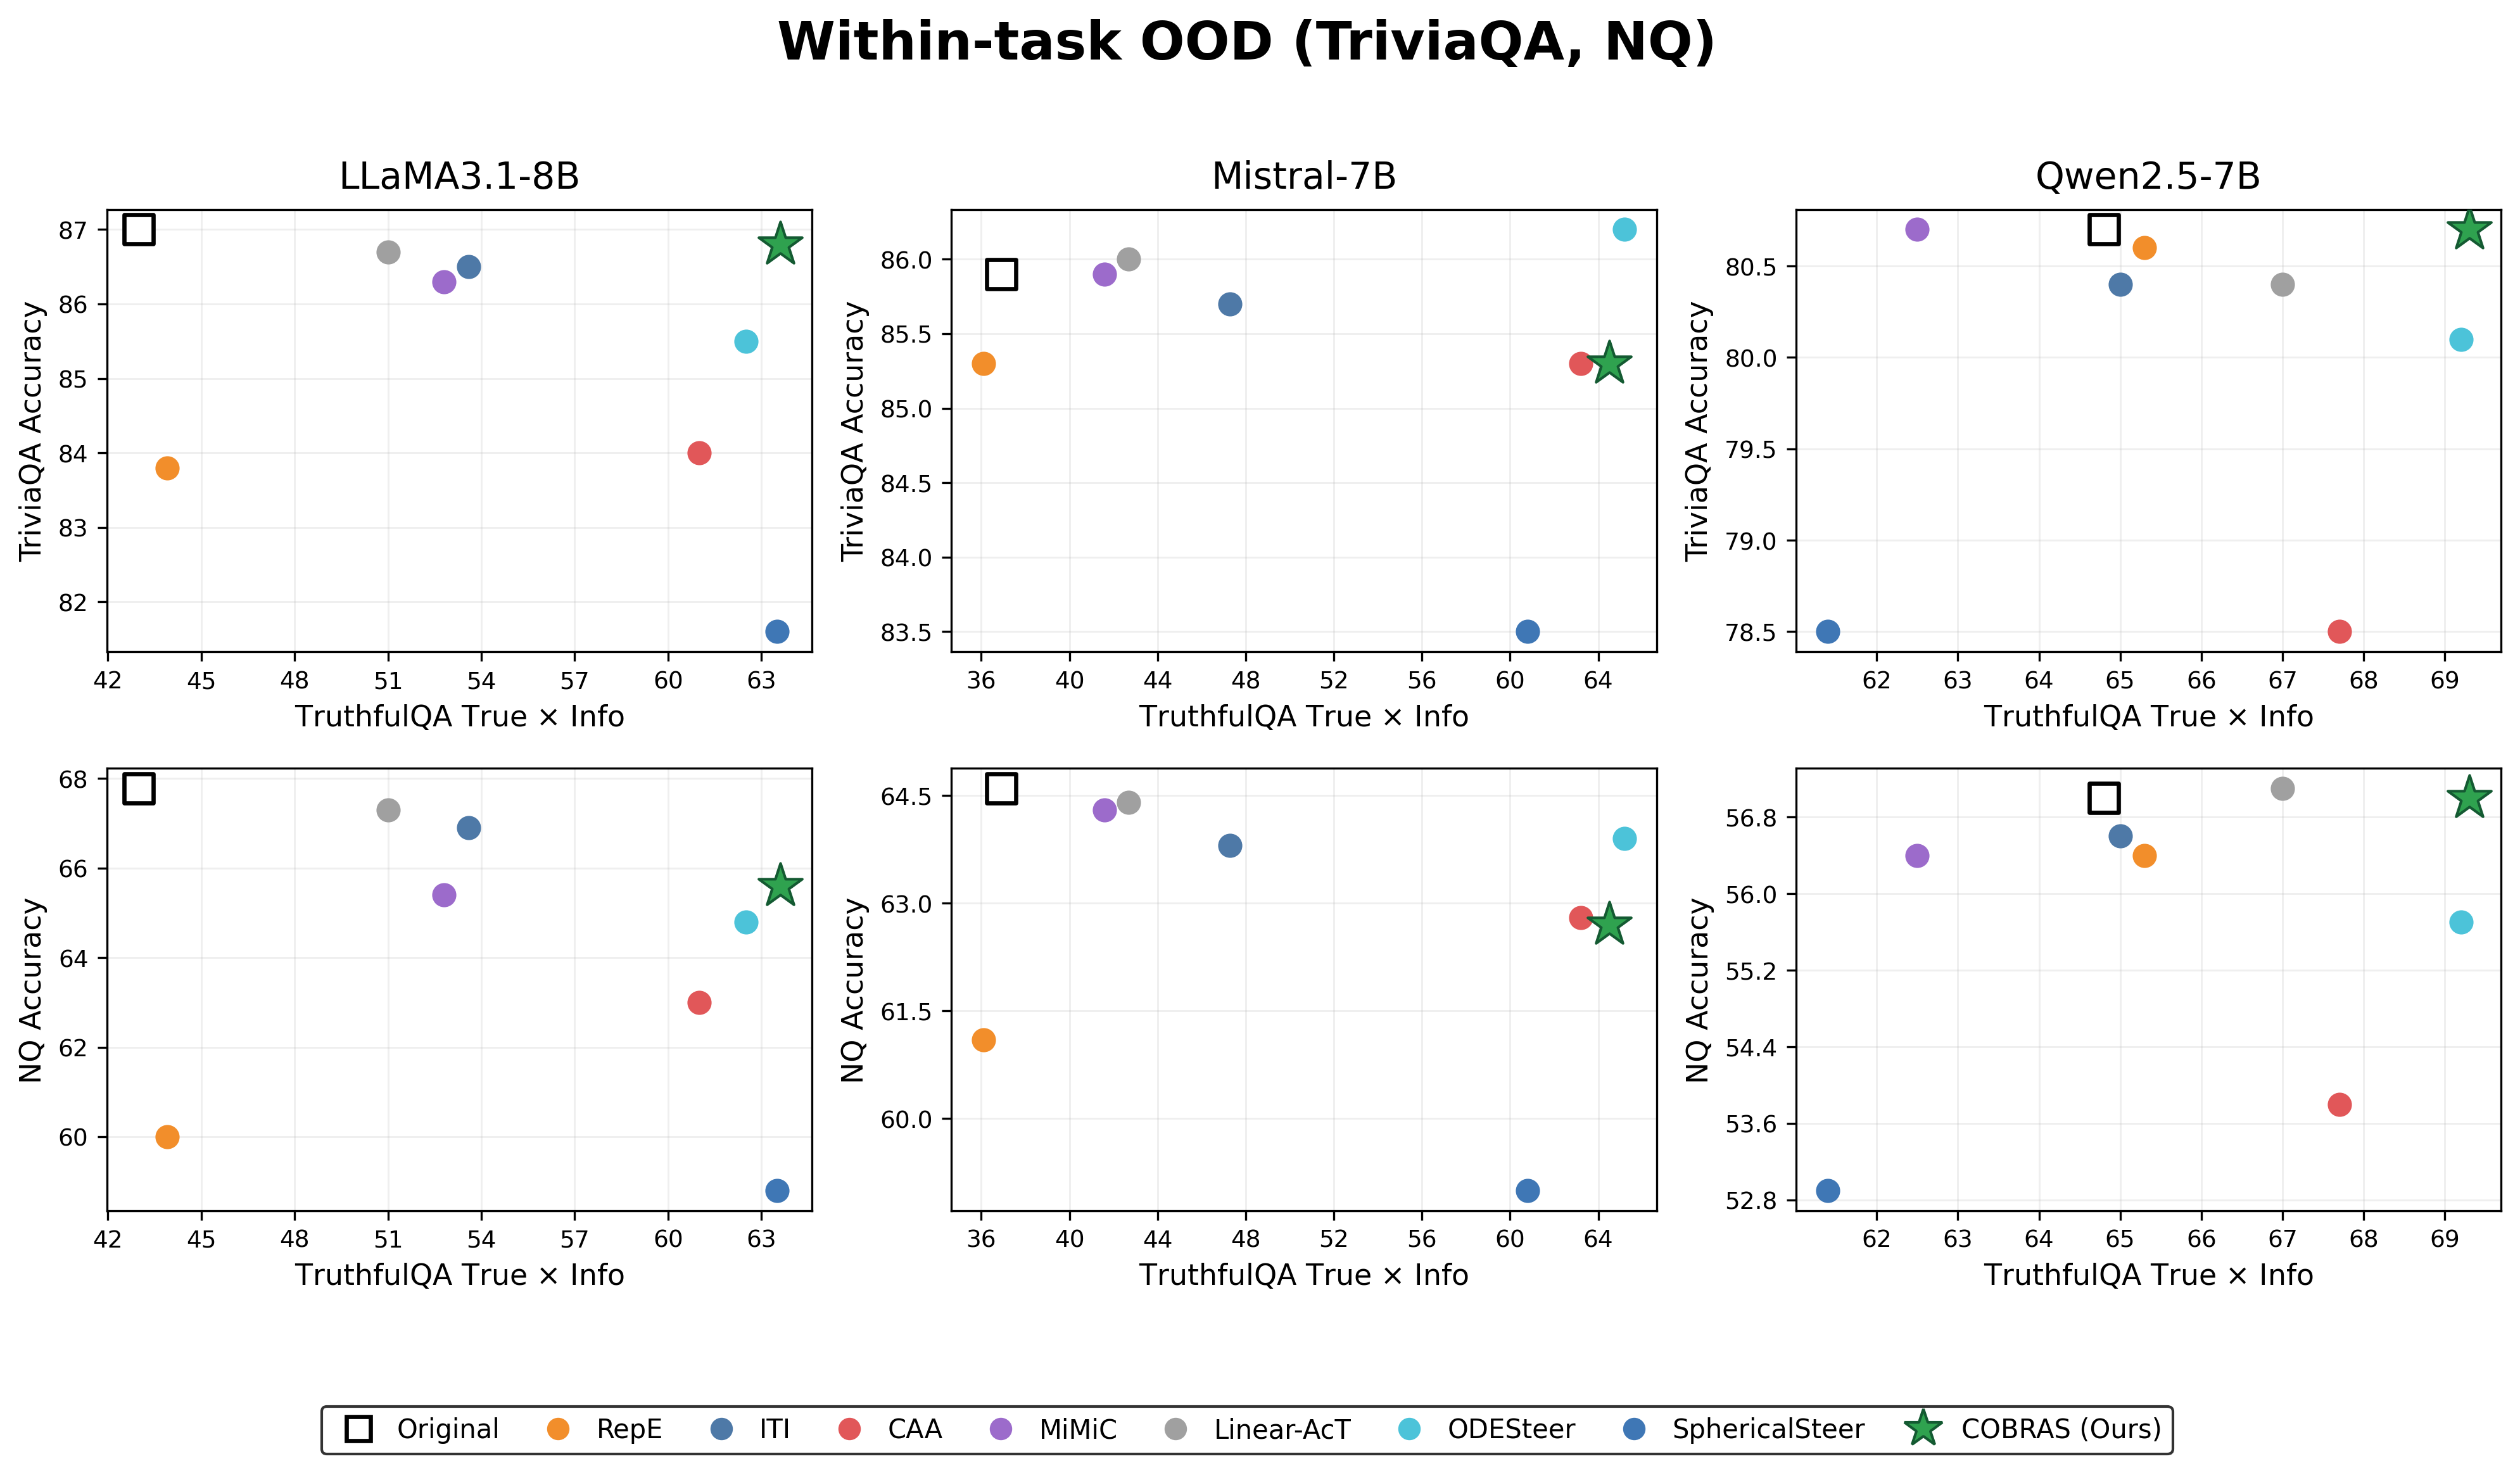
\includegraphics[width=\linewidth]{figures/within_task_ood1.png}
    \caption{Within-task OOD evaluation. Answer-ranking accuracy on TriviaQA~\citep{joshi2017triviaqa} and NQ~\citep{kwiatkowski2019natural} is plotted against TruthfulQA True$\times$Info. Falcon-7B is omitted due to its low unsteered performance.}
    \label{fig:within_task_ood}\vspace{-5mm}
\end{figure}

\noindent\textbf{RQ1: In-distribution steering performance.}~We first evaluate \Cobras in the standard in-distribution setting, where each steering method is trained and tested on the same task axis. We consider three representative alignment objectives: helpfulness on UltraFeedback, truthfulness on TruthfulQA, and detoxification on RealToxicityPrompts. Table~\ref{tab:main_results} reports results across four models.

\Cobras improves the primary metric over the unsteered model for all three tasks across models. On helpfulness, it achieves the highest mean UltraFeedback win rate for every model, improving over the original model by $+2.8$, $+7.1$, $+9.7$, and $+1.9$ absolute points on Falcon-7B, Mistral-7B, LLaMA3.1-8B, and Qwen2.5-7B, respectively. On truthfulness, it obtains the highest mean TruthfulQA True$\times$Info score across all four models, with especially large gains on Mistral-7B $(+29.5)$ and LLaMA3.1-8B $(+25.1)$. On detoxification, it reduces toxicity by approximately $41\%$--$54\%$ relative to the original models and has the lowest mean toxicity on three of four models. On Falcon-7B, CAA reduces toxicity further ($0.076$ versus $0.138$) but has substantially higher perplexity ($75.550$ versus $15.304$).
% Compared to prior steering baselines, \Cobras provides the most consistent gains across objectives. While some baselines perform well on individual tasks, they often introduce undesirable trade-offs, such as reduced informativeness on TruthfulQA or large perplexity increases on RealToxicityPrompts. In contrast, \Cobras improves the target alignment metrics while largely preserving generation quality, as reflected by competitive reward-model scores, informativeness, perplexity, and diversity. These results show that \Cobras is a strong and robust in-distribution steering method across helpfulness, truthfulness, and detoxification.

Compared to prior steering baselines, \Cobras delivers the most consistent gains across objectives. While other methods can perform well on individual tasks, they often trade off informativeness, perplexity, or diversity. In contrast, \Cobras improves target alignment metrics while largely preserving generation quality, making it a robust in-distribution steering method across helpfulness, truthfulness, and detoxification.

\noindent\textbf{RQ2: Performance under distribution shift.}~Activation steering can be brittle under distribution shift, with prior work showing that steering vectors may be unreliable in-distribution and can misgeneralize out-of-distribution ~\citep{tan2024analysing,braun2025understanding,korznikov2025rogue}. We therefore evaluate whether \Cobras improves TruthfulQA performance without degrading other capabilities by conducting experiments on both (i) within-task OOD and (ii) cross-task OOD, using the support gate in Eq.~\eqref{eq:gate} for \Cobras.


\noindent\textbf{Within-task OOD.}~In this experiment, we evaluate the performance of steering methods on two datasets, Natural Questions (NQ)~\cite{kwiatkowski2019natural} and TriviaQA~\cite{joshi2017triviaqa}, relevant to truthfulness by training only on TruthfulQA. Figure~\ref{fig:within_task_ood} plots OOD accuracy against TruthfulQA True$\times$Info; the ideal method appears in the upper-right, improving truthfulness while preserving OOD accuracy. While most methods move substantially along the TruthfulQA axis, their behavior on TriviaQA and NQ varies considerably, with some producing marked accuracy losses—most visibly on NQ. \Cobras shows a different pattern: across all three models, it attains the largest TruthfulQA improvements while keeping performance on both OOD datasets near the top of the corresponding plots. These results suggest that the gains from \Cobras are not limited to the training distribution and transfer with minimal disruption to closely related QA capabilities.

In this experiment, we evaluate the performance of steering methods on Natural Questions (NQ)~\cite{kwiatkowski2019natural} and TriviaQA~\cite{joshi2017triviaqa}, using steering learned exclusively from TruthfulQA. Figure~\ref{fig:within_task_ood} plots OOD answer-ranking accuracy against TruthfulQA True$\times$Info, where the upper-right region represents a favorable trade-off between in-distribution steering effectiveness and OOD capability retention. Several baselines achieve substantial TruthfulQA improvements but incur noticeable accuracy losses on NQ and TriviaQA, particularly SphericalSteer and CAA. In contrast, \Cobras achieves among the highest TruthfulQA scores while largely preserving OOD accuracy across all three models. On LLaMA3.1-8B and Qwen2.5-7B, \Cobras maintains performance close to the unsteered models, whereas on Mistral-7B, ODESteer provides slightly better OOD accuracy. Overall, these results indicate that \Cobras can improve in-distribution truthfulness metrics while retaining much of the models' factual question-answering capability under related distribution shifts.


\begin{figure}[t]
    \centering
    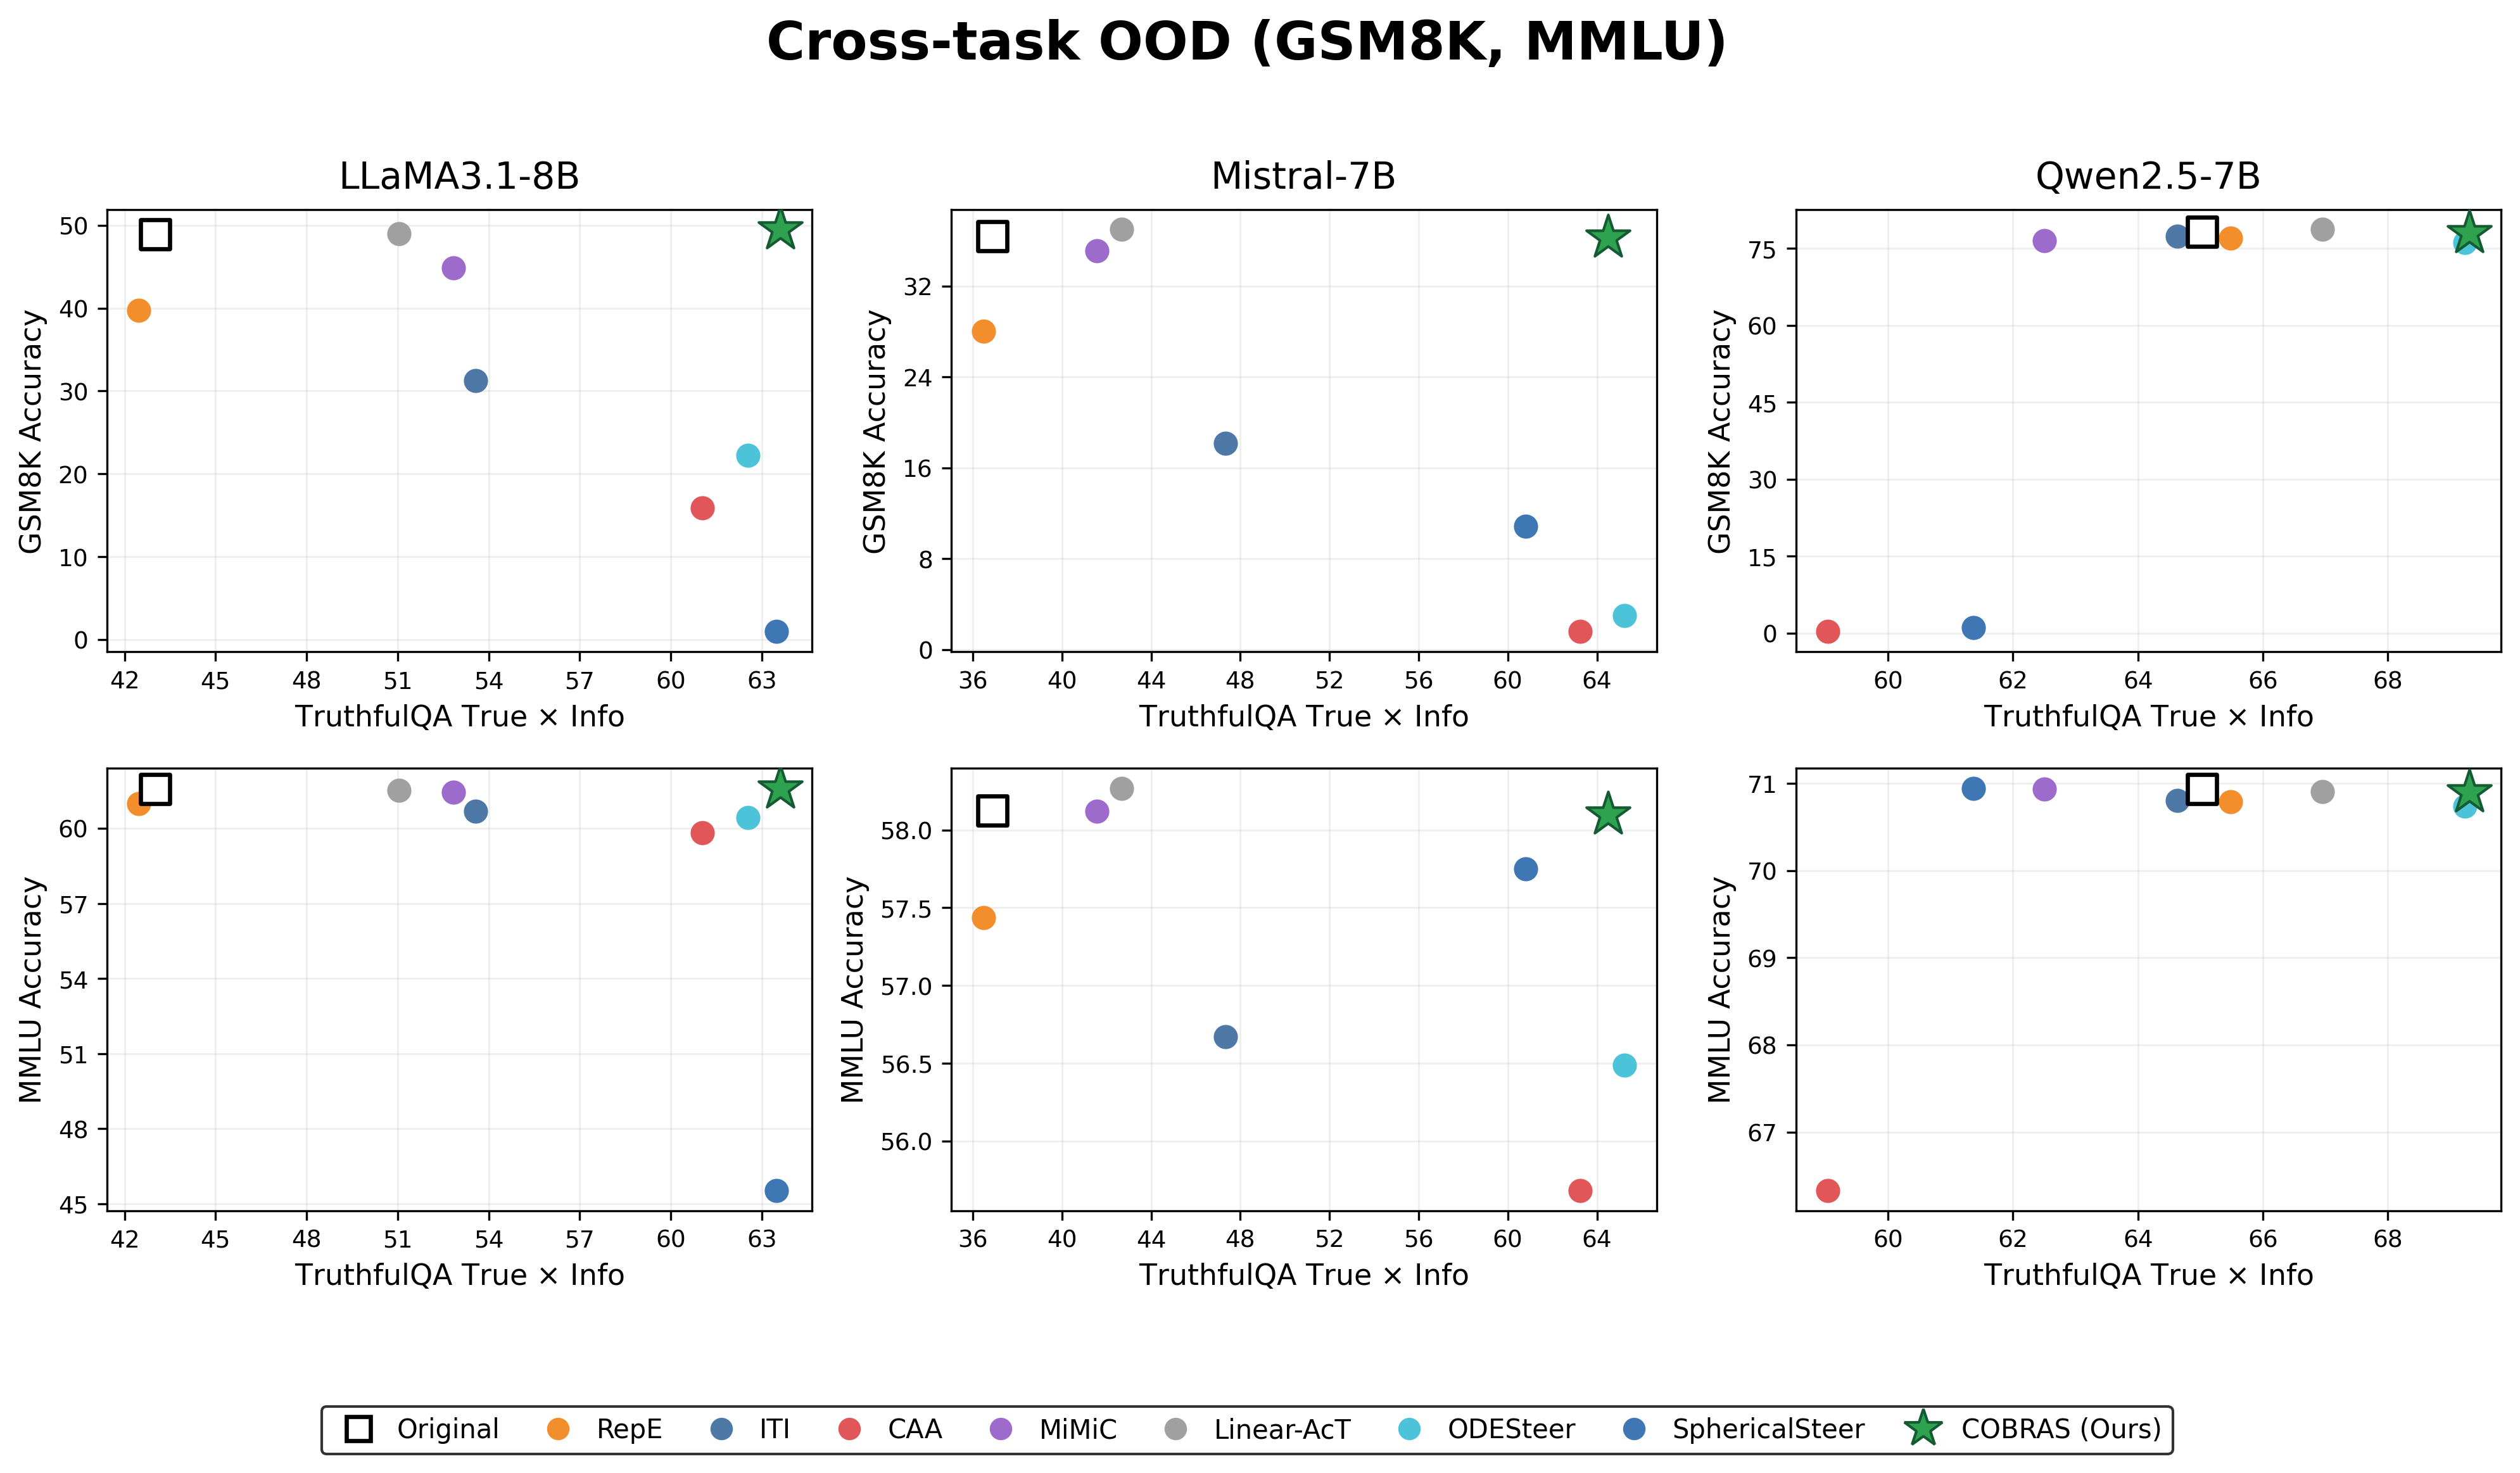
\includegraphics[width=\linewidth]{figures/cross_task_ood1.png}
    \caption{Performance of steering methods in Cross-task OOD: MMLU~\cite{hendrycks2020measuring} and GSM8K~\cite{cobbe2021gsm8k} performance. We skipped Falcon-7B because the original model's performance was low.}
    \label{fig:cross_task_ood}\vspace{-5mm}
\end{figure}

\noindent\textbf{Cross-task OOD.}~In this experiment, we train all steering methods on TruthfulQA and evaluate OOD performance on MMLU~\cite{hendrycks2020measuring} and GSM8K~\cite{cobbe2021gsm8k}. Figure~\ref{fig:cross_task_ood} plots OOD accuracy against TruthfulQA True$\times$Info; the ideal method appears in the upper-right, improving truthfulness while preserving OOD accuracy. Baselines show inconsistent trade-offs: several methods improve TruthfulQA but substantially reduce OOD performance, especially on GSM8K for LLaMA3.1-8B and Mistral-7B, and on MMLU for Mistral-7B. This suggests that some steering methods sacrifice general reasoning ability for in-distribution gains. By contrast, \Cobras consistently lies near the upper-right across all models and OOD benchmarks. It improves TruthfulQA over the original model while maintaining OOD accuracy close to, or above, the unsteered model, avoiding the severe GSM8K drops seen in several baselines. Overall, \Cobras achieves the most favorable trade-off between in-distribution steering effectiveness and OOD capability preservation.

\noindent\textbf{kNN gating across steering methods.}~We next test whether gating can also preserve OOD accuracy for other steering methods. On LLaMA3.1-8B, we compare CAA, ODESteer, SphericalSteer, and \Cobras fitted on TruthfulQA with and without a common kNN gate; for \Cobras, it replaces the support gate. Across all four methods, gating restores GSM8K and MMLU accuracy close to unsteered levels, at a cost of $1.7$--$4.0$ percentage points in TruthfulQA True$\times$Info (Table~\ref{tab:knn-external}, Appendix~\ref{apx:knn}). With this common gate, \Cobras retains the highest mean True$\times$Info ($63.6\%$ vs.\ $61.7\%$ for Spherical Steering), indicating that target-task gains still depend on the steering rule.


% \begin{figure}[!ht]
%     \centering
%     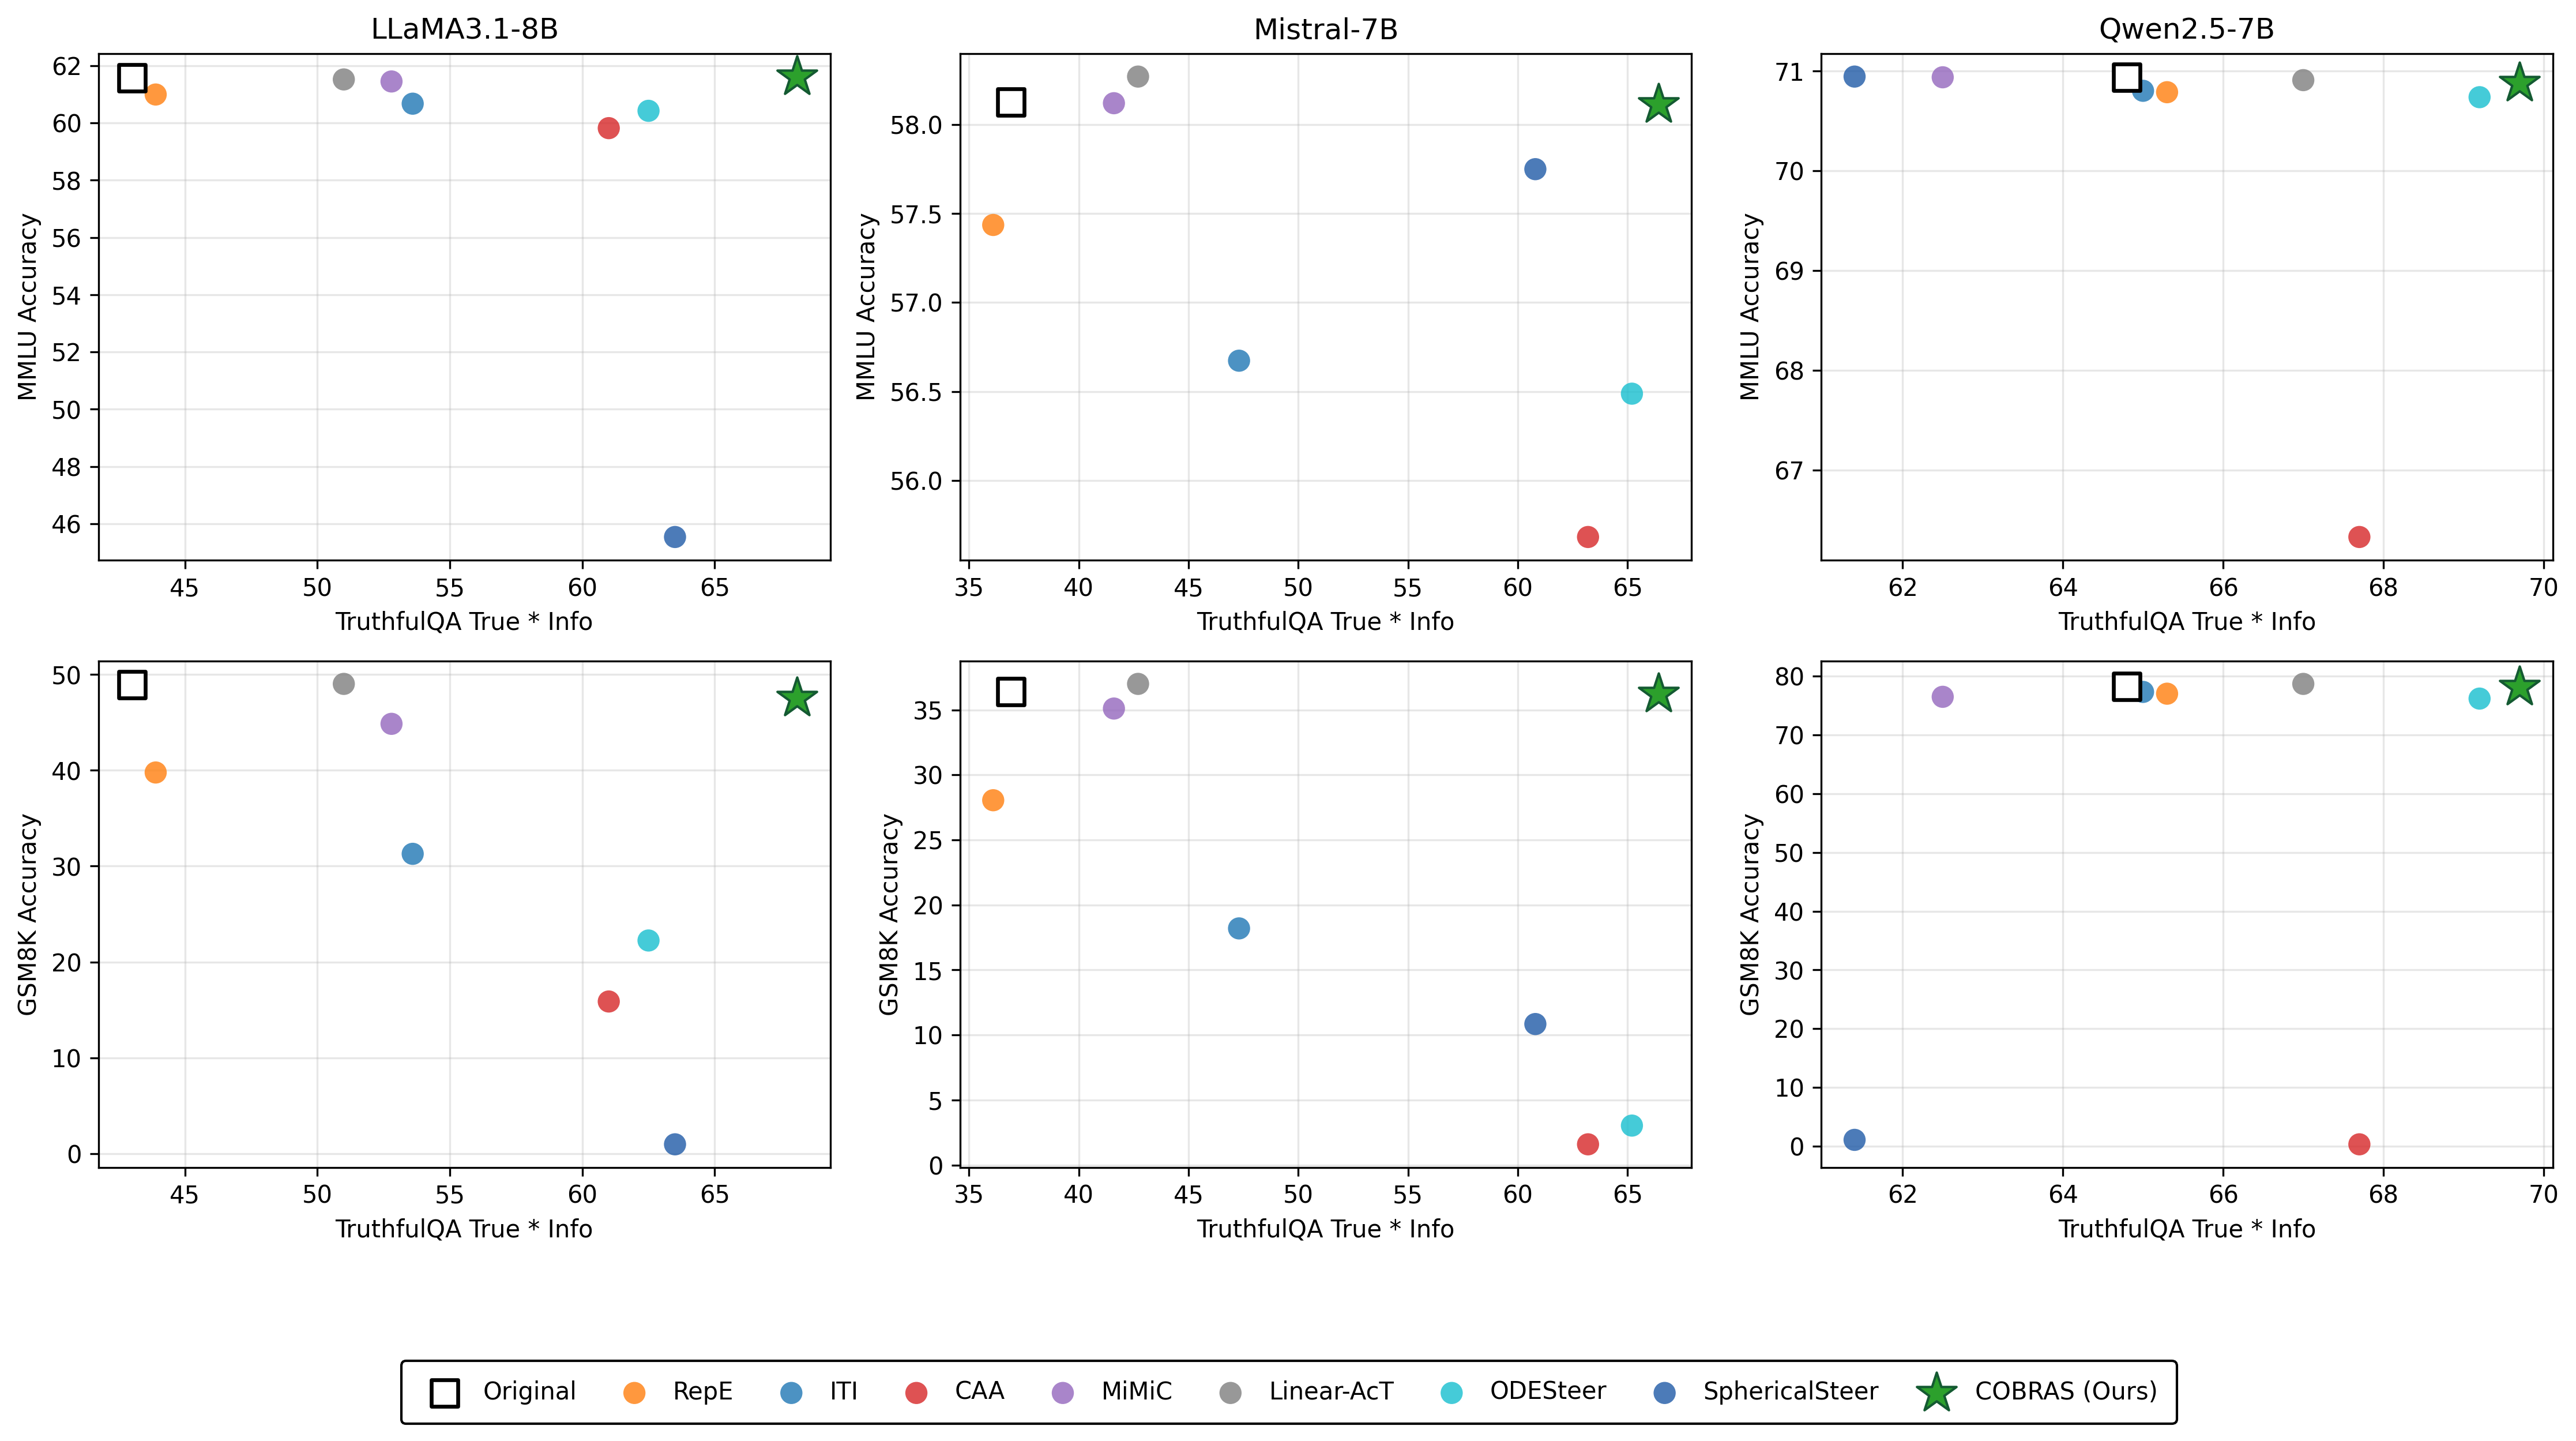
\includegraphics[width=\linewidth]{figures/tqa_vs_ood_absolute.png}
%     \caption{Performance of steering methods in OOD tasks: MMLU~\cite{hendrycks2020measuring} and GSM8K~\cite{cobbe2021gsm8k} performance. We skipped Falcon-7B because the original model's performance was low.}
%     \label{fig:ood}\vspace{-3mm}
% \end{figure}


% \paragraph{RQ3: Ablation of \Cobras Hyperparameters}
% We ablate two key hyperparameters of \Cobras, i) the abstention neighborhood size $K$, and ii) the abstention percentile. Further, ablation for Steering Strength is deferred to Appendix~\ref{appendix:cobras_vs_t}.


%\noindent\textbf{Effect of abstention parameters:} \Cobras uses an abstention rule to avoid steering inputs far from the training distribution. For each training example, we compute the distance to its $K$-th nearest neighbor and set the abstention threshold to a chosen percentile of these distances. At test time, \Cobras abstains from steering when an input's neighborhood distance exceeds this threshold. In-distribution inputs are expected to have nearby neighbors and therefore be steered, whereas OOD inputs should have larger distances and trigger abstention. Table~\ref{tab:abstain-results} evaluate this mechanism on LLaMA3.1-8B-Base and Mistral-7B-Base using TruthfulQA as the in-distribution task and GSM8K as the OOD task. Increasing the abstention percentile makes \Cobras steer more examples. This improves TruthfulQA True$\times$Info, but can reduce OOD accuracy, most notably for LLaMA3.1-8B-Base at the $99.5$th percentile. Increasing $K$ shows a similar trade-off: larger neighborhoods improve TruthfulQA, but can lower GSM8K accuracy, especially for LLaMA3.1-8B-Base. These results show that abstention helps balance effective in-distribution steering with preserving OOD capabilities.

\noindent{\textbf{RQ3: Ablations and computational cost.}}~We examine how each component of \Cobras affects its performance. On LLaMA3.1-8B, removing the support gate weakens OOD retention. Using Euclidean geometry instead of Riemannian geometry decreases performance on both in-distribution and OOD data, while removing the alignment coefficient reduces informativeness (Appendix~\ref{apx:component-ablations}). Coverage $p$ tunes the OOD trade-off (Appendix~\ref{apx:ood-gate}). Sweeps vary the integration horizon $T$, integration steps $K$, and vMF concentration $\kappa$ (Appendices~\ref{appendix:cobras_vs_t}--\ref{appendix:cobras_vs_kappa}). We also analyzed the computational overhead and potential mitigations: using $25\%$ of each contrastive dataset and $K=2$ lowers decoding overhead from $32\%$ to $7\%$ with a $1.8$-point True$\times$Info loss (Appendix~\ref{apx:computational-cost} for more details).



% Figure~\ref{fig:cobras_vs_t} shows the effect of varying the steering strength $T$ from $0.1$ to $1.0$ on TruthfulQA and UltraFeedback. On TruthfulQA, most models exhibit a clear non-monotonic trend: increasing $T$ initially improves True$\times$Info, but overly large values eventually degrade performance. LLaMA3.1-8B peaks around $T=0.6$, Mistral-7B around $T=0.7$, and Qwen2.5-7B around $T=0.4$, while Falcon-7B remains comparatively weaker and flatter before dropping sharply at high $T$. This suggests that moderate steering is sufficient for truthfulness, whereas excessive steering can overcorrect model behavior.\\
% On UltraFeedback, the effect of $T$ is more model-dependent. LLaMA3.1-8B maintains high win rate for moderate values of $T$ and peaks near $T=0.3$--$0.5$, while Falcon-7B remains relatively stable across the full range. In contrast, Mistral-7B and Qwen2.5-7B generally degrade as $T$ increases, indicating that stronger steering can harm preference-aligned generation quality. Across both datasets, these results motivate using a moderate steering strength, with the best values typically lying around $T=0.5$--$0.7$ for TruthfulQA and lower-to-moderate values for UltraFeedback.




% \begin{table}[ht]
%   \centering
%     \caption{Effect of varying the abstention percentile on LLaMA3.1-8B-Base and Mistral-7B-Base, with abstention neighborhood size fixed to $K=32$.}
%   \label{tab:abstain-percentile-results}
%     \resizebox{\linewidth}{!}{%
%       \begin{tabular}{ccccc}
%         \toprule
%         & \multicolumn{2}{c}{LLaMA3.1-8B-Base} & \multicolumn{2}{c}{Mistral-7B-Base} \\
%         \cmidrule(lr){2-3} \cmidrule(lr){4-5}
%         Abstain Percentile 
%         & TQA: T$\times$I (\%) 
%         & GSM8K: Accuracy (\%) 
%         & TQA: T$\times$I (\%) 
%         & GSM8K: Accuracy (\%) \\
%         \midrule
%         90.0  & 44.67 & 48.67 & 36.23 & 36.89 \\
%         95.0  & 54.83 & 48.90 & 37.08 & 36.31 \\
%         98.0  & 65.48 & 47.53 & 42.71 & 36.23 \\
%         99.5  & 69.15 & 11.59 & 59.48 & 35.53 \\
%         \bottomrule
%       \end{tabular}
%     }
% \end{table}

% \begin{table}[ht]
%   \centering
%   \caption{Effect of varying the abstention neighborhood size $K$ on LLaMA3.1-8B-Base and Mistral-7B-Base, with abstention percentile fixed to $98.0$.}
%   \label{tab:abstain-k-results}
%     \resizebox{\linewidth}{!}{%
%       \begin{tabular}{ccccc}
%         \toprule
%         & \multicolumn{2}{c}{LLaMA3.1-8B-Base} & \multicolumn{2}{c}{Mistral-7B-Base} \\
%         \cmidrule(lr){2-3} \cmidrule(lr){4-5}
%         Abstain $K$
%         & TQA: T$\times$I (\%) 
%         & GSM8K: Accuracy (\%) 
%         & TQA: T$\times$I (\%) 
%         & GSM8K: Accuracy (\%) \\
%         \midrule
%         32   & 65.48 & 47.53 & 42.71 & 36.23 \\
%         128  & 68.91 & 25.92 & 49.81 & 36.51 \\
%         256  & 69.40 & 15.08 & 52.50 & 36.90 \\
%         \bottomrule
%       \end{tabular}
%     }
% \end{table}


% REMOVED
% \begin{table}[ht]
%   \centering
%   \vspace{-2mm}
%   \caption{Effect of abstention parameters on LLaMA3.1-8B-Base and Mistral-7B-Base. Percentile ablations fix $K=32$, while $K$ ablations fix the abstention percentile to $98.0$.}
%   \label{tab:abstain-results}
%   \resizebox{\linewidth}{!}{%
%   % \small
%     \begin{tabular}{cccccc}
%       \toprule
%       \multirow{2}{*}{Ablation}
%       & \multirow{2}{*}{Value}
%       & \multicolumn{2}{c}{LLaMA3.1-8B-Base} 
%       & \multicolumn{2}{c}{Mistral-7B-Base} \\
%       \cmidrule(lr){3-4} \cmidrule(lr){5-6}
%       &
%       & TQA: T$\times$I (\%) ($\uparrow$)
%       & GSM8K: Acc. (\%) ($\uparrow$)
%       & TQA: T$\times$I (\%) ($\uparrow$) 
%       & GSM8K: Acc. (\%) ($\uparrow$)\\
%       \midrule

%       \multirow{4}{*}{Percentile}
%       & $90.0$  & 44.67 & 48.67 & 36.23 & 36.89 \\
%       & $95.0$  & 54.83 & 48.90 & 37.08 & 36.31 \\
%       & $98.0$  & 65.48 & 47.53 & 42.71 & 36.23 \\
%       & $99.5$  & 69.15 & 11.59 & 59.48 & 35.53 \\

%       \midrule

%       \multirow{3}{*}{$K$}
%       & $32$   & 65.48 & 47.53 & 42.71 & 36.23 \\
%       & $128$  & 68.91 & 25.92 & 49.81 & 36.51 \\
%       & $256$  & 69.40 & 15.08 & 52.50 & 36.90 \\

%       \bottomrule
%     \end{tabular}\vspace{-2mm}
%   }
% \end{table}

% \begin{table*}[!h]
% \label{tab:main_results}
% \centering
% \scriptsize
% \caption{Comparison of methods on multiple base models for helpfulness, truthfulness, and detoxification.\textcolor{red}{Arshan will update TQA , Ajay will update UF and Toxicity Eval}}
% \setlength{\tabcolsep}{3.5pt}
% \renewcommand{\arraystretch}{1.12}
% \resizebox{\textwidth}{!}{%
% \begin{tabular}{lc|ccc|ccc|ccc}
% \toprule
% \multirow{2}{*}{\textbf{Method}} & \multirow{2}{*}{\textbf{Model}} 
% & \multicolumn{3}{c|}{\textbf{Helpfulness} (\textit{UltraFeedback})}
% & \multicolumn{3}{c|}{\textbf{Truthfulness} (\textit{TruthfulQA})}
% & \multicolumn{3}{c}{\textbf{Detoxification} (\textit{Real Toxicity Prompts})} \\
% & 
% & Win (\%) $\uparrow$ & RM$_{\text{mean}}$ $\uparrow$ & RM$_{p90}$ $\uparrow$
% & T$\times$I (\%) $\uparrow$ & True (\%) $\uparrow$ & Info (\%) $\uparrow$
% & Toxic $\downarrow$ & PPL $\downarrow$ & Dist-2 $\uparrow$ \\
% \midrule

% Original & \multirow{10}{*}{\rotatebox[origin=c]{90}{LLaMA3.1-8B}}
% & 50.0 {\tiny $\pm$ 0.000} & -10.303 {\tiny $\pm$ 0.145} & -0.744 {\tiny $\pm$ 0.435} 
% & 43.0 {\tiny $\pm$ 1.496} & 45.1 {\tiny $\pm$ 1.309} & 97.6 {\tiny $\pm$ 0.628}
% & 0.218 {\tiny $\pm$ 0.002} & 18.562 {\tiny $\pm$ 0.107} & 0.992 {\tiny $\pm$ 0.001}  \\\midrule


% RepE &
% & 47.1 {\tiny $\pm$ 1.050} & -10.763 {\tiny $\pm$ 0.295} & -1.356 {\tiny $\pm$ 0.378} 
% & 43.9 {\tiny $\pm$ 1.041} & 46.2 {\tiny $\pm$ 0.989} & 97.4 {\tiny $\pm$ 0.187}
% & 0.195 {\tiny $\pm$ 0.003} & 19.101 {\tiny $\pm$ 0.496} & 0.991 {\tiny $\pm$ 0.001} \\

% ITI &
% & 51.5 {\tiny $\pm$ 2.026} & -10.138 {\tiny $\pm$ 0.232} & -0.739 {\tiny $\pm$ 0.611} 
% & 53.6 {\tiny $\pm$ 1.055} & 57.3 {\tiny $\pm$ 0.902} & 95.8 {\tiny $\pm$ 0.374}
% & 0.190 {\tiny $\pm$ 0.011} & 18.698 {\tiny $\pm$ 0.377} & 0.990 {\tiny $\pm$ 0.002} \\

% CAA &
% & 50.9 {\tiny $\pm$ 0.874} & -9.966 {\tiny $\pm$ 0.132} & -0.628 {\tiny $\pm$ 0.380} 
% & 61.0 {\tiny $\pm$ 2.020} & 68.1 {\tiny $\pm$ 2.221} & 92.6 {\tiny $\pm$ 0.495}
% & 0.152 {\tiny $\pm$ 0.005} & 19.647 {\tiny $\pm$ 0.349} & 0.992 {\tiny $\pm$ 0.001} \\

% MiMiC &
% & 54.9 {\tiny $\pm$ 1.905} & -9.713 {\tiny $\pm$ 0.175} & -0.549 {\tiny $\pm$ 0.112} 
% & 52.8 {\tiny $\pm$ 1.041} & 60.1 {\tiny $\pm$ 0.430} & 92.0 {\tiny $\pm$ 0.612}
% & 0.198 {\tiny $\pm$ 0.010} & 18.667 {\tiny $\pm$ 0.311} & 0.991 {\tiny $\pm$ 0.001} \\

% Linear-AcT &
% & 52.5 {\tiny $\pm$ 2.203} & -9.944 {\tiny $\pm$ 0.469} & -0.411 {\tiny $\pm$ 0.654}
% & 51.0 {\tiny $\pm$ 1.484} & 53.1 {\tiny $\pm$ 1.683} & 97.8 {\tiny $\pm$ 0.187}
% & 0.199 {\tiny $\pm$ 0.014} & 18.521 {\tiny $\pm$ 0.333} & 0.991 {\tiny $\pm$ 0.001} \\

% ODESteer &
% & 56.3 {\tiny $\pm$ 0.896} & -8.280 {\tiny $\pm$ 0.316} & 1.206 {\tiny $\pm$ 0.441} & 62.5 {\tiny $\pm$ 2.570} & 67.3 {\tiny $\pm$ 2.544} & 95.1 {\tiny $\pm$ 0.441}
% & 0.124 {\tiny $\pm$ 0.002} & 19.831 {\tiny $\pm$ 0.224} & 0.993 {\tiny $\pm$ 0.000}  \\

% SphericalSteer &
% & 52.3 {\tiny $\pm$ 1.790} & -9.434 {\tiny $\pm$ 0.304} & -0.633 {\tiny $\pm$ 0.837} & 63.5 {\tiny $\pm$ 0.902} & 86.9 {\tiny $\pm$ 2.389} & 76.0 {\tiny $\pm$ 1.504} 
% & 0.123 {\tiny $\pm$ 0.010} & 23.039 {\tiny $\pm$ 0.274} & 0.993 {\tiny $\pm$ 0.000} \\

% \midrule

% \textbf{COBRAS (Ours)} &
% & \textbf{59.7} {\tiny $\pm$ 1.610}  & -8.109 {\tiny $\pm$ 0.283}  &  0.800 {\tiny $\pm$ 0.120}
% & \textbf{68.1} {\tiny $\pm$ 1.343} & 82.8 {\tiny $\pm$ 0.308} & 84.9 {\tiny $\pm$ 1.168}
% & 0.107 {\tiny $\pm$ 0.004} & 20.083 {\tiny $\pm$ 0.184} & 0.992 {\tiny $\pm$ 0.000} \\

% \midrule
% \midrule
% Original & \multirow{10}{*}{\rotatebox[origin=c]{90}{Falcon-7B}}
% & 50.0 {\tiny $\pm$ 0.000} & -12.642 {\tiny $\pm$ 0.162} & -2.705 {\tiny $\pm$ 0.171} 
% & 29.1 {\tiny $\pm$ 0.919} & 32.1 {\tiny $\pm$ 0.951} & 96.5 {\tiny $\pm$ 0.283} 
% & 0.255 {\tiny $\pm$ 0.004} & 15.358 {\tiny $\pm$ 0.449} & 0.946 {\tiny $\pm$ 0.003} \\\midrule



% RepE &
% & 50.2 {\tiny $\pm$ 0.981} & -12.711 {\tiny $\pm$ 0.270} & -2.680 {\tiny $\pm$ 0.099} 
% & 28.7 {\tiny $\pm$ 1.069} & 31.7 {\tiny $\pm$ 0.982} & 96.6 {\tiny $\pm$ 0.308} 
% & 0.232 {\tiny $\pm$ 0.010} & 15.371 {\tiny $\pm$ 0.178} & 0.941 {\tiny $\pm$ 0.003}  \\

% ITI &
% & 49.0 {\tiny $\pm$ 1.358} & -12.789 {\tiny $\pm$ 0.221} & -2.866 {\tiny $\pm$ 0.134} 
% & 32.8 {\tiny $\pm$ 0.616} & 36.8 {\tiny $\pm$ 0.738} & 95.5 {\tiny $\pm$ 0.393}
% & 0.239 {\tiny $\pm$ 0.004} & 15.707 {\tiny $\pm$ 0.346} & 0.941 {\tiny $\pm$ 0.005} \\

% CAA &
% & 49.9 {\tiny $\pm$ 2.346} & -12.540 {\tiny $\pm$ 0.226} & -2.260 {\tiny $\pm$ 0.410} 
% & 37.9 {\tiny $\pm$ 1.495} & 42.0 {\tiny $\pm$ 1.905} & 95.4 {\tiny $\pm$ 0.494}
% & 0.076 {\tiny $\pm$ 0.007} & 75.550 {\tiny $\pm$ 9.063} & 0.852 {\tiny $\pm$ 0.002} \\

% MiMiC &
% & 50.7 {\tiny $\pm$ 1.350} & -12.751 {\tiny $\pm$ 0.136} & -2.678 {\tiny $\pm$ 0.213} 
% & 32.9 {\tiny $\pm$ 0.764} & 43.3 {\tiny $\pm$ 0.374} & 88.3 {\tiny $\pm$ 0.927} 
% & 0.240 {\tiny $\pm$ 0.009} & 15.026 {\tiny $\pm$ 0.258} & 0.941 {\tiny $\pm$ 0.004}  \\

% Linear-AcT &
% & 50.8 {\tiny $\pm$ 1.300} & -12.412 {\tiny $\pm$ 0.205} & -2.534 {\tiny $\pm$ 0.309} 
% & 40.0 {\tiny $\pm$ 0.561} & 44.3 {\tiny $\pm$ 0.534} & 95.0 {\tiny $\pm$ 0.212}
% & 0.240 {\tiny $\pm$ 0.003} & 16.113 {\tiny $\pm$ 0.206} & 0.947 {\tiny $\pm$ 0.002} \\


% ODESteer &
% & 49.7 {\tiny $\pm$ 1.210} & -12.446 {\tiny $\pm$ 0.050} & -2.806 {\tiny $\pm$ 0.207} 
% & 32.1 {\tiny $\pm$ 0.674} & 35.4 {\tiny $\pm$ 0.534} & 96.2 {\tiny $\pm$ 0.441} 
% & 0.188 {\tiny $\pm$ 0.006} & 15.709 {\tiny $\pm$ 0.405} & 0.940 {\tiny $\pm$ 0.002} \\

% SphericalSteer &
% & 49.5 {\tiny $\pm$ 2.255} & -12.495 {\tiny $\pm$ 0.120} & -3.108 {\tiny $\pm$ 0.244} 
% & 37.7 {\tiny $\pm$ 1.354} & 62.9 {\tiny $\pm$ 1.469} & 71.6 {\tiny $\pm$ 1.534} 
% & 0.147 {\tiny $\pm$ 0.011} & 21.542 {\tiny $\pm$ 1.543} & 0.924 {\tiny $\pm$ 0.008} \\

% \midrule
% \textbf{COBRAS (Ours)} &
% & \textbf{52.8} {\tiny $\pm$ 2.628}  &  -12.24 {\tiny $\pm$ 0.336}  & -2.60 {\tiny $\pm$ 0.121}  
% & \textbf{40.3} {\tiny $\pm$ 1.390} & 45.5 {\tiny $\pm$ 2.124} & 93.4 {\tiny $\pm$ 1.379}
% & 0.138 {\tiny $\pm$ 0.012} & 15.304 {\tiny $\pm$ 0.591} & 0.942 {\tiny $\pm$ 0.005} \\

% \midrule
% \midrule
% Original & \multirow{10}{*}{\rotatebox[origin=c]{90}{Mistral-7B}}
% & 50.0 {\tiny $\pm$ 0.000} & -11.063 {\tiny $\pm$ 0.377} & -0.469 {\tiny $\pm$ 0.752} 
% & 36.9 {\tiny $\pm$ 0.616} & 41.7 {\tiny $\pm$ 0.764} & 94.8 {\tiny $\pm$ 0.463} 
% & 0.207 {\tiny $\pm$ 0.008} & 18.542 {\tiny $\pm$ 0.498} & 0.990 {\tiny $\pm$ 0.001} \\\midrule


% RepE &
% & 45.3 {\tiny $\pm$ 2.237} & -11.981 {\tiny $\pm$ 0.377} & -1.622 {\tiny $\pm$ 0.423} 
% & 36.1 {\tiny $\pm$ 1.055} & 42.0 {\tiny $\pm$ 0.674} & 93.9 {\tiny $\pm$ 0.490} 
% & 0.218 {\tiny $\pm$ 0.004} & 76.065 {\tiny $\pm$ 1.734} & 0.969 {\tiny $\pm$ 0.001}  \\

% ITI &
% & 48.8 {\tiny $\pm$ 0.611} & -11.116 {\tiny $\pm$ 0.310} & -1.229 {\tiny $\pm$ 0.311} 
% & 47.3 {\tiny $\pm$ 1.952} & 54.2 {\tiny $\pm$ 1.616} & 92.6 {\tiny $\pm$ 1.041}
% & 0.181 {\tiny $\pm$ 0.013} & 18.956 {\tiny $\pm$ 0.170} & 0.989 {\tiny $\pm$ 0.000} \\

% CAA &
% & 53.7 {\tiny $\pm$ 4.636} & -10.424 {\tiny $\pm$ 0.144} & -0.601 {\tiny $\pm$ 0.439} 
% & 63.2 {\tiny $\pm$ 0.989} & 74.7 {\tiny $\pm$ 0.212} & 88.2 {\tiny $\pm$ 1.278}
% & 0.167 {\tiny $\pm$ 0.011} & 18.912 {\tiny $\pm$ 0.281} & 0.991 {\tiny $\pm$ 0.001}  \\

% MiMiC &
% & 48.5 {\tiny $\pm$ 2.751} & -11.511 {\tiny $\pm$ 0.324} & -0.676 {\tiny $\pm$ 0.535} 
% & 41.6 {\tiny $\pm$ 1.019} & 50.2 {\tiny $\pm$ 2.124} & 91.2 {\tiny $\pm$ 1.176}
% & 0.192 {\tiny $\pm$ 0.010} & 18.922 {\tiny $\pm$ 0.781} & 0.989 {\tiny $\pm$ 0.001}  \\


% Linear-AcT &
% & 53.0 {\tiny $\pm$ 4.996} & -10.448 {\tiny $\pm$ 0.191} & -0.139 {\tiny $\pm$ 0.544} 
% & 42.7 {\tiny $\pm$ 0.796} & 48.4 {\tiny $\pm$ 0.738} & 94.0 {\tiny $\pm$ 0.141} 
% & 0.189 {\tiny $\pm$ 0.009} & 18.784 {\tiny $\pm$ 0.320} & 0.990 {\tiny $\pm$ 0.001}  \\

% ODESteer &
% & 54.8 {\tiny $\pm$ 3.946} & -10.951 {\tiny $\pm$ 0.275} & -0.622 {\tiny $\pm$ 0.041}
% & 65.2 {\tiny $\pm$ 1.619} & 73.9 {\tiny $\pm$ 1.443} & 91.1 {\tiny $\pm$ 0.141}
% & 0.101 {\tiny $\pm$ 0.008} & 21.081 {\tiny $\pm$ 0.156} & 0.993 {\tiny $\pm$ 0.001} \\

% SphericalSteer &
% & 50.3 {\tiny $\pm$ 2.948} & -11.005 {\tiny $\pm$ 0.126} & -1.958 {\tiny $\pm$ 0.337} 
% & 60.8 {\tiny $\pm$ 1.630} & 76.6 {\tiny $\pm$ 1.324} & 83.7 {\tiny $\pm$ 0.510} 
% & 0.099 {\tiny $\pm$ 0.005} & 21.295 {\tiny $\pm$ 0.122} & 0.990 {\tiny $\pm$ 0.001} \\

% \midrule
% \textbf{COBRAS (Ours)} &
% & \textbf{57.1} {\tiny $\pm$ 3.253} & -10.261 {\tiny $\pm$ 0.163} & -0.157 {\tiny $\pm$ 0.621} 
% &  \textbf{66.4} {\tiny $\pm$ 1.901} & 85.2 {\tiny $\pm$ 0.972} & 80.3 {\tiny $\pm$ 0.982}
% & 0.096 {\tiny $\pm$ 0.006} & 20.631 {\tiny $\pm$ 0.330} & 0.992 {\tiny $\pm$ 0.001}  \\

% \midrule
% \midrule
% Original & \multirow{10}{*}{\rotatebox[origin=c]{90}{Qwen2.5-7B}}
% & 50.0 {\tiny $\pm$ 0.000} & -6.006 {\tiny $\pm$ 0.208} & 4.384 {\tiny $\pm$ 0.378} 
% & 64.8 {\tiny $\pm$ 0.707} & 78.3 {\tiny $\pm$ 0.578} & 86.4 {\tiny $\pm$ 0.764} 
% & 0.194 {\tiny $\pm$ 0.001} & 22.166 {\tiny $\pm$ 0.369} & 0.989 {\tiny $\pm$ 0.001}  \\\midrule


% RepE &
% & 48.8 {\tiny $\pm$ 0.300} & -6.011 {\tiny $\pm$ 0.202} & 4.504 {\tiny $\pm$ 0.271} 
% & 65.3 {\tiny $\pm$ 1.429} & 78.7 {\tiny $\pm$ 0.927} & 86.5 {\tiny $\pm$ 1.111} 
% & 0.196 {\tiny $\pm$ 0.002} & 22.620 {\tiny $\pm$ 0.681} & 0.990 {\tiny $\pm$ 0.000} \\

% ITI &
% & 49.9 {\tiny $\pm$ 1.054} & -6.034 {\tiny $\pm$ 0.373} & 4.349 {\tiny $\pm$ 0.408} 
% & 65.0 {\tiny $\pm$ 0.374} & 78.7 {\tiny $\pm$ 0.956} & 86.0 {\tiny $\pm$ 0.857} 
% & 0.184 {\tiny $\pm$ 0.005} & 22.617 {\tiny $\pm$ 0.895} & 0.990 {\tiny $\pm$ 0.001} \\

% CAA &
% & 50.0 {\tiny $\pm$ 1.587} & -5.957 {\tiny $\pm$ 0.072} & 4.659 {\tiny $\pm$ 0.312} 
% & 67.7 {\tiny $\pm$ 2.093} & 81.2 {\tiny $\pm$ 1.111} & 86.4 {\tiny $\pm$ 1.534} 
% & 0.114 {\tiny $\pm$ 0.005} & 28.218 {\tiny $\pm$ 1.014} & 0.982 {\tiny $\pm$ 0.002}  \\

% MiMiC &
% & 50.2 {\tiny $\pm$ 1.023 } & -5.980 {\tiny $\pm$ 0.133} & 4.753 {\tiny $\pm$ 0.312}  
% & 62.5 {\tiny $\pm$ 1.097} & 82.9 {\tiny $\pm$ 0.283} & 79.0 {\tiny $\pm$ 1.026} 
% & 0.176 {\tiny $\pm$ 0.005} & 21.233 {\tiny $\pm$ 0.363} & 0.989 {\tiny $\pm$ 0.002}  \\

% Linear-AcT &
% & 50.4 {\tiny $\pm$ 1.747} & -6.017 {\tiny $\pm$ 0.111} & 4.788 {\tiny $\pm$ 0.499} 
% & 67.0 {\tiny $\pm$ 1.168} & 79.8 {\tiny $\pm$ 1.205} & 87.0 {\tiny $\pm$ 1.046} 
% & 0.181 {\tiny $\pm$ 0.004} & 22.643 {\tiny $\pm$ 0.876} & 0.990 {\tiny $\pm$ 0.001} \\

% ODESteer &
% & 50.7 {\tiny $\pm$ 1.222} & -5.995 {\tiny $\pm$ 0.095} & 4.738 {\tiny $\pm$ 0.175} 
% & 69.2 {\tiny $\pm$ 1.434} & 82.2 {\tiny $\pm$ 1.460} & 86.7 {\tiny $\pm$ 2.145}
% & 0.170 {\tiny $\pm$ 0.004} & 22.310 {\tiny $\pm$ 0.565} & 0.990 {\tiny $\pm$ 0.002}  \\

% SphericalSteer &
% & 43.6 {\tiny $\pm$ 1.644} & -7.203 {\tiny $\pm$ 0.208} & 4.309 {\tiny $\pm$ 0.192} 
% & 61.4 {\tiny $\pm$ 2.086} & 82.9 {\tiny $\pm$ 1.874} & 77.6 {\tiny $\pm$ 1.067} 
% & 0.129 {\tiny $\pm$ 0.007} & 68.485 {\tiny $\pm$ 2.191} & 0.942 {\tiny $\pm$ 0.008} \\

% \midrule
% \textbf{COBRAS (Ours)} &
% & \textbf{51.9} {\tiny $\pm$ 1.616} &   -5.755 { \tiny$\pm$ 0.419} &    5.162 {\tiny $\pm$ 0.746}
% &  \textbf{69.7} {\tiny $\pm$ 0.495} & 83.3 {\tiny $\pm$ 0.430} & 86.8 {\tiny $\pm$ 0.141}
% & 0.119 {\tiny $\pm$ 0.006} & 23.786 {\tiny $\pm$ 0.625} & 0.985 {\tiny $\pm$ 0.003} \\

% \bottomrule
% \end{tabular}%
% }
% \label{tab:main_comparison}
% \end{table*}







% \begin{table*}[!h]
% \label{tab:main_results}
% \centering
% \scriptsize
% \caption{Comparison of methods on multiple base models for helpfulness, truthfulness, and detoxification.\textcolor{red}{Arshan will update TQA , Ajay will update UF and Toxicity Eval}}
% \setlength{\tabcolsep}{3.5pt}
% \renewcommand{\arraystretch}{1.12}
% \resizebox{\textwidth}{!}{%
% \begin{tabular}{lc|ccc|ccc|ccc}
% \toprule
% \multirow{2}{*}{\textbf{Method}} & \multirow{2}{*}{\textbf{Model}}  & \multicolumn{3}{c|}{\textbf{Helpfulness} (\textit{UltraFeedback})} & \multicolumn{3}{c|}{\textbf{Truthfulness} (\textit{TruthfulQA})} & \multicolumn{3}{c}{\textbf{Detoxification} (\textit{Real Toxicity Prompts})} \\
% \cline{3-5}
%  &  & RM$_{\text{mean}}$ $\uparrow$ & RM$_{p90}$ $\uparrow$ & Win (\%) $\uparrow$ & True (\%) $\uparrow$ & Info (\%) $\uparrow$ & T$\times$I (\%) $\uparrow$ & PPL $\downarrow$ & Dist-2 $\uparrow$ & Toxic $\downarrow$ \\
% \midrule

\vspace{-1mm}\section{Conclusion}
\label{sec:conclusion}
By bridging the gap between heuristic methods and the rigorous optimization framework of the Schr\"{o}dinger Bridge, this paper provides the first principled derivation of the log-density-ratio steering objective for activation steering. Experiments across four models and three alignment axes show that \Cobras consistently outperforms baselines in-distribution while preserving OOD performance (commonly seen in fixed-direction steering methods), thanks to its query-adaptive nature. \textcolor{blue}{The theoretical reduction is limited to a shared fixed bandwidth and does not establish optimality of the adaptive steering field at finite transport scale.} Limitations include the $\mathcal{O}(N_+ \cdot N_-)$ cost of pairwise geodesic distances and Sinkhorn, which may be prohibitive for very large contrastive sets, and the reliance on a fixed spherical geometry that may not hold for all architectures or layers. Promising future directions include hierarchical transport solvers to reduce computational overhead and extending the framework to learned or more general Riemannian manifolds.



%%%%%%%%%%%%%%%%%%%%%%%


\clearpage

% NeurIPS requires a funding and competing-interests disclosure in the camera-ready version,
% placed in this unnumbered section (it does not count toward the page limit). Uncomment and fill in.
\begin{ack}
This research is supported in part by
\end{ack}

%%%%%%%%%%%%%%%%%%%%% References %%%%%%%%%%%%%%%%%%%%%
\bibliography{ref}
\bibliographystyle{plain}

%%%%%%%%%%%%%%%%%%%%%%%%%%%%%%%%%%%%%%%%%%%%%%%%%%%%%%%%%%%%
\clearpage
\appendix
\section{Activation Steering Methods as Log-Density-Ratio Flows}
\label{apx:ldr-formalize}

Let $\pplus$ and $\pminus$ be densities on a manifold $\mathcal{M}$ describing the desired and undesired activation populations $\mathcal{D}^{+}$ and $\mathcal{D}^{-}$, and let a steering map carry a query activation along the flow
\begin{equation}
d\boldsymbol{x}_{t}
= \nabla_{\mathcal{M}}\log\frac{\pplus(\boldsymbol{x}_{t})}{\pminus(\boldsymbol{x}_{t})}\,dt,
\qquad \boldsymbol{x}_{0}=\hquery,
\label{eq:global-flow}
\end{equation}
discretized into $K$ Euler steps over a unit interval, with the distance traveled fixed by a per-method step size. We write $\Sph$ for the radius-$R$ sphere of Section~\ref{sec:bg}, on which the initial condition is the projection $\boldsymbol{x}_{0}=R\,\hquery/\lVert\hquery\rVert$. SS and HPR are stated on the unit sphere and differ from the radius-$R$ convention only by the rescaling $\boldsymbol{x}\mapsto R\boldsymbol{x}$.

Three choices place a steering method inside the family of Eq.~\eqref{eq:global-flow}: the manifold $\mathcal{M}$ on which the gradient is taken, the number of steps $K$, and the model that supplies the pair $(\pplus,\pminus)$. Each entry below is a reading rather than a re-derivation: we choose the density pair whose log-ratio gradient reproduces a method's published update and read off the assumptions the pair encodes, so what the reading exhibits is what a method implicitly assumes, not what its authors derived.\footnote{\citet{zhaoodesteer} give a related reading of several steering methods with $\mathcal{M}$ fixed to $\mathbb{R}^{d}$, and treating $\mathcal{M}$ as one of the three choices extends the same reading to the spherical methods SS and HPR.} The reading is exact for CAA, SS, ITI and HPR, whose published updates are the single Euler step of Eq.~\eqref{eq:global-flow} under the stated densities, and for ODESteer the log-ratio is itself the fitted object, so there the reading is the method's own construction. Table~\ref{tab:steering_framework} records the three choices and the induced field method by method.

\begin{table}[t!]
\centering
\caption{The three choices that place each method inside the family of Eq.~\eqref{eq:global-flow}: the manifold, the number of Euler steps, and the model whose log-density ratio reproduces the method's published update. The last column gives the induced field, up to the per-method step size.}
\label{tab:steering_framework}
\small
\resizebox{\linewidth}{!}{%
\begin{tabular}{l p{2.2cm} p{2cm} p{4.0cm} p{5.8cm}}
\toprule
\textbf{Method} & \textbf{Manifold ($\mathcal{M}$)} & \textbf{Steps ($K$)} & \textbf{Model for $\log(\pplus / \pminus)$} & \textbf{Induced field (up to the step size)} \\
\midrule
\textbf{CAA}~\citep{rimsky2024steering} & $\mathbb{R}^d$ & $K=1$ & Isotropic Gaussians:\newline $\mathcal{N}(\boldsymbol{\mu}_{\pm}, \boldsymbol{I}_d)$ & Constant translation:\newline $\boldsymbol{\mu}_+ - \boldsymbol{\mu}_-$ \\ \addlinespace
\textbf{SS}~\citep{you2026spherical} & $\Sph$ & $K=1$ & von Mises--Fisher against uniform:\newline $\mathrm{vMF}(\boldsymbol{\mu}, \kappa) / \mathrm{Unif}(\Sph)$ & Slerp toward the unit prototype:\newline $\log_{\boldsymbol{x}}(\boldsymbol{\mu})$ \\ \addlinespace
\textbf{ITI}~\citep{li2023inference} & $\mathbb{R}^d$ & $K=1$ & Linear logistic probe:\newline $(1+e^{-\boldsymbol{\theta}^\top \boldsymbol{x}})^{-1}$ & Normal to the decision boundary:\newline $\boldsymbol{\theta}$ \\ \addlinespace
\textbf{HPR}~\citep{pham2024householder} & $\Sph$ & $K=1$ & Linear probe read through the Householder reflector $\boldsymbol{H}$ & Slerp toward the reflected state:\newline $\Pi_{\hat{\boldsymbol{x}}}(\boldsymbol{H}\hat{\boldsymbol{x}} - \hat{\boldsymbol{x}})$ \\ \addlinespace
\textbf{ODESteer}~\citep{zhaoodesteer} & $\mathbb{R}^d$ & $K > 1$ & Polynomial count-sketch feature map: $\boldsymbol{w}^\top \Phi(\boldsymbol{x}) + b_{0}$ & Normalized Jacobian field:\newline $\boldsymbol{J}_{\Phi}(\boldsymbol{x})^{\top}\boldsymbol{w} / \|\boldsymbol{J}_{\Phi}(\boldsymbol{x})^{\top}\boldsymbol{w}\|$ \\ \addlinespace
\textbf{\Cobras~(ours)} & $\Sph$ & $K > 1$ & Entropic transport potentials at bandwidth $b$:\newline $\log\widehat{\psi}_{b}(\boldsymbol{x}) - \log\widehat{\varphi}_{b}(\boldsymbol{x})$ & $b\,\nablaS\log(\widehat{\psi}_{b}(\boldsymbol{x})/\widehat{\varphi}_{b}(\boldsymbol{x}))$ with the multipliers reweighted per query (Eq.~\eqref{eq:weights-pos}):\newline $\sum_{i}\bar{w}^{+}_{i}(\boldsymbol{x})\log_{\boldsymbol{x}}(\boldsymbol{h}^{+}_{i}) - \sum_{j}\bar{w}^{-}_{j}(\boldsymbol{x})\log_{\boldsymbol{x}}(\boldsymbol{h}^{-}_{j})$ \\
\bottomrule
\end{tabular}
}
\end{table}

\paragraph{Assumed densities.} Contrastive Activation Addition (CAA)~\citep{rimsky2024steering} fixes $\mathcal{M}=\mathbb{R}^{d}$, $K=1$ and a pair of isotropic Gaussians $\pplus=\mathcal{N}(\boldsymbol{\mu}_{+},\boldsymbol{I}_{d})$, $\pminus=\mathcal{N}(\boldsymbol{\mu}_{-},\boldsymbol{I}_{d})$, for which the log-ratio is affine and its gradient is the constant $\boldsymbol{\mu}_{+}-\boldsymbol{\mu}_{-}$, so CAA's difference-of-means update is the single Euler step of Eq.~\eqref{eq:global-flow} for that field. Spherical Steering (SS)~\citep{you2026spherical} keeps $K=1$, moves the flow to $\Sph$, and replaces the Gaussian pair by a von Mises--Fisher density against the uniform one, $\pplus=\mathrm{vMF}(\boldsymbol{\mu},\kappa)$ and $\pminus=\mathrm{Unif}(\Sph)$, with the prototype $\boldsymbol{\mu}$ of Eq.~\eqref{eq:mu}. Because a uniform density has zero gradient, $\nablaS\log(\pplus/\pminus)=\nablaS\log\pplus\propto\log_{\boldsymbol{x}}(\boldsymbol{\mu})$, the Slerp direction from the current state toward $\boldsymbol{\mu}$. Neither parameterization admits a query-dependent direction: equal covariances make the Gaussian gradient constant in $\boldsymbol{x}$, and a uniform $\pminus$ leaves a gradient that points at one fixed target regardless of the query's position, so on $\Sph$ the only variation left is the tangent projection. Taking $\pminus$ uniform also deletes the repulsive term of Eq.~\eqref{eq:ldr-ideal} outright, so the SS field cannot express where the query lies relative to $\mathcal{D}^{-}$. The repulsive term can be restored within the same parametric family. With $\pplus=\mathrm{vMF}(\boldsymbol{\mu},\kappa)$, $\pminus=\mathrm{vMF}(-\boldsymbol{\mu},\kappa)$, equal priors and a shared concentration, the two normalizing constants cancel and $\log(\pplus/\pminus)(\boldsymbol{x})=2\kappa\langle\boldsymbol{x}/R,\boldsymbol{\mu}\rangle$, and the induced posterior for the undesired class is the per-token side term of Eq.~\eqref{eq:side}. The baselines of Table~\ref{tab:steering_framework} and the side term therefore belong to the same formalism.

\paragraph{Densities implied by a probe.} Inference-Time Intervention (ITI)~\citep{li2023inference} and Householder Reflection Probing (HPR)~\citep{pham2024householder} posit no densities at all. Both fit a linear logistic probe $p_{\boldsymbol{\theta}}(\boldsymbol{x})=(1+e^{-\boldsymbol{\theta}^{\top}\boldsymbol{x}})^{-1}$ to separate $\mathcal{D}^{+}$ from $\mathcal{D}^{-}$, then use the equivalence between logistic regression and density-ratio estimation~\citep{sugiyama2012density} to read a log-ratio off the fit, $\log(\pplus/\pminus)(\boldsymbol{x})=\boldsymbol{\theta}^{\top}\boldsymbol{x}+\log(N_{-}/N_{+})$. On $\mathcal{M}=\mathbb{R}^{d}$ with $K=1$ the gradient of that expression is the constant $\boldsymbol{\theta}$, which is ITI's published direction. HPR takes the same implied log-ratio onto the sphere: writing $\boldsymbol{u}=\boldsymbol{\theta}/\lVert\boldsymbol{\theta}\rVert$, $\hat{\boldsymbol{x}}=\boldsymbol{x}/\lVert\boldsymbol{x}\rVert$ and $\boldsymbol{H}=\boldsymbol{I}-2\boldsymbol{u}\boldsymbol{u}^{\top}$ for the Householder reflector across the probe's boundary, the Riemannian gradient is the tangential part of $\boldsymbol{\theta}$, so $\nablaS\log(\pplus/\pminus)\propto\Pi_{\hat{\boldsymbol{x}}}(\boldsymbol{H}\hat{\boldsymbol{x}}-\hat{\boldsymbol{x}})$ with a factor that is positive exactly when $\boldsymbol{\theta}^{\top}\boldsymbol{x}<0$, and on the undesired side of the probe's boundary the reflection is a Slerp along that gradient. An affine log-ratio has a constant gradient, so a fitted probe reaches the same boundary as an assumed Gaussian pair, and ITI's field cannot vary with the query while HPR's varies only through the tangent projection. A probe also identifies the log-ratio and not the two densities, since every pair $(\pplus,\pminus)$ with the same ratio reproduces the same update, so this parameterization supplies a direction but no marginal.

\paragraph{A fitted log-ratio.} ODESteer~\citep{zhaoodesteer} keeps $\mathcal{M}=\mathbb{R}^{d}$ and drops both the parametric pair and the linear probe, fitting the log-ratio directly as $\log(\pplus/\pminus)(\boldsymbol{x})=\boldsymbol{w}^{\top}\Phi(\boldsymbol{x})+b_{0}$, where $\Phi$ is a polynomial count-sketch feature map and $(\boldsymbol{w},b_{0})$ is estimated on $\mathcal{D}^{+}\cup\mathcal{D}^{-}$. The induced field is the normalized Jacobian direction $\boldsymbol{J}_{\Phi}(\boldsymbol{x})^{\top}\boldsymbol{w}/\lVert\boldsymbol{J}_{\Phi}(\boldsymbol{x})^{\top}\boldsymbol{w}\rVert$, with $\boldsymbol{J}_{\Phi}(\boldsymbol{x})$ the Jacobian of $\Phi$ at the current state, and $K>1$ Euler steps follow that field along a curved trajectory: the nonlinear feature map makes the direction depend on the state, and $K>1$ lets the path track that dependence instead of committing to the direction at $\hquery$. A regressed ratio likewise supplies no marginal, so on an input far from $\mathcal{D}^{+}\cup\mathcal{D}^{-}$ the feature map extrapolates rather than abstains, and normalizing the field leaves the distance traveled to the step size alone.

\paragraph{The manifold and the number of steps.} On $\mathbb{R}^{d}$, which CAA, ITI and ODESteer choose, the trajectory may change the norm of the activation, and the published updates limit the resulting distortion only through the step size. On $\Sph$, which SS, HPR and \Cobras choose, each step is an exponential map, so the norm is fixed by construction and the step size is an arc length. Fixing the norm removes any part of the intervention that the magnitude of the activation would have carried, and the projection onto $\Sph$ is not a change of coordinates, because prompt activations and contrastive samples have different norms at the steering layer (Appendix~\ref{apx:ood-gate}). A single Euler step integrates Eq.~\eqref{eq:global-flow} exactly only when the field is constant along the path, which holds for CAA and ITI, whereas the tangent projection of SS and HPR turns as the state moves. Following a state-dependent field requires $K>1$, as in ODESteer and \Cobras, at a per-token cost that grows with $K$ and, for a nonparametric density model, with the size of the contrastive set.

\Cobras occupies the remaining combination of the three choices, $\mathcal{M}=\Sph$, $K>1$, and a density model that is neither assumed nor regressed but computed as the Schr\"{o}dinger potentials of an entropic transport problem between the two samples. Its potentials are evaluated at the current activation and reweighted per query (Eq.~\eqref{eq:weights-pos}), whereas the single-step methods admit no state dependence beyond the tangent projection. The product of the same potentials supplies the marginal that the support gate reads (Section~\ref{subsec:strength}), whereas ITI, HPR and ODESteer supply a ratio only and CAA and SS a single unimodal density fixed by a class mean. Proposition~\ref{prop:ldr-limit} places the kernel log-density-ratio drift, the nonparametric member of Eq.~\eqref{eq:global-flow}, at one end of the bridge construction, so Table~\ref{tab:steering_framework} compares parameterizations of one object.

\section{Theoretical Analysis}
\label{apx:theory}

The following conventions hold throughout this appendix. The kernel is always the one of Eq.~\eqref{eq:kernel}, whose subscript is a variance, and the transport costs $c_{ji}=d_{\Sph}(\boldsymbol{h}^{-}_{j},\boldsymbol{h}^{+}_{i})^{2}/(2\varepsilon)$ are nonnegative with $c_{\max}=\max_{j,i}c_{ji}$. Every gradient identity below is stated on $\Sph$ with the antipodes of the contrastive samples removed, since the squared geodesic distance to a sample is smooth except at that sample's antipode, which is its entire cut locus on $\Sph$. The removed set is finite, and on Llama3.1-8B layer~13 the largest geodesic distance between a negative and a positive activation is $14.7$ against a diameter $\pi R=30.3$, so the excluded points lie far from the region in which the field is evaluated. The Sinkhorn system~\eqref{eq:sinkhorn} determines $(\boldsymbol{a}^{-},\boldsymbol{a}^{+})$ only up to the rescaling $(\boldsymbol{a}^{-},\boldsymbol{a}^{+})\mapsto(\lambda\boldsymbol{a}^{-},\lambda^{-1}\boldsymbol{a}^{+})$ with $\lambda>0$, and every quantity used below is invariant under that rescaling: the optimal coupling $\pi^{\star}_{ji}=a^{-}_{j}a^{+}_{i}K_{\varepsilon}(\boldsymbol{h}^{-}_{j},\boldsymbol{h}^{+}_{i})$, the log-ranges of Lemma~\ref{lem:log-range}, the softmax weights of Eq.~\eqref{eq:weights-pos}, the field of Eq.~\eqref{eq:cobras-field}, and the product $\widehat{\varphi}_{b_g}(\boldsymbol{x})\widehat{\psi}_{b_g}(\boldsymbol{x})$ that the support score of Eq.~\eqref{eq:support-score} reads. The potentials therefore require no normalization.

\subsection{From the path-measure problem to the deterministic field}
\label{apx:static}

Sections~\ref{subsec:sb} and~\ref{subsec:estimation} pose Eq.~\eqref{eq:sb} with the population marginals, substitute the empirical ones, and then integrate a deterministic flow in place of the optimal bridge. The steps stated there are carried out here.

\paragraph{Disintegration and the empirical substitution.} Splitting a path measure into its endpoint law and its bridges gives
\begin{equation}
\KL(P\,\Vert\,Q)=\KL(P_{01}\,\Vert\,Q_{01})+\mathbb{E}_{P_{01}}\bigl[\KL(P_{|01}\,\Vert\,Q_{|01})\bigr],
\label{eq:apx-disint}
\end{equation}
with $P_{01}$ the joint law of $(\boldsymbol{x}_{0},\boldsymbol{x}_{1})$ under $P$ and $P_{|01}$ the law of the path conditioned on its endpoints. The second term is nonnegative and vanishes exactly when $P$ pins the reference bridges of $Q$. Replacing the bridges of any admissible $P$ by those of $Q$ leaves $P_{01}$, and with it both constraints, untouched, so the minimizer pins them, is fixed by its endpoint coupling alone, and the problem may be posed over couplings of the two samples~\citep{leonard2013survey, nutz2021introduction}. Equation~\eqref{eq:sb} cannot be posed with $\pminushat,\pplushat$ in place of $\pminus,\pplus$, because the endpoint law of such a $P$ is atomic, hence singular with respect to $Q_{01}$, whose marginals have densities, so the first term of Eq.~\eqref{eq:apx-disint} is $+\infty$. The empirical marginals therefore enter as a plug-in step applied to the static problem, and not as constraints on the path measure.

\paragraph{The transport cost as a reference log-weight.} Over the horizon $[0,1]$ the reference assigns the pair $(\boldsymbol{h}^{-}_{j},\boldsymbol{h}^{+}_{i})$ the weight $Q_{ji}=(N_{-}N_{+})^{-1}K_{\varepsilon}(\boldsymbol{h}^{-}_{j},\boldsymbol{h}^{+}_{i})$, which is the kernel of Eq.~\eqref{eq:kernel} at $b=\varepsilon$ against a uniform choice of endpoints. For every coupling $\pi$ of $\pminushat$ and $\pplushat$, so that $\sum_{j,i}\pi_{ji}=1$,
\begin{equation}
\sum_{j,i}\pi_{ji}\log\frac{\pi_{ji}}{Q_{ji}}
=\sum_{j,i}\pi_{ji}\,c_{ji}+\sum_{j,i}\pi_{ji}\log\pi_{ji}+\log(N_{-}N_{+}),
\label{eq:apx-cost}
\end{equation}
The last term of Eq.~\eqref{eq:apx-cost} does not depend on $\pi$, so minimizing the divergence from the reference coupling is the entropic optimal transport problem
\begin{equation}
\pi^{\star} = \operatorname*{arg\,min}_{\pi \in \mathcal{U}(\pminushat,\, \pplushat)}
\sum_{j,i} \pi_{ji}\, c_{ji} + \sum_{j,i} \pi_{ji} \log \pi_{ji},
\label{eq:e-ot}
\end{equation}
over the couplings $\mathcal{U}(\pminushat,\pplushat)$ with uniform marginals, whose minimizer factorizes as $\pi^{\star}_{ji}=a^{-}_{j}a^{+}_{i}K_{\varepsilon}(\boldsymbol{h}^{-}_{j},\boldsymbol{h}^{+}_{i})$ with the scalings of Eq.~\eqref{eq:sinkhorn}~\citep{cuturi2013sinkhorn}. The transport cost $c_{ji}$ is therefore the negative logarithm of a reference weight rather than an independently chosen penalty.

\paragraph{The empirical factors at time-dependent bandwidths.}
For $0<t<1$, evaluating the kernel factors of Eq.~\eqref{eq:frozen-factors} at the remaining-time and
elapsed-time bandwidths gives
\begin{align}
\widehat{\psi}_{(1-t)\varepsilon}(\boldsymbol{x})
&= \sum\nolimits_{i=1}^{N_{+}} a^{+}_{i}\,K_{(1-t)\varepsilon}(\boldsymbol{x},\boldsymbol{h}^{+}_{i}),
\label{eq:psi-heat}\\[2pt]
\widehat{\varphi}_{t\varepsilon}(\boldsymbol{x})
&= \sum\nolimits_{j=1}^{N_{-}} a^{-}_{j}\,K_{t\varepsilon}(\boldsymbol{x},\boldsymbol{h}^{-}_{j}).
\label{eq:phi-heat}
\end{align}
The subscripts specify the bandwidth used in each evaluation: $(1-t)\varepsilon$ for the desired factor
and $t\varepsilon$ for the undesired factor. They coincide at $t=1/2$.
These hatted functions are empirical kernel factors, distinguished from the continuous bridge potentials
$\psi(\boldsymbol{x},t)$ and $\varphi(\boldsymbol{x},t)$. Section~\ref{subsec:estimation} instead evaluates
both empirical factors at a common bandwidth $b>0$, independently of a bridge time.

\paragraph{The endpoint marginal constraints.}
The discrete endpoint masses can be checked without evaluating a kernel at zero bandwidth.
At a desired sample, Eq.~\eqref{eq:sinkhorn} gives
$\widehat{\varphi}_{\varepsilon}(\boldsymbol{h}^{+}_{i})
=\sum_j a^{-}_{j}\,K_{\varepsilon}(\boldsymbol{h}^{-}_{j},\boldsymbol{h}^{+}_{i})=(N_+a^{+}_{i})^{-1}$.
Thus the coupling assigns mass
$\sum_j\pi^\star_{ji}=a^{+}_{i}\widehat{\varphi}_{\varepsilon}(\boldsymbol{h}^{+}_{i})=1/N_+$
to desired sample $i$. Similarly,
$\sum_i\pi^\star_{ji}=a^{-}_{j}\widehat{\psi}_{\varepsilon}(\boldsymbol{h}^{-}_{j})=1/N_-$
for each undesired sample $j$. These are the empirical marginal constraints on the transport plan.

\paragraph{The deterministic flow.}
For the continuous bridge, let $\boldsymbol{x}_t$ solve
$d\boldsymbol{x}_t=\boldsymbol{u}(\boldsymbol{x}_t,t)\,dt
+\sigma\Pi_{\boldsymbol{x}_t}\!\circ d\boldsymbol{W}_t$ on $\Sph$.
Its marginal density $p_t(\boldsymbol{x})$ obeys
$\partial_t p_t(\boldsymbol{x})
=-\operatorname{div}_{\Sph}[p_t(\boldsymbol{x})\boldsymbol{u}(\boldsymbol{x},t)]
+\tfrac{\sigma^2}{2}\Delta_{\Sph}p_t(\boldsymbol{x})$,
where $\Delta_{\Sph}$ is the Laplace--Beltrami operator. All differential operators below act on the
spatial argument $\boldsymbol{x}$ at fixed $t$. Using
$\Delta_{\Sph}p_t(\boldsymbol{x})
=\operatorname{div}_{\Sph}[p_t(\boldsymbol{x})\nablaS\log p_t(\boldsymbol{x})]$ yields
\begin{equation}
\partial_t p_t(\boldsymbol{x})
=-\operatorname{div}_{\Sph}\!\left[p_t(\boldsymbol{x})
\left(\boldsymbol{u}(\boldsymbol{x},t)-\frac{\sigma^2}{2}\nablaS\log p_t(\boldsymbol{x})\right)\right].
\label{eq:apx-continuity}
\end{equation}
This is the continuity equation for the deterministic flow
$d\boldsymbol{x}_t=[\boldsymbol{u}(\boldsymbol{x}_t,t)
-\tfrac{\sigma^2}{2}\nablaS\log p_t(\boldsymbol{x}_t)]\,dt$,
which therefore shares the diffusion's time marginals~\citep{song2020score}.
For the bridge, $\boldsymbol{u}(\boldsymbol{x},t)=\sigma^2\nablaS\log\psi(\boldsymbol{x},t)$ and
$\log p_t(\boldsymbol{x})=\log\varphi(\boldsymbol{x},t)+\log\psi(\boldsymbol{x},t)$
up to a normalization constant independent of $\boldsymbol{x}$.
The resulting deterministic drift is
$\tfrac{\sigma^2}{2}\nablaS\log\psi(\boldsymbol{x},t)
-\tfrac{\sigma^2}{2}\nablaS\log\varphi(\boldsymbol{x},t)$,
which gives Eq.~\eqref{eq:ldr} when evaluated at $\boldsymbol{x}=\boldsymbol{x}_t$.

\subsection{A reweighting bound for softmax weights}
\label{apx:reweight}

Proposition~\ref{prop:ldr-limit} compares two fields whose weights differ only by the multipliers that tilt one softmax into the other, so the quantitative content of the proposition is the following elementary bound, in which $\Delta$ measures how far the multipliers spread on the log scale.

\begin{lemma}[Reweighting a softmax]
\label{lem:reweight}
Let $a_{1},\dots,a_{N}\in\mathbb{R}$ and let $m_{1},\dots,m_{N}>0$ have log-range $\Delta=\max_{k}\log m_{k}-\min_{k}\log m_{k}$. Write $u=\mathrm{softmax}(\boldsymbol{a})$ and $w=\mathrm{softmax}(\boldsymbol{a}+\log\boldsymbol{m})$, so that $w_{k}\propto m_{k}e^{a_{k}}$. Then
\begin{equation}
\lVert w-u\rVert_{1}\;\le\;e^{\Delta}-1 .
\label{eq:apx-reweight}
\end{equation}
\end{lemma}

\begin{proof}
Both $w$ and $\Delta$ are unchanged when every $m_{k}$ is multiplied by a common positive constant, so we may assume $\min_{k}\log m_{k}=0$ and hence $1\le m_{k}\le e^{\Delta}$ for every $k$. Put $S=\sum_{l}u_{l}m_{l}$, so that $w_{k}=u_{k}m_{k}/S$ and $S\in[1,e^{\Delta}]$. Then
\begin{equation}
\lVert w-u\rVert_{1}=\sum_{k}u_{k}\left\lvert\frac{m_{k}}{S}-1\right\rvert=\frac{1}{S}\sum_{k}u_{k}\,\lvert m_{k}-S\rvert\;\le\;\frac{1}{S}\max_{k}\,\lvert m_{k}-S\rvert\;\le\;e^{\Delta}-1,
\end{equation}
because $m_{k}$ and $S$ both lie in $[1,e^{\Delta}]$ and $S\ge1$.
\end{proof}

The constant is not sharp, but the argument only requires that the bound vanish linearly in $\Delta$.

\subsection{Proof of Proposition~\ref{prop:ldr-limit}}
\label{apx:proof-ldr-limit}

The proposition compares two objects at one fixed evaluation bandwidth $b>0$: the field $\boldsymbol{v}$ of Eq.~\eqref{eq:cobras-field}, whose weights carry the conditional multipliers $m^{+}_{i,b}(\boldsymbol{x}),m^{-}_{j,b}(\boldsymbol{x})$ of Eqs.~\eqref{eq:ext-psi}--\eqref{eq:ext-phi}, and the kernel log-density-ratio drift of Eq.~\eqref{eq:ldr-kde}, built from the spherical kernel sums $\hat p^{\pm}_{b}$. Neither is read at the time-varying bridge bandwidths $(1-t)\varepsilon$ and $t\varepsilon$ of Eqs.~\eqref{eq:psi-heat}--\eqref{eq:phi-heat}, which agree only at the midpoint $t=1/2$. The quantitative ingredient is a bound on the spread of the multipliers.

\begin{lemma}[Log-range of the multipliers]
\label{lem:log-range}
Let $(\boldsymbol{a}^{-},\boldsymbol{a}^{+})$ come from any complete sweep of Eq.~\eqref{eq:sinkhorn}, in particular from its fixed point or from finitely many iterations. Then $\max_{j}\log a^{-}_{j}-\min_{j}\log a^{-}_{j}\le c_{\max}$ and $\max_{i}\log a^{+}_{i}-\min_{i}\log a^{+}_{i}\le c_{\max}$, and the conditional multipliers of Eqs.~\eqref{eq:ext-psi}--\eqref{eq:ext-phi} obey the same two bounds at every $\boldsymbol{x}\in\Sph$.
\end{lemma}

\begin{proof}
Fix any vector $\boldsymbol{a}^{+}$ and any two indices $j,j'$. Subtracting the two instances of the first update in Eq.~\eqref{eq:sinkhorn} cancels the constant $-\log N_{-}$ and leaves
\begin{equation}
\log a^{-}_{j}-\log a^{-}_{j'}=\operatorname{logsumexp}_{i}\bigl[\log a^{+}_{i}-c_{j'i}\bigr]-\operatorname{logsumexp}_{i}\bigl[\log a^{+}_{i}-c_{ji}\bigr].
\label{eq:apx-phi-diff}
\end{equation}
Because $\operatorname{logsumexp}$ is monotone in each argument and shifts by a constant when all of its arguments do, $0\le c_{ji}\le c_{\max}$ gives
\begin{equation}
\operatorname{logsumexp}_{i}\bigl[\log a^{+}_{i}\bigr]-c_{\max}\;\le\;\operatorname{logsumexp}_{i}\bigl[\log a^{+}_{i}-c_{ji}\bigr]\;\le\;\operatorname{logsumexp}_{i}\bigl[\log a^{+}_{i}\bigr],
\end{equation}
so both terms of Eq.~\eqref{eq:apx-phi-diff} lie in one interval of length $c_{\max}$ and their difference lies in $[-c_{\max},c_{\max}]$. Hence $\max_{j}\log a^{-}_{j}-\min_{j}\log a^{-}_{j}\le c_{\max}$, and the same computation with the two samples exchanged gives $\max_{i}\log a^{+}_{i}-\min_{i}\log a^{+}_{i}\le c_{\max}$.

The conditional multipliers obey the identical bound, which extends the proposition from the sample-attached field to the deployed one. Write $\ell_{j,b}(\boldsymbol{x})=\log a^{-}_{j}-d_{\Sph}(\boldsymbol{x},\boldsymbol{h}^{-}_{j})^{2}/(2b)$, a quantity that does not depend on $i$. Then Eq.~\eqref{eq:ext-psi} reads $\log m^{+}_{i,b}(\boldsymbol{x})=\operatorname{logsumexp}_{j}[\ell_{j,b}(\boldsymbol{x})-c_{ji}]$, the index $i$ enters only through a cost in $[0,c_{\max}]$, and the argument above applies verbatim:
\begin{equation}
\max_{i}\log m^{+}_{i,b}(\boldsymbol{x})-\min_{i}\log m^{+}_{i,b}(\boldsymbol{x})\le c_{\max},
\qquad
\max_{j}\log m^{-}_{j,b}(\boldsymbol{x})-\min_{j}\log m^{-}_{j,b}(\boldsymbol{x})\le c_{\max},
\label{eq:apx-cond-range}
\end{equation}
for every $\boldsymbol{x}\in\Sph$. Each of the four bounds consumes one half-sweep of Eq.~\eqref{eq:sinkhorn} and no fixed-point property, so all four hold at every Sinkhorn iterate and not only at the solution of the system.
\end{proof}

\begin{proof}
We now prove Proposition~\ref{prop:ldr-limit}. \textit{The bound.} Lemma~\ref{lem:exact-grad}, whose proof is independent of this one, expresses both fields as weighted sums of the same log-maps. Applied with the constant multipliers $m_{i}\equiv N_{+}^{-1}$, which cancel inside the softmax, the lemma gives
\begin{equation}
b\,\nablaS\log\hat p^{+}_{b}(\boldsymbol{x})=\sum_{i=1}^{N_{+}}w^{\mathrm{kde},+}_{i}(\boldsymbol{x})\,\log_{\boldsymbol{x}}(\boldsymbol{h}^{+}_{i}),
\qquad
w^{\mathrm{kde},+}_{i}(\boldsymbol{x})=\mathrm{softmax}_{i}\!\left[-\frac{d_{\Sph}(\boldsymbol{x},\boldsymbol{h}^{+}_{i})^{2}}{2b}\right],
\label{eq:apx-kde-grad}
\end{equation}
while the weights $\bar w^{+}_{i}(\boldsymbol{x})$ of Eq.~\eqref{eq:weights-pos} are the weights of the same lemma with $m_{i}=m^{+}_{i,b}(\boldsymbol{x})$ in place of $N_{+}^{-1}$. The two weight vectors therefore differ by exactly one reweighting of the kind Lemma~\ref{lem:reweight} bounds, with multipliers whose log-range is at most $c_{\max}$ by Lemma~\ref{lem:log-range}, so $\lVert\bar w^{+}-w^{\mathrm{kde},+}\rVert_{1}\le e^{c_{\max}}-1$ by Eq.~\eqref{eq:apx-reweight}. Since $\lVert\log_{\boldsymbol{x}}(\boldsymbol{h})\rVert=d_{\Sph}(\boldsymbol{x},\boldsymbol{h})\le\pi R$ for every $\boldsymbol{h}\in\Sph$,
\begin{equation}
\Bigl\lVert\sum_{i}\bigl(\bar w^{+}_{i}(\boldsymbol{x})-w^{\mathrm{kde},+}_{i}(\boldsymbol{x})\bigr)\log_{\boldsymbol{x}}(\boldsymbol{h}^{+}_{i})\Bigr\rVert
\;\le\;\pi R\,\lVert\bar w^{+}-w^{\mathrm{kde},+}\rVert_{1}
\;\le\;\pi R\bigl(e^{c_{\max}}-1\bigr).
\end{equation}
The negative branch contributes the same estimate with $\bar w^{-},w^{\mathrm{kde},-}$ and $\mathcal{D}^{-}$ in place of $\bar w^{+},w^{\mathrm{kde},+}$ and $\mathcal{D}^{+}$, and the two add:
\begin{equation}
\Bigl\lVert\boldsymbol{v}(\boldsymbol{x})-b\,\nablaS\log\frac{\hat p^{+}_{b}(\boldsymbol{x})}{\hat p^{-}_{b}(\boldsymbol{x})}\Bigr\rVert\;\le\;2\pi R\bigl(e^{c_{\max}}-1\bigr).
\label{eq:apx-prop1-bound}
\end{equation}

\textit{The limit.} The samples enter $c_{\max}$ only through their geodesic separation, so $c_{\max}\le\pi^{2}R^{2}/(2\varepsilon)$. With $\mathcal{D}^{\pm}$ and $b$ held fixed and $\varepsilon\to\infty$, the inequality $e^{c}-1\le c\,e^{c}$ turns Eq.~\eqref{eq:apx-prop1-bound} into a bound of order $1/\varepsilon$ that is uniform in $\boldsymbol{x}$, so $\boldsymbol{v}$ converges uniformly to the field of Eq.~\eqref{eq:ldr-kde}. That limit field is determined by $b$ and $\mathcal{D}^{\pm}$ alone: it carries no dependence on $\varepsilon$ and does not degenerate as $\varepsilon$ grows.
\end{proof}

\begin{remark}[Tightness at the operating point]
\label{rem:prop1-tightness}
Lemma~\ref{lem:log-range} and the bound of Eq.~\eqref{eq:apx-prop1-bound} behave differently at the scale used in our experiments. The lemma holds with a wide margin. On Llama3.1-8B layer~13, with $\varepsilon=\sigma^{2}$ and the evaluation bandwidth also set to $\sigma^{2}$, we measure $c_{\max}=1.507$, while the measured log-ranges are $0.473$ for $\boldsymbol{a}^{-}$, $0.504$ for $\boldsymbol{a}^{+}$, and at most $0.508$ for the conditional multipliers over real prompt activations. The bound is vacuous there. $R=9.658$ and $\sigma^{2}=71.7$, so $\sigma/R\approx0.88$ and the right-hand side of Eq.~\eqref{eq:apx-prop1-bound} is $213$, whereas both fields in that inequality are differences of convex combinations of log-maps, of norm at most $2\pi R=60.7$, so their difference is at most $4\pi R=121$ without any transport argument. What Proposition~\ref{prop:ldr-limit} supplies at finite $\varepsilon$ is therefore a rate, $O(1/\varepsilon)$, and not a numerical guarantee at the scale used in our experiments.
\end{remark}

\subsection{The sampling limit}
\label{apx:consistency}

Proposition~\ref{prop:ldr-limit} holds at a fixed sample and a fixed bandwidth and moves the transport scale alone. How far the kernel sums $\hat p^{\pm}_{b}$ sit from the populations $\pplus$ and $\pminus$ is a separate question, and closing that gap moves the bandwidth alone. Section~\ref{subsec:reduction} states the limit, and its hypotheses and attribution are given here.

\begin{remark}[Sampling limit]
\label{rem:consistency}
Proposition~\ref{prop:ldr-limit} says nothing about the distance between $\hat p^{\pm}_{b}$ and $\pplus,\pminus$, and closing that gap requires a shrinking bandwidth: on a length scale $h_{N}=\sqrt{b_{N}}\to0$ with $N_{\pm}h_{N}^{\,m+2}/\log N_{\pm}\to\infty$ and $m=\dim\Sph=d-1$, the plug-in drift $\nablaS\log(\hat p^{+}_{b_{N}}/\hat p^{-}_{b_{N}})$ converges to $\nablaS\log(\pplus/\pminus)$ on closed sets where both densities are bounded away from zero. \citet{pelletier2005kernel} gives consistency of the spherical kernel density estimate itself, while the log-ratio gradient statement needs the rate condition above, which at $d$ in the thousands is asymptotic in character.
\end{remark}

The hypotheses behind Remark~\ref{rem:consistency} are the usual ones: $\pplus$ and $\pminus$ are $C^{2}$ with respect to the Riemannian volume of $\Sph$, the closed set on which convergence is claimed is a $\mathcal{K}\subseteq\Sph$ with $\inf_{\mathcal{K}}\min(\pplus,\pminus)>0$, and $h_{N}=\sqrt{b_{N}}$ is the length scale matching the variance $b_{N}$. No entropic scale appears anywhere in the statement: $\varepsilon$ is held fixed and plays no role.

\citet{pelletier2005kernel} proves consistency of a kernel estimator of the \emph{density} on a Riemannian manifold, not of a derivative and not of a ratio of two estimators. A gradient statement is strictly stronger, which is why the remark assumes $C^{2}$ densities and a bandwidth rate with exponent $m+2$ rather than the exponent $m$ that a density result needs. The estimator also differs from Pelletier's in two ways, one immaterial and one not: $\hat p^{\pm}_{b}$ omits the $h^{-m}$ normalization, which does not depend on $\boldsymbol{x}$ and is annihilated by $\nablaS\log$, and it omits the volume-density factor $\theta_{\boldsymbol{y}}(\boldsymbol{x})=\bigl(\sin(d_{\Sph}(\boldsymbol{x},\boldsymbol{y})/R)\big/(d_{\Sph}(\boldsymbol{x},\boldsymbol{y})/R)\bigr)^{m-1}$, which on $\Sph$ is a function of geodesic distance alone and so can be folded into the kernel, at the cost of leaving the Gaussian form of Eq.~\eqref{eq:kernel}. With $m=4095$ the rate condition is asymptotic in character and is far from satisfied at our sample sizes. Remark~\ref{rem:consistency} and Proposition~\ref{prop:ldr-limit} meet at one shared object, the kernel log-density-ratio drift at bandwidth $b$, but the two statements do not compose into a single guarantee for $\boldsymbol{v}$: the proposition compares $\boldsymbol{v}$ with that drift scaled by $b$, and along a sequence $b_{N}\to0$ the scaled drift $b_{N}\nablaS\log(\hat p^{+}_{b_{N}}/\hat p^{-}_{b_{N}})$ tends to zero.

\subsection{Riemannian gradient of the log Schr\"{o}dinger factors}
\label{app:grad-psi}

The closed form of Eq.~\eqref{eq:grad-psi} rests on one differential identity, which fixes the sign and the constant of every later prefactor. The exponential and logarithm maps are those of Eq.~\eqref{eq:expmap}.

\begin{lemma}[Gradient of the squared geodesic distance]
\label{lem:dist-grad}
Fix $\boldsymbol{h}\in\Sph$ and let $\boldsymbol{x}\in\Sph\setminus\{-\boldsymbol{h}\}$. Then $\nablaS\,d_{\Sph}(\boldsymbol{x},\boldsymbol{h})^{2}=-2\log_{\boldsymbol{x}}(\boldsymbol{h})$.
\end{lemma}

\begin{proof}
Write $c=R^{-2}\boldsymbol{x}^{\top}\boldsymbol{h}$ and $\theta=\arccos c\in[0,\pi)$, so that $d_{\Sph}(\boldsymbol{x},\boldsymbol{h})^{2}=R^{2}\theta^{2}$. The Euclidean gradient of $\theta$ in $\boldsymbol{x}$ is $-R^{-2}\boldsymbol{h}/\sin\theta$, hence $\nabla_{\boldsymbol{x}}(R^{2}\theta^{2})=-2\theta\,\boldsymbol{h}/\sin\theta$, and projecting with $\Pi_{\boldsymbol{x}}$ gives $\nablaS\,d_{\Sph}(\boldsymbol{x},\boldsymbol{h})^{2}=-\tfrac{2\theta}{\sin\theta}\,\Pi_{\boldsymbol{x}}\boldsymbol{h}=-2\log_{\boldsymbol{x}}(\boldsymbol{h})$ by Eq.~\eqref{eq:expmap}. At $\boldsymbol{x}=-\boldsymbol{h}$ the factor $\sin\theta$ vanishes and $d_{\Sph}(\cdot,\boldsymbol{h})^{2}$ is not differentiable, which is the single excluded point.
\end{proof}

\begin{lemma}[Exact gradient at fixed multipliers]
\label{lem:exact-grad}
Let $\boldsymbol{h}_{1},\dots,\boldsymbol{h}_{N}\in\Sph$, let $m_{1},\dots,m_{N}>0$ be constants, let $b>0$, and set $\Psi_b(\boldsymbol{x})=\sum_{k}m_{k}K_{b}(\boldsymbol{x},\boldsymbol{h}_{k})$. Then, away from the antipodes of the $\boldsymbol{h}_{k}$,
\begin{equation}
\nablaS\log\Psi_b(\boldsymbol{x})=\frac{1}{b}\sum_{k=1}^{N}w_{k}(\boldsymbol{x})\,\log_{\boldsymbol{x}}(\boldsymbol{h}_{k}),
\qquad
w_{k}(\boldsymbol{x})=\mathrm{softmax}_{k}\!\left[\log m_{k}-\frac{d_{\Sph}(\boldsymbol{x},\boldsymbol{h}_{k})^{2}}{2b}\right].
\label{eq:apx-exact-grad}
\end{equation}
\end{lemma}

\begin{proof}
By the chain rule and Lemma~\ref{lem:dist-grad}, $\nablaS K_{b}(\boldsymbol{x},\boldsymbol{h})=-\tfrac{1}{2b}K_{b}(\boldsymbol{x},\boldsymbol{h})\,\nablaS d_{\Sph}(\boldsymbol{x},\boldsymbol{h})^{2}=\tfrac{1}{b}K_{b}(\boldsymbol{x},\boldsymbol{h})\log_{\boldsymbol{x}}(\boldsymbol{h})$. The multipliers are constants, so
\begin{equation}
\nablaS\log\Psi_b(\boldsymbol{x})=\frac{\nablaS\Psi_b(\boldsymbol{x})}{\Psi_b(\boldsymbol{x})}
=\frac{1}{b}\cdot\frac{\sum_{k}m_{k}K_{b}(\boldsymbol{x},\boldsymbol{h}_{k})\log_{\boldsymbol{x}}(\boldsymbol{h}_{k})}{\sum_{k}m_{k}K_{b}(\boldsymbol{x},\boldsymbol{h}_{k})},
\end{equation}
and the normalized coefficients of that quotient are exactly the softmax of $\log m_{k}-d_{\Sph}(\boldsymbol{x},\boldsymbol{h}_{k})^{2}/(2b)$.
\end{proof}

Equation~\eqref{eq:apx-exact-grad} is exact, and an independent automatic-differentiation check in double precision reproduces it to a relative error of order $10^{-16}$. Two instances of the lemma carry the derivation of Section~\ref{sec:method}. With $m_{i}=a^{+}_{i}$ the lemma gives the gradient of the sample-attached factor $\widehat{\psi}_{b}(\boldsymbol{x})=\sum_{i}a^{+}_{i}K_{b}(\boldsymbol{x},\boldsymbol{h}^{+}_{i})$, and with $m_{j}=a^{-}_{j}$ that of $\widehat{\varphi}_{b}(\boldsymbol{x})$, so that
\begin{align}
b\,\nablaS\log\frac{\widehat{\psi}_{b}(\boldsymbol{x})}{\widehat{\varphi}_{b}(\boldsymbol{x})}
&=\sum_{i=1}^{N_{+}}\mathrm{softmax}_{i}\!\left[\log a^{+}_{i}-\frac{d_{\Sph}(\boldsymbol{x},\boldsymbol{h}^{+}_{i})^{2}}{2b}\right]\log_{\boldsymbol{x}}(\boldsymbol{h}^{+}_{i})
\nonumber\\
&\qquad-\sum_{j=1}^{N_{-}}\mathrm{softmax}_{j}\!\left[\log a^{-}_{j}-\frac{d_{\Sph}(\boldsymbol{x},\boldsymbol{h}^{-}_{j})^{2}}{2b}\right]\log_{\boldsymbol{x}}(\boldsymbol{h}^{-}_{j}),
\label{eq:apx-sample-attached}
\end{align}
with the prefactor $1/b$ displayed rather than absorbed. With $m_{i}\equiv N_{+}^{-1}$ and $m_{j}\equiv N_{-}^{-1}$ the same lemma gives Eq.~\eqref{eq:apx-kde-grad} and its negative counterpart, the pair against which Proposition~\ref{prop:ldr-limit} measures $\boldsymbol{v}$. The deployed weights of Eq.~\eqref{eq:weights-pos} are obtained from the first instance by replacing the constant $a^{+}_{i}$ inside the softmax by the conditional multiplier $m^{+}_{i,b}(\boldsymbol{x})$, and the negative weights likewise. Appendix~\ref{apx:omitted-term} analyzes this substitution. The same identity identifies the object each branch computes: at fixed weights $\sum_{i}\bar w^{+}_{i}\log_{\boldsymbol{x}}(\boldsymbol{h}^{+}_{i})=-\tfrac{1}{2}\nablaS\sum_{i}\bar w^{+}_{i}\,d_{\Sph}(\boldsymbol{x},\boldsymbol{h}^{+}_{i})^{2}$, one step of a Karcher-mean iteration toward the $\bar w^{+}$-weighted Fr\'{e}chet mean of $\mathcal{D}^{+}$, so Eq.~\eqref{eq:cobras-field} is the difference of two such steps.

The main text evaluates both branches of Eq.~\eqref{eq:cobras-field} at one common bandwidth $b$. The implementation instead selects a bandwidth per query and per branch, $b_{\pm}(\boldsymbol{x})=\max_{\boldsymbol{h}\in\mathcal{D}^{\pm}}d_{\Sph}(\boldsymbol{x},\boldsymbol{h})^{2}$ clamped below, and holds it fixed inside the gradient, an adaptive-bandwidth choice whose dependence on $\boldsymbol{x}$ would otherwise contribute a further term to each kernel gradient. Replacing that choice by the fixed common $b=\sigma^{2}$ of the main text moves TruthfulQA TxI from $0.634$ to $0.630$ on a single seed, well inside the spread across seeds, so the fixed-bandwidth presentation is faithful to the reported numbers.

\subsection{Gradient of the composite with conditional multipliers}
\label{apx:omitted-term}

The conditional multipliers of Eq.~\eqref{eq:ext-psi} vary with $\boldsymbol{x}$, so the field of Eq.~\eqref{eq:cobras-field} is not the Riemannian gradient of the log-ratio of the two composites $\Psi^{+}_{b}(\boldsymbol{x})=\sum_{i}m^{+}_{i,b}(\boldsymbol{x})K_{b}(\boldsymbol{x},\boldsymbol{h}^{+}_{i})$ and $\Psi^{-}_{b}(\boldsymbol{x})=\sum_{j}m^{-}_{j,b}(\boldsymbol{x})K_{b}(\boldsymbol{x},\boldsymbol{h}^{-}_{j})$: differentiating a composite through its multipliers adds a term that the chain rule supplies in closed form. The size of that term determines whether the field can be identified with the gradient of the composite.

Each multiplier is itself a kernel sum over the opposite cloud: taking Eq.~\eqref{eq:ext-psi} out of log-space gives $m^{+}_{i,b}(\boldsymbol{x})=\sum_{j}a^{-}_{j}K_{\varepsilon}(\boldsymbol{h}^{-}_{j},\boldsymbol{h}^{+}_{i})K_{b}(\boldsymbol{x},\boldsymbol{h}^{-}_{j})$, which is the object of Lemma~\ref{lem:exact-grad} with the constant multipliers $a^{-}_{j}K_{\varepsilon}(\boldsymbol{h}^{-}_{j},\boldsymbol{h}^{+}_{i})$ over $\mathcal{D}^{-}$. Hence
\begin{equation}
\nablaS\log m^{+}_{i,b}(\boldsymbol{x})=\frac{1}{b}\sum_{j=1}^{N_{-}}\alpha_{ij}(\boldsymbol{x})\,\log_{\boldsymbol{x}}(\boldsymbol{h}^{-}_{j}),
\qquad
\alpha_{ij}(\boldsymbol{x})=\mathrm{softmax}_{j}\!\left[\log a^{-}_{j}-\frac{d_{\Sph}(\boldsymbol{x},\boldsymbol{h}^{-}_{j})^{2}}{2b}-c_{ji}\right].
\label{eq:apx-grad-multiplier}
\end{equation}
Since $\bar w^{+}_{i}(\boldsymbol{x})=m^{+}_{i,b}(\boldsymbol{x})K_{b}(\boldsymbol{x},\boldsymbol{h}^{+}_{i})/\Psi^{+}_{b}(\boldsymbol{x})$, the product rule applied to $\Psi^{+}_{b}(\boldsymbol{x})$ contributes one term from each kernel and one from each multiplier, and the kernel gradient $\nablaS K_{b}(\boldsymbol{x},\boldsymbol{h})=b^{-1}K_{b}(\boldsymbol{x},\boldsymbol{h})\log_{\boldsymbol{x}}(\boldsymbol{h})$ established in the proof of Lemma~\ref{lem:exact-grad}, together with Eq.~\eqref{eq:apx-grad-multiplier}, supplies both:
\begin{equation}
b\,\nablaS\log\Psi^{+}_{b}(\boldsymbol{x})=\sum_{i}\bar w^{+}_{i}(\boldsymbol{x})\log_{\boldsymbol{x}}(\boldsymbol{h}^{+}_{i})+\sum_{j}\beta_{j}(\boldsymbol{x})\log_{\boldsymbol{x}}(\boldsymbol{h}^{-}_{j}),
\quad
\beta_{j}(\boldsymbol{x})=\sum_{i}\bar w^{+}_{i}(\boldsymbol{x})\,\alpha_{ij}(\boldsymbol{x}).
\label{eq:apx-composite-pos}
\end{equation}
The negative composite behaves symmetrically, with $\gamma_{i}(\boldsymbol{x})=\sum_{j}\bar w^{-}_{j}(\boldsymbol{x})\,\mathrm{softmax}_{i}\bigl[\log a^{+}_{i}-d_{\Sph}(\boldsymbol{x},\boldsymbol{h}^{+}_{i})^{2}/(2b)-c_{ji}\bigr]$ in place of $\beta_{j}(\boldsymbol{x})$, so that
\begin{equation}
b\,\nablaS\log\frac{\Psi^{+}_{b}(\boldsymbol{x})}{\Psi^{-}_{b}(\boldsymbol{x})}
=\boldsymbol{v}(\boldsymbol{x})\;+\;\sum_{j}\beta_{j}(\boldsymbol{x})\log_{\boldsymbol{x}}(\boldsymbol{h}^{-}_{j})\;-\;\sum_{i}\gamma_{i}(\boldsymbol{x})\log_{\boldsymbol{x}}(\boldsymbol{h}^{+}_{i}).
\label{eq:apx-omitted}
\end{equation}
Both $\beta$ and $\gamma$ are probability vectors, so the term that Eq.~\eqref{eq:apx-omitted} adds to the field is a difference of convex combinations of log-maps with the two clouds interchanged: the omitted term pulls toward $\mathcal{D}^{-}$ and pushes away from $\mathcal{D}^{+}$, opposing the structure of $\boldsymbol{v}$ rather than refining it.

The measured size of the term rules out this identification. An automatic-differentiation check confirms Eqs.~\eqref{eq:apx-grad-multiplier}--\eqref{eq:apx-composite-pos} to a relative error of $6\times10^{-16}$, and the term they supply is not small: on a synthetic spherical problem it carries $1.24$ times the norm of the kept one, and on Llama3.1-8B layer~13 over $128$ real queries the gradient of the composite points $122^{\circ}$ away from the field, at cosine $-0.53$. Ascending $\log(\Psi^{+}_{b}(\boldsymbol{x})/\Psi^{-}_{b}(\boldsymbol{x}))$ would therefore move an activation in roughly the opposite direction, so $\boldsymbol{v}$ is not an approximation to that gradient. The field $\boldsymbol{v}$ is instead the exact gradient of Eq.~\eqref{eq:apx-sample-attached} with the transport multipliers replaced by their query-conditional values, and these values reweight the optimal plan rather than defining a density: substituting the factorization $\pi^{\star}_{ji}=a^{-}_{j}a^{+}_{i}K_{\varepsilon}(\boldsymbol{h}^{-}_{j},\boldsymbol{h}^{+}_{i})$ into Eq.~\eqref{eq:ext-psi} gives
\begin{equation}
m^{+}_{i,b}(\boldsymbol{x})=\frac{1}{a^{+}_{i}}\sum_{j=1}^{N_{-}}\pi^{\star}_{ji}\,K_{b}(\boldsymbol{x},\boldsymbol{h}^{-}_{j}),
\end{equation}
the mass that the optimal plan delivers into $\boldsymbol{h}^{+}_{i}$ from the kernel neighborhood of $\boldsymbol{x}$, normalized by $a^{+}_{i}$. The change produced by the conditional multipliers is small: over the same $128$ queries the deployed field lies $5.5^{\circ}$ from the direction of Eq.~\eqref{eq:apx-sample-attached}, at cosine $0.995$ with a minimum of $0.994$, and it moves TruthfulQA TxI from $0.610$ to $0.634$ on a single seed.

\subsection{Pseudocode}
\label{apx:pseudocode}

Algorithm~\ref{alg:cobras} gives the procedure of Section~\ref{sec:method} as implemented, at the single evaluation bandwidth $b$ of the main text. The offline stage is run once per model and layer, and the online stage is run inside the forward pass on the activation of every decoded token, beginning with the last prompt token. The two scalars that set the step size are evaluated at different times. The support gate $g_{q}$ is computed once, on the last prompt activation, and held fixed for the continuation, whereas the side term $s$ is recomputed at each decoded token from that token's projected activation and held fixed across the $K$ Euler steps for that token. Within a step, only the conditional multipliers, the weights and the field are recomputed, each at the current iterate. Recomputing $s$ per token is essential: holding it at its value on the prompt for the whole continuation lowers the truthful-and-informative rate on TruthfulQA (Llama3.1-8B, layer $13$) from $0.636$, averaged over three seeds, to $0.474$ on a single seed. Appendix~\ref{appendix:implementation_details} lists the hyperparameter values used in the experiments.

\begin{algorithm}[t]
\caption{\Cobras: conditional optimal bridge for Riemannian activation steering}
\label{alg:cobras}
\begin{algorithmic}[1]
\Require contrastive activations $\mathcal{D}^{+},\mathcal{D}^{-}$; held-out in-distribution prompt activations $\mathcal{D}_{\mathrm{ref}}$; steering strength $T$; coverage $p$; Euler steps $K$; Sinkhorn sweeps $n$; concentration $\kappa$
\Statex \textbf{Offline: solve the bridge and calibrate the gate (once per model and layer)}
\State $R\gets\mathrm{mean}\{\lVert\boldsymbol{h}\rVert:\boldsymbol{h}\in\mathcal{D}^{+}\cup\mathcal{D}^{-}\}$, then $\boldsymbol{h}\gets R\,\boldsymbol{h}/\lVert\boldsymbol{h}\rVert$ for every $\boldsymbol{h}\in\mathcal{D}^{+}\cup\mathcal{D}^{-}$
\State $\sigma^{2}\gets\bigl(\operatorname{median}_{\boldsymbol{h}}d_{\Sph}(\boldsymbol{h},\text{fifth nearest neighbor of }\boldsymbol{h})\bigr)^{2}$, and $\varepsilon\gets\sigma^{2}$, $b\gets\sigma^{2}$, $b_{g}\gets\sigma^{2}/256$
\State $c_{ji}\gets d_{\Sph}(\boldsymbol{h}^{-}_{j},\boldsymbol{h}^{+}_{i})^{2}/(2\varepsilon)$ for all $j,i$
\State $\log\boldsymbol{a}^{+}\gets\boldsymbol{0}$, then $n$ times: $\log a^{-}_{j}\gets-\log N_{-}-\operatorname{logsumexp}_{i}[\log a^{+}_{i}-c_{ji}]$, then $\log a^{+}_{i}\gets-\log N_{+}-\operatorname{logsumexp}_{j}[\log a^{-}_{j}-c_{ji}]$ \hfill Eq.~\eqref{eq:sinkhorn}
\State $\boldsymbol{\mu}\gets(\bar{\boldsymbol{h}}^{+}-\bar{\boldsymbol{h}}^{-})/\lVert\bar{\boldsymbol{h}}^{+}-\bar{\boldsymbol{h}}^{-}\rVert$ \hfill Eq.~\eqref{eq:mu}
\State $U\gets\mathrm{sort}\bigl\{u(R\,\boldsymbol{z}/\lVert\boldsymbol{z}\rVert):\boldsymbol{z}\in\mathcal{D}_{\mathrm{ref}}\bigr\}$, the reference scores at bandwidth $b_{g}$ \hfill Eq.~\eqref{eq:support-score}
\Statex \textbf{Online: steer the activation $\hquery$ of the current token at layer $\ell$}
\State $\boldsymbol{x}_{0}\gets R\,\hquery/\lVert\hquery\rVert$ \label{alg:cobras:norm_equation}
\If{$\hquery$ is the prompt's last token}
    \State $r\gets\lvert\{u\in U:u<u(\boldsymbol{x}_{0})\}\rvert/\lvert U\rvert$ and $g_{q}\gets\mathrm{clamp}\bigl((1-r)/(1-p),0,1\bigr)$, cached for this prompt \hfill Eq.~\eqref{eq:gate}
\EndIf
\State $s\gets\bigl(1+e^{2\kappa\langle\boldsymbol{x}_{0}/R,\;\boldsymbol{\mu}\rangle}\bigr)^{-1}$ \hfill Eq.~\eqref{eq:side}
\If{$T\,s\,g_{q}=0$}
    \State \Return $\hquery$ unchanged
\EndIf
\State $\Delta\gets\tfrac{\pi}{2}\,T\,s\,g_{q}\,R/K$ \hfill Eq.~\eqref{eq:step}
\For{$k=0,\dots,K-1$}
    \State $\log m^{+}_{i,b}(\boldsymbol{x}_{k})\gets\operatorname{logsumexp}_{j}\bigl[\log a^{-}_{j}-d_{\Sph}(\boldsymbol{x}_{k},\boldsymbol{h}^{-}_{j})^{2}/(2b)-c_{ji}\bigr]$, and $\log m^{-}_{j,b}(\boldsymbol{x}_{k})$ symmetrically \hfill Eqs.~\eqref{eq:ext-psi}--\eqref{eq:ext-phi}
    \State $\bar w^{+}_{i}\gets\mathrm{softmax}_{i}\bigl[\log m^{+}_{i,b}(\boldsymbol{x}_{k})-d_{\Sph}(\boldsymbol{x}_{k},\boldsymbol{h}^{+}_{i})^{2}/(2b)\bigr]$, and $\bar w^{-}_{j}$ symmetrically \hfill Eq.~\eqref{eq:weights-pos}
    \State $\boldsymbol{v}_{k}\gets\Pi_{\boldsymbol{x}_{k}}\bigl[\sum_{i}\bar w^{+}_{i}\log_{\boldsymbol{x}_{k}}(\boldsymbol{h}^{+}_{i})-\sum_{j}\bar w^{-}_{j}\log_{\boldsymbol{x}_{k}}(\boldsymbol{h}^{-}_{j})\bigr]$ \hfill Eq.~\eqref{eq:cobras-field}
    \State $\boldsymbol{x}_{k+1}\gets\exp_{\boldsymbol{x}_{k}}\bigl(\Delta\,\boldsymbol{v}_{k}/\lVert\boldsymbol{v}_{k}\rVert\bigr)$ \hfill Eq.~\eqref{eq:expmap}
\EndFor
\State \Return $\boldsymbol{x}_{K}\,\lVert\hquery\rVert/R$
\end{algorithmic}
\end{algorithm}

\section{Calibration and Properties of the Support Gate}
\label{apx:ood-gate}

The support gate scales the step size by a single scalar $g(\boldsymbol{x})\in[0,1]$, and its single hyperparameter, the coverage $p$, has the same meaning across models, layers and score scales. The reference scores against which a query is ranked are computed on held-out in-distribution prompt activations rather than on the contrastive question--answer activations that fit the bridge. The rank transform fixes the in-distribution mean of $g$ at $(1+p)/2$ regardless of the distribution of the score. At a small bandwidth the score reduces to a sum of squared nearest-neighbor distances, so the gate smooths a nearest-neighbor rule that the bridge already contains rather than adding an external detector.

\subsection{Reference set and score}

Support is scored by $u(\boldsymbol{x})=-\log\hat p_{b_{g}}(\boldsymbol{x})$ of Eq.~\eqref{eq:support-score}, the product of the two evaluation-time bridge factors read at the common gate bandwidth $b_{g}=\sigma^{2}/256$,
\[
u(\boldsymbol{x})
= -\operatorname{logsumexp}_{j}\!\left[\log a^{-}_{j}-\frac{d_{\Sph}(\boldsymbol{x},\boldsymbol{h}^{-}_{j})^{2}}{2b_{g}}\right]
\;-\;\operatorname{logsumexp}_{i}\!\left[\log a^{+}_{i}-\frac{d_{\Sph}(\boldsymbol{x},\boldsymbol{h}^{+}_{i})^{2}}{2b_{g}}\right],
\]
with the duals of Eq.~\eqref{eq:sinkhorn} attached to their own samples. Calibration scores a reference set $\mathcal{D}_{\mathrm{ref}}$ and stores the scores in sorted order, and a query enters Eq.~\eqref{eq:gate} only through its rank $r(\boldsymbol{x})$ among them, so the stored vector is the entire calibration state. Calibration requires one forward pass per reference prompt and is performed once per model and layer.

$\mathcal{D}_{\mathrm{ref}}$ must hold prompt activations taken at the steering layer $\ell$ and at the final prompt position, the layer and position at which the gate is evaluated, and not the contrastive activations that fit the bridge. Prompt activations and contrastive activations have systematically different norms: with $R$ fitted on $\mathcal{D}^{+}\cup\mathcal{D}^{-}$, prompt populations have mean norm between $0.76R$ and $0.88R$ on three of the four models we measure and $1.10R$ on the fourth, and each population is concentrated at its own radius, so the gap is a systematic offset, inward or outward depending on the model, rather than an overlap. A statistic calibrated on the contrastive activations is therefore read at the wrong radius, and the range it leaves usable is correspondingly narrow: the median in-distribution prompt lies at the $96$th percentile of the contrastive nearest-neighbor radii and the median GSM8K prompt at the $99.2$nd, so a percentile threshold read off the contrastive set has to be placed inside a window three percentiles wide. Calibrating on prompts removes the offset by construction, because the reference points and the queries are projected onto $\Sph$ and scored by the same map. In the TruthfulQA experiments $\mathcal{D}_{\mathrm{ref}}$ is the prompt set of the training fold and the gate is applied to the held-out fold. In the out-of-distribution experiments $\mathcal{D}_{\mathrm{ref}}$ is the full set of $817$ TruthfulQA prompts, and no GSM8K, MMLU, NQ or TriviaQA prompt is scored during calibration.

\subsection{The coverage identity}

\begin{lemma}[Coverage]
\label{lem:coverage}
Let the reference scores be i.i.d.\ draws from a continuous distribution and let $\boldsymbol{x}$ be an independent draw from the same distribution, so that $r(\boldsymbol{x})$ is uniform on $(0,1)$. Then the gate of Eq.~\eqref{eq:gate} satisfies $\mathbb{E}[g(\boldsymbol{x})]=(1+p)/2$ for every $p\in[0,1)$.
\end{lemma}

\begin{proof}
For $r\in[0,1]$ the ratio $(1-r)/(1-p)$ is nonnegative, so the lower clamp never binds, and the upper clamp binds exactly when $r\le p$. Writing $r$ for $r(\boldsymbol{x})$,
\begin{equation*}
\mathbb{E}\bigl[g(\boldsymbol{x})\bigr]
=\int_{0}^{p}\!1\,dr\;+\;\frac{1}{1-p}\int_{p}^{1}(1-r)\,dr
= p+\frac{1-p}{2}
= \frac{1+p}{2}. \qedhere
\end{equation*}
\end{proof}

Nothing in Lemma~\ref{lem:coverage} refers to the model, the layer, the radius $R$, the bandwidth $b_{g}$, the sample counts $N_{\pm}$ or the units of $u$. The rank transform removes every one of those dependences, and $p$ alone fixes both the fraction of in-distribution prompts that receive the full step and the expected fraction of the full step an in-distribution prompt receives. A threshold placed on $u$ itself has no such invariance, because the scale of $u$ moves with $R$, $b_{g}$, $N_{\pm}$ and the duals, so a threshold must be re-chosen for every model and layer, and choosing that threshold well would require out-of-distribution data. At $p=0.7$ the mean gate over the TruthfulQA prompts is $0.851$ against the predicted $0.850$. A finite reference set confines $r$ to the grid $\{0,1/|\mathcal{D}_{\mathrm{ref}}|,\dots,1\}$, so the identity holds up to an $O(1/|\mathcal{D}_{\mathrm{ref}}|)$ discretization.

\subsection{The small-bandwidth limit of the score}

\begin{lemma}[Nearest-neighbor limit]
\label{lem:gate-nn}
Fix $b_{g}>0$ and write $\widehat{\varphi}_{b_g}(\boldsymbol{x})=\sum_{j=1}^{N_{-}}a^{-}_{j}K_{b_{g}}(\boldsymbol{x},\boldsymbol{h}^{-}_{j})$. Let $m(\boldsymbol{x})=\min_{j}d_{\Sph}(\boldsymbol{x},\boldsymbol{h}^{-}_{j})^{2}$, let $\rho=\max_{j}\log a^{-}_{j}-\min_{j}\log a^{-}_{j}$, and set the input-independent offset $M=-b_{g}\bigl(\log N_{-}+\max_{j}\log a^{-}_{j}+\min_{j}\log a^{-}_{j}\bigr)$. Then for every $\boldsymbol{x}\in\Sph$,
\begin{equation}
\Bigl\lvert\bigl(-2b_{g}\log\widehat{\varphi}_{b_g}(\boldsymbol{x})-m(\boldsymbol{x})\bigr)-M\Bigr\rvert
\;\le\; b_{g}\bigl(\log N_{-}+\rho\bigr).
\label{eq:gate-nn-bound}
\end{equation}
The same bound holds for $\widehat{\psi}_{b_g}(\boldsymbol{x})$ with $N_{+}$, the duals $a^{+}_{i}$ and the squared distance to the nearest desired sample in place of $N_{-}$, $a^{-}_{j}$ and $m$.
\end{lemma}

\begin{proof}
Abbreviate $m=m(\boldsymbol{x})$, $a^{-}_{\max}=\max_{j}a^{-}_{j}$ and $a^{-}_{\min}=\min_{j}a^{-}_{j}$. Every kernel factor obeys $K_{b_{g}}(\boldsymbol{x},\boldsymbol{h}^{-}_{j})\le e^{-m/(2b_{g})}$, with equality at a nearest negative sample, so retaining only that sample below and bounding all $N_{-}$ terms above gives
\[
a^{-}_{\min}\,e^{-m/(2b_{g})}
\;\le\;\widehat{\varphi}_{b_g}(\boldsymbol{x})\;\le\;
N_{-}a^{-}_{\max}\,e^{-m/(2b_{g})}.
\]
Taking logarithms and multiplying by $-2b_{g}$ reverses the two inequalities:
\[
m-2b_{g}\bigl(\log N_{-}+\log a^{-}_{\max}\bigr)
\;\le\;-2b_{g}\log\widehat{\varphi}_{b_g}(\boldsymbol{x})\;\le\;
m-2b_{g}\log a^{-}_{\min}.
\]
Subtracting $m$ leaves $-2b_{g}\log\widehat{\varphi}_{b_g}(\boldsymbol{x})-m$ in an interval whose midpoint is $M$ and whose half-width is $b_{g}(\log N_{-}+\rho)$, which is Eq.~\eqref{eq:gate-nn-bound}. The argument uses only nonnegativity of the exponents and the cardinality of the index set, so it applies verbatim to $\widehat{\psi}_{b_g}(\boldsymbol{x})$.
\end{proof}

Both the offset $M$ and the error bound in Eq.~\eqref{eq:gate-nn-bound} are $O(b_{g})$ with constants independent of $\boldsymbol{x}$, so $2b_{g}u(\boldsymbol{x})$ converges uniformly on $\Sph$, as $b_{g}\to0$, to the sum of the squared geodesic distances from $\boldsymbol{x}$ to the nearest undesired and the nearest desired sample. A nearest-neighbor abstention rule is therefore the small-bandwidth limit of the bridge's own score rather than a competing mechanism, and $b_{g}$ interpolates between the distance to the nearest sample and the mass the whole transport plan places near $\boldsymbol{x}$. A nearest-neighbor radius can be attached to any steering method, whereas for \Cobras the gate reads a quantity the bridge already computes. Because the gate reads only the rank of $u$, the offset $M$ and the factor $2b_{g}$ drop out of $g$ entirely, and Lemma~\ref{lem:gate-nn} bounds the disagreement between the gate's ordering of prompts and the nearest-neighbor ordering.

The constant in Eq.~\eqref{eq:gate-nn-bound} is small at the bandwidth used in our experiments and not only in the limit. On Llama3.1-8B layer $13$ fitted to TruthfulQA, $\sigma^{2}=71.7$ and $b_{g}=\sigma^{2}/256=0.280$, with $N_{-}=3318$ and $\rho=0.47$, so Eq.~\eqref{eq:gate-nn-bound} reads $2.40$ in squared-distance units, and over the $817$ TruthfulQA prompts the largest deviation is $2.32$, against a median squared nearest-neighbor distance of $116.8$. The bound is therefore nearly attained, and at two percent of that median it is small relative to the distance the score recovers. The log-range $\rho$ entering the bound is itself bounded: the costs enter Eq.~\eqref{eq:sinkhorn} nonnegatively inside a $\operatorname{logsumexp}$, so $\rho\le c_{\max}$ by Lemma~\ref{lem:log-range}, and here $\rho=0.47$ against $c_{\max}=1.51$.

\subsection{Measured separation}

\begin{table}[ht]
\centering
\small
\caption{Support gate on Llama3.1-8B layer $13$ at coverage $p=0.7$ and gate bandwidth $b_{g}=\sigma^{2}/256$, with $\mathcal{D}_{\mathrm{ref}}$ the $817$ TruthfulQA prompts and the bridge fitted to the TruthfulQA contrastive pairs. The last column is the area under the ROC curve (AUROC) separating the scores $u$ of the in-distribution prompts from those of the listed prompt set. No out-of-distribution prompt is used to calibrate the gate. Lemma~\ref{lem:coverage} predicts a mean gate of $0.850$ in distribution.}
\label{tab:gate-separation}
\begin{tabular}{llcc}
\toprule
Prompt set & Role & Mean $g$ & AUROC \\
\midrule
TruthfulQA & in-distribution & $0.851$ & --- \\
NQ         & out-of-distribution & $0.499$ & $0.838$ \\
TriviaQA   & out-of-distribution & $0.305$ & $0.899$ \\
GSM8K      & out-of-distribution & $0.073$ & $0.978$ \\
MMLU       & out-of-distribution & $0.000$ & $1.000$ \\
\bottomrule
\end{tabular}
\end{table}

Table~\ref{tab:gate-separation} reports the gate on one in-distribution and four out-of-distribution prompt sets. The mean gate falls monotonically as the prompt population moves away from the contrastive support, and on MMLU the gate is $0$ at every prompt, so the steered model returns the unsteered activation there. The separation is a property of the score rather than of the ramp: the AUROC column compares the raw scores $u$ of the TruthfulQA prompts with those of each out-of-distribution set, and the AUROC exceeds $0.97$ for GSM8K and MMLU, whose few-shot formats share no scaffold with TruthfulQA's, while NQ and TriviaQA reuse TruthfulQA's instruction and QA primer and separate less sharply. Aggregated over the four out-of-distribution sets, the score attains an AUROC of $0.93$ on Llama3.1-8B and $0.97$ on Mistral-7B, so the separation is not specific to one model.

\section{Experimental Details}
\label{appendix:experimental_details}

\subsection{Base LLM Models}

Our base LLMs follow the experimental setup of Zhao~\etal~\cite{zhaoodesteer}. We describe them here for completeness. We evaluate all methods on four open-source models: (i) Falcon-7B, \texttt{tiiuae/falcon-7b}\footnote{\url{https://huggingface.co/tiiuae/falcon-7b}}; (ii) Mistral-7B-v0.3, \texttt{mistralai/Mistral-7B-v0.3}\footnote{\url{https://huggingface.co/mistralai/Mistral-7B-v0.3}}; (iii) LLaMA3.1-8B, \texttt{meta-llama/Llama-3.1-8B}\footnote{\url{https://huggingface.co/meta-llama/Llama-3.1-8B}}; and (iv) Qwen2.5-7B, \texttt{Qwen/Qwen2.5-7B}\footnote{\url{https://huggingface.co/Qwen/Qwen2.5-7B}}. We use the same generation configuration for all models and experiments: temperature $=0.7$, top-$p=0.9$, and repetition penalty $=1.1$.


\subsection{Datasets}


\begin{itemize}
    \item \textbf{TruthfulQA}~\citep{lin2021truthfulqa} is a benchmark consisting of 817 questions paired with true and false reference answers, along with source information. The questions cover 38 diverse categories and are commonly evaluated in a zero-shot setting. Following Zhao~\etal~\cite{zhaoodesteer}, we construct 5,918 question--answer pairs and use a 40/10/50 train/validation/test split with two-fold cross validation.

    \item \textbf{UltraFeedback}~\citep{cui2023ultrafeedback} is a large-scale alignment dataset covering instruction-following qualities such as truthfulness, honesty, and helpfulness. In our experiments, we use the UltraFeedback-Binarized dataset\footnote{\url{https://huggingface.co/datasets/HuggingFaceH4/ultrafeedback_binarized}}. Specifically, we use the preference-modeling split, where each prompt is paired with an accepted response and a rejected response. Following Zhao~\etal~\cite{zhaoodesteer}, we randomly sample 10K training pairs, 500 validation pairs, and 500 test pairs.

    \item \textbf{RealToxicityPrompts}~\citep{gehman2020realtoxicityprompts} is a benchmark for evaluating toxic degeneration in language models. It consists of naturally occurring web prompts paired with toxicity annotations obtained from the Perspective API. The dataset contains approximately 21K toxic prompts with toxicity scores greater than 0.5 and 77K non-toxic prompts. Following Zhao~\etal~\citep{zhaoodesteer}, we train toxicity steering methods using the Jigsaw Unintended Bias in Toxicity Classification dataset\footnote{\url{https://www.kaggle.com/c/jigsaw-unintended-bias-in-toxicity-classification}} and evaluate them on RealToxicityPrompts. Specifically, we construct a balanced Jigsaw training set of 10K sentences by sampling according to toxicity scores, with 5K toxic and 5K benign examples. For evaluation, we select 500 toxic prompts from RealToxicityPrompts and use them as inputs to the LLMs. This setup allows us to assess whether steering methods reduce toxic generations while preserving response quality.

    \item \textbf{TriviaQA}~\citep{joshi2017triviaqa} is a large-scale dataset consisting over 650 triplets of trivia questions - answers - evidences. The questions are naturally occurring and often require lexical, syntactic, and multi-sentence reasoning. In our experiments, we use the a subset of the original dataset, specifcially, the huggingface dataset which is tailored for Inference Time Intervenetion: ~\href{https://huggingface.co/datasets/OamPatel/iti_trivia_qa_val}{TriviaQA HF Dataset}. 

    \item \textbf{Natural Questions (NQ)}~\citep{kwiatkowski2019natural} is a question-answering dataset constructed from real, anonymized Google search queries. In our experiments, we use the modified NQ-Open validation set released by the ITI authors for transfer evaluation: \href{https://huggingface.co/datasets/OamPatel/iti_nq_open_val}{NQ HF Dataset}. All steering methods are trained on TruthfulQA, as described in the OOD evaluation section, and evaluated on a randomly sampled subset of 1K NQ examples.

    \item \textbf{GSM8K}~\citep{cobbe2021gsm8k} contains approximately 8.5K grade-school math word problems paired with natural-language solutions. The dataset contains roughly 7.5K training examples and 1K test examples. We use the original test split for out-of-distribution evaluation. All methods are trained on TruthfulQA as described above and then evaluated on the 1K GSM8K test examples in a 5-shot setting.

    \item \textbf{MMLU}~\citep{hendrycks2020measuring} is a large-scale multiple-choice benchmark covering a broad range of academic and professional subjects. It contains approximately 100K training examples and 14K test examples. We use the default test split for out-of-distribution evaluation and perform 5-shot generation.
\end{itemize}


% \subsection{Baselines}

% \begin{itemize}
%     \item Representation Engineering~\citep{zou2023representation} (RepE):
%     \item Inference-Time Intervention~\citep{li2023inference} (ITI): 
%     \item Contrastive Activation Addition~\citep{rimsky2024steering} (CAA): 
%     \item Minimally Modified Counterfactuals~\citep{singh2024representation} (MiMiC)
%     \item Householder Pseudo-Rotation~\citep{pham2024householder} (HPR):
%     \item Linear Activation Transport~\citep{rodriguez2025controlling} (Linear-AcT):
%     \item SphericalSteering~\cite{you2026spherical}:
%     \item ODESteer~\cite{zhaoodesteer}:
% \end{itemize}


\subsection{Metrics}
\label{appendix:metrics}
\begin{itemize}
    \item \textbf{Truthfulness (\%).}
    Truthfulness is evaluated on TruthfulQA~\cite{lin2021truthfulqa} using a publicly available fine-tuned LLaMA2-7B judge\footnote{\url{https://huggingface.co/allenai/truthfulqa-truth-judge-llama2-7B}}. The judge predicts a binary truthfulness label for each generated answer using prompts of the form:
    \[
    \texttt{Q: \{question\} \textbackslash n A: \{answer\}. \textbackslash n True:}
    \]
    We report the percentage of generations classified as truthful.

    \item \textbf{Informativeness (\%).}
    Informativeness is evaluated on TruthfulQA~\cite{lin2021truthfulqa} using a publicly available fine-tuned LLaMA2-7B judge\footnote{\url{https://huggingface.co/allenai/truthfulqa-info-judge-llama2-7B}}. The judge predicts whether a response is informative or helpful using prompts of the form:
    \[
    \texttt{Q: \{question\} \textbackslash n A: \{answer\}. \textbackslash n Helpful:}
    \]
    We report the percentage of generations classified as informative.

    \item \textbf{Truthfulness $\times$ Informativeness (\%).}
    Following prior work, we report the percentage of responses that are both truthful and informative. For each prompt, this metric is computed as the product of the binary truthfulness and informativeness labels, and the final score is averaged over all prompts.

    \item \textbf{Win Rate (\%).}
    We adopt the reward-model win-rate metric used in RewardBench~\citep{lambert2025rewardbench} and ODESteer~\citep{zhaoodesteer}. Given a set of prompts $\{x_i\}_{i=1}^{N}$ and two candidate systems $A$ and $B$, let $s_i^A$ and $s_i^B$ denote their reward-model scores under the same reward model. The win rate of $A$ over $B$ is defined as
    \[
    \mathrm{Win}(A,B)
    =
    \frac{1}{N}
    \sum_{i=1}^{N}
    \left[
    \mathbbm{1}(s_i^A > s_i^B)
    +
    \frac{1}{2}\mathbbm{1}(s_i^A = s_i^B)
    \right],
    \]
    where $\mathbbm{1}(\cdot)$ is the indicator function. A value of $0.5$ indicates parity with system $B$, values greater than $0.5$ indicate that $A$ outperforms $B$, and ties contribute $0.5$ by convention.

    \item \textbf{RM$_{\text{mean}}$ and RM$_{90}$.}
    For UltraFeedback, we use an LLM-as-a-judge reward model to score helpfulness. Specifically, we use \texttt{Skywork/Skywork-Reward-V2-Llama-3.1-8B}\footnote{\url{https://huggingface.co/Skywork/Skywork-Reward-V2-Llama-3.1-8B}}. We report RM$_{\text{mean}}$, the average reward score across examples and three random seeds, and RM$_{90}$, the 90th percentile reward score.

    \item \textbf{Toxicity Score.}
    Toxicity is evaluated using the Perspective API\footnote{\url{https://perspectiveapi.com/}}. The toxicity score is a probability-like score indicating the likelihood that a reader would perceive the generated text as toxic. Lower values therefore indicate less toxic generations.

    \item \textbf{Perplexity.}
    We evaluate generation fluency using perplexity under GPT-2-XL~\cite{radford2019language}. Given a generated response $y=(y_1,\ldots,y_T)$, GPT-2-XL assigns a next-token negative log-likelihood
    \[
    \mathcal{L}(y)
    =
    -\frac{1}{T-1}
    \sum_{t=1}^{T-1}
    \log p_{\text{GPT2-XL}}(y_{t+1}\mid y_{\leq t}).
    \]
    The perplexity of $y$ is then,
    $\mathrm{PPL}(y)
    =
    \exp\left(\mathcal{L}(y)\right).$ Lower perplexity indicates that the generated text is more fluent under GPT-2-XL.

    \item \textbf{Dist-$n$.}
    We measure lexical diversity using Dist-$n$ for $n\in\{1,2,3\}$. For a generated response $y$, let $\mathcal{G}_n(y)$ denote the multiset of all word-level $n$-grams in $y$, obtained by whitespace tokenization. Dist-$n$ is defined as
    \[
    \mathrm{Dist}\text{-}n(y)
    =
    \frac{
    \left|\mathrm{Unique}(\mathcal{G}_n(y))\right|
    }{
    \left|\mathcal{G}_n(y)\right|
    }.
    \]
    If the response contains fewer than $n$ words, we set $\mathrm{Dist}\text{-}n(y)=0$. Higher Dist-$n$ indicates greater lexical diversity.
\end{itemize}

\subsection{Implementation Details}


\label{appendix:implementation_details}

All our experiments are conducted on a machine equipped with 1x H100 80GB. We extend ODESteer codebase\footnote{\url{https://github.com/ZhaoHongjue/odesteer}} to implement our steering methods and baselines. In all experiments, $\sigma^{2}$ is the squared median geodesic distance to the fifth nearest neighbor in $\mathcal{D}^{+}\cup\mathcal{D}^{-}$, $\varepsilon=\sigma^{2}$, and Eq.~\eqref{eq:sinkhorn} is solved with five alternating sweeps starting from $\log\boldsymbol{a}^{+}=\boldsymbol{0}$. The bandwidth $b$ is selected per query from the sample set being weighted (Appendix~\ref{app:grad-psi}), $b_{g}=\sigma^{2}/256$, $\kappa=20$ and $K=10$. The in-distribution configuration is ungated, with $g_{q}=1$ and $T=0.5$, and the out-of-distribution configuration uses coverage $p=0.7$ with $T=0.65$. Steering is applied through a forward hook at layer $\ell$ to the last-token activation at every decoding step.

\section{Additional Results}


\subsection{Empirical Validation of Spherical Geometry assumption}
\label{appendix:norm_concentration}

\Cobras models residual-stream activations at a fixed layer as lying approximately on a hypersphere. As shown in Algorithm~\ref{alg:cobras}, it projects each query onto the fitted sphere (Line~\ref{alg:cobras:norm_equation}), \[ \mathbf{q}_0 = R \frac{\mathbf{h}_q}{\|\mathbf{h}_q\|}, \] performs steering on the sphere, and restores the original norm afterward. Thus, steering depends on activation direction rather than magnitude. We test this assumption by measuring the coefficient of variation (CoV) of residual-stream norms across layers and model families. For the four models used in the main experiments, we use 5,918 TruthfulQA activations; for four additional architectures (Gemma-2-2B~\cite{team2024gemma}, GPT-OSS-20B~\cite{agarwal2025gpt}, LLama-3.2-1B, Qwen2.5-1.5B), we use approximately 110K tokens of web text.


\begin{table}[t]
\centering
\small
\setlength{\tabcolsep}{5pt}
\begin{tabular}{@{}lccc@{}}
\toprule
\textbf{Model} & \textbf{\# Layers} & \textbf{Early (0--2)} & \textbf{Later ($\geq 3$)} \\
\midrule
LLaMA3.1-8B       & 32 & [0.072, 0.134] & [0.017, 0.080] \\
Mistral-7B        & 32 & [0.084, 0.123] & [0.035, 0.081] \\
Falcon-7B         & 32 & [0.108, 0.165] & [0.021, 0.085] \\
Qwen2.5-7B        & 28 & [0.021, 0.043] & [0.018, 0.034] \\
\midrule
Gemma-2-2B        & 26 & [0.147, 0.207] & [0.098, 0.281] \\
GPT-OSS-20B (MoE) & 24 & [0.102, 0.129] & [0.083, 0.191] \\
LLaMA-3.2-1B      & 16 & [0.101, 0.152] & [0.044, 0.109] \\
Qwen2.5-1.5B      & 28 & [0.120, 0.191] & [0.077, 0.192] \\
\bottomrule
\end{tabular}
\caption{Range of the coefficient of variation (CoV) of residual-stream
activation norms across layers. The top block contains models used in the
main experiments; the bottom block contains additional architectures.}
\label{tab:norm_concentration}
\end{table}


From Table~\ref{tab:norm_concentration}, we observe that norms are least concentrated in the first three layers and substantially more concentrated in later layers for all four models used in our experiments. The same qualitative pattern holds across the additional architectures, although the degree of concentration varies across model families. A notable exception is the initial attention-sink token (e.g., \texttt{<|begin\_of\_text|>} for LLaMA). Although these tokens account for only about 0.45\% of the web-text tokens, their norms can reach up to $418\times$ the median. For example, including them increases the overall CoV of Qwen2.5-1.5B from 0.19 to 9.20. This does not affect \Cobras, since steering is applied to the last prompt token and subsequent generation positions, not the initial token. Overall, these results support the hyperspherical approximation in the layers and positions where \Cobras is applied, while identifying the initial attention-sink token as a clear exception.

\subsection{Effect of steering strength $T$ on \Cobras} 
\label{appendix:cobras_vs_t}

Figure~\ref{fig:cobras_vs_t} shows that steering strength has a non-monotonic effect. On TruthfulQA, moderate $T$ generally improves True$\times$Info, with peaks around $T=0.6$ for LLaMA3.1-8B, $T=0.7$ for Mistral-7B, and $T=0.4$ for Qwen2.5-7B; larger values often degrade performance, suggesting over-steering. Falcon-7B is flatter and weaker overall, with a sharp drop at high $T$. On UltraFeedback, the trend is more model-dependent: LLaMA3.1-8B benefits from moderate $T$, Falcon-7B is relatively stable, while Mistral-7B and Qwen2.5-7B degrade as $T$ increases. Overall, these results support using moderate steering, typically $T\approx0.5$--$0.7$ for TruthfulQA and lower-to-moderate values for UltraFeedback.


\begin{figure}[!ht]
    \centering
    \begin{subfigure}[t]{0.48\linewidth}
        \centering
        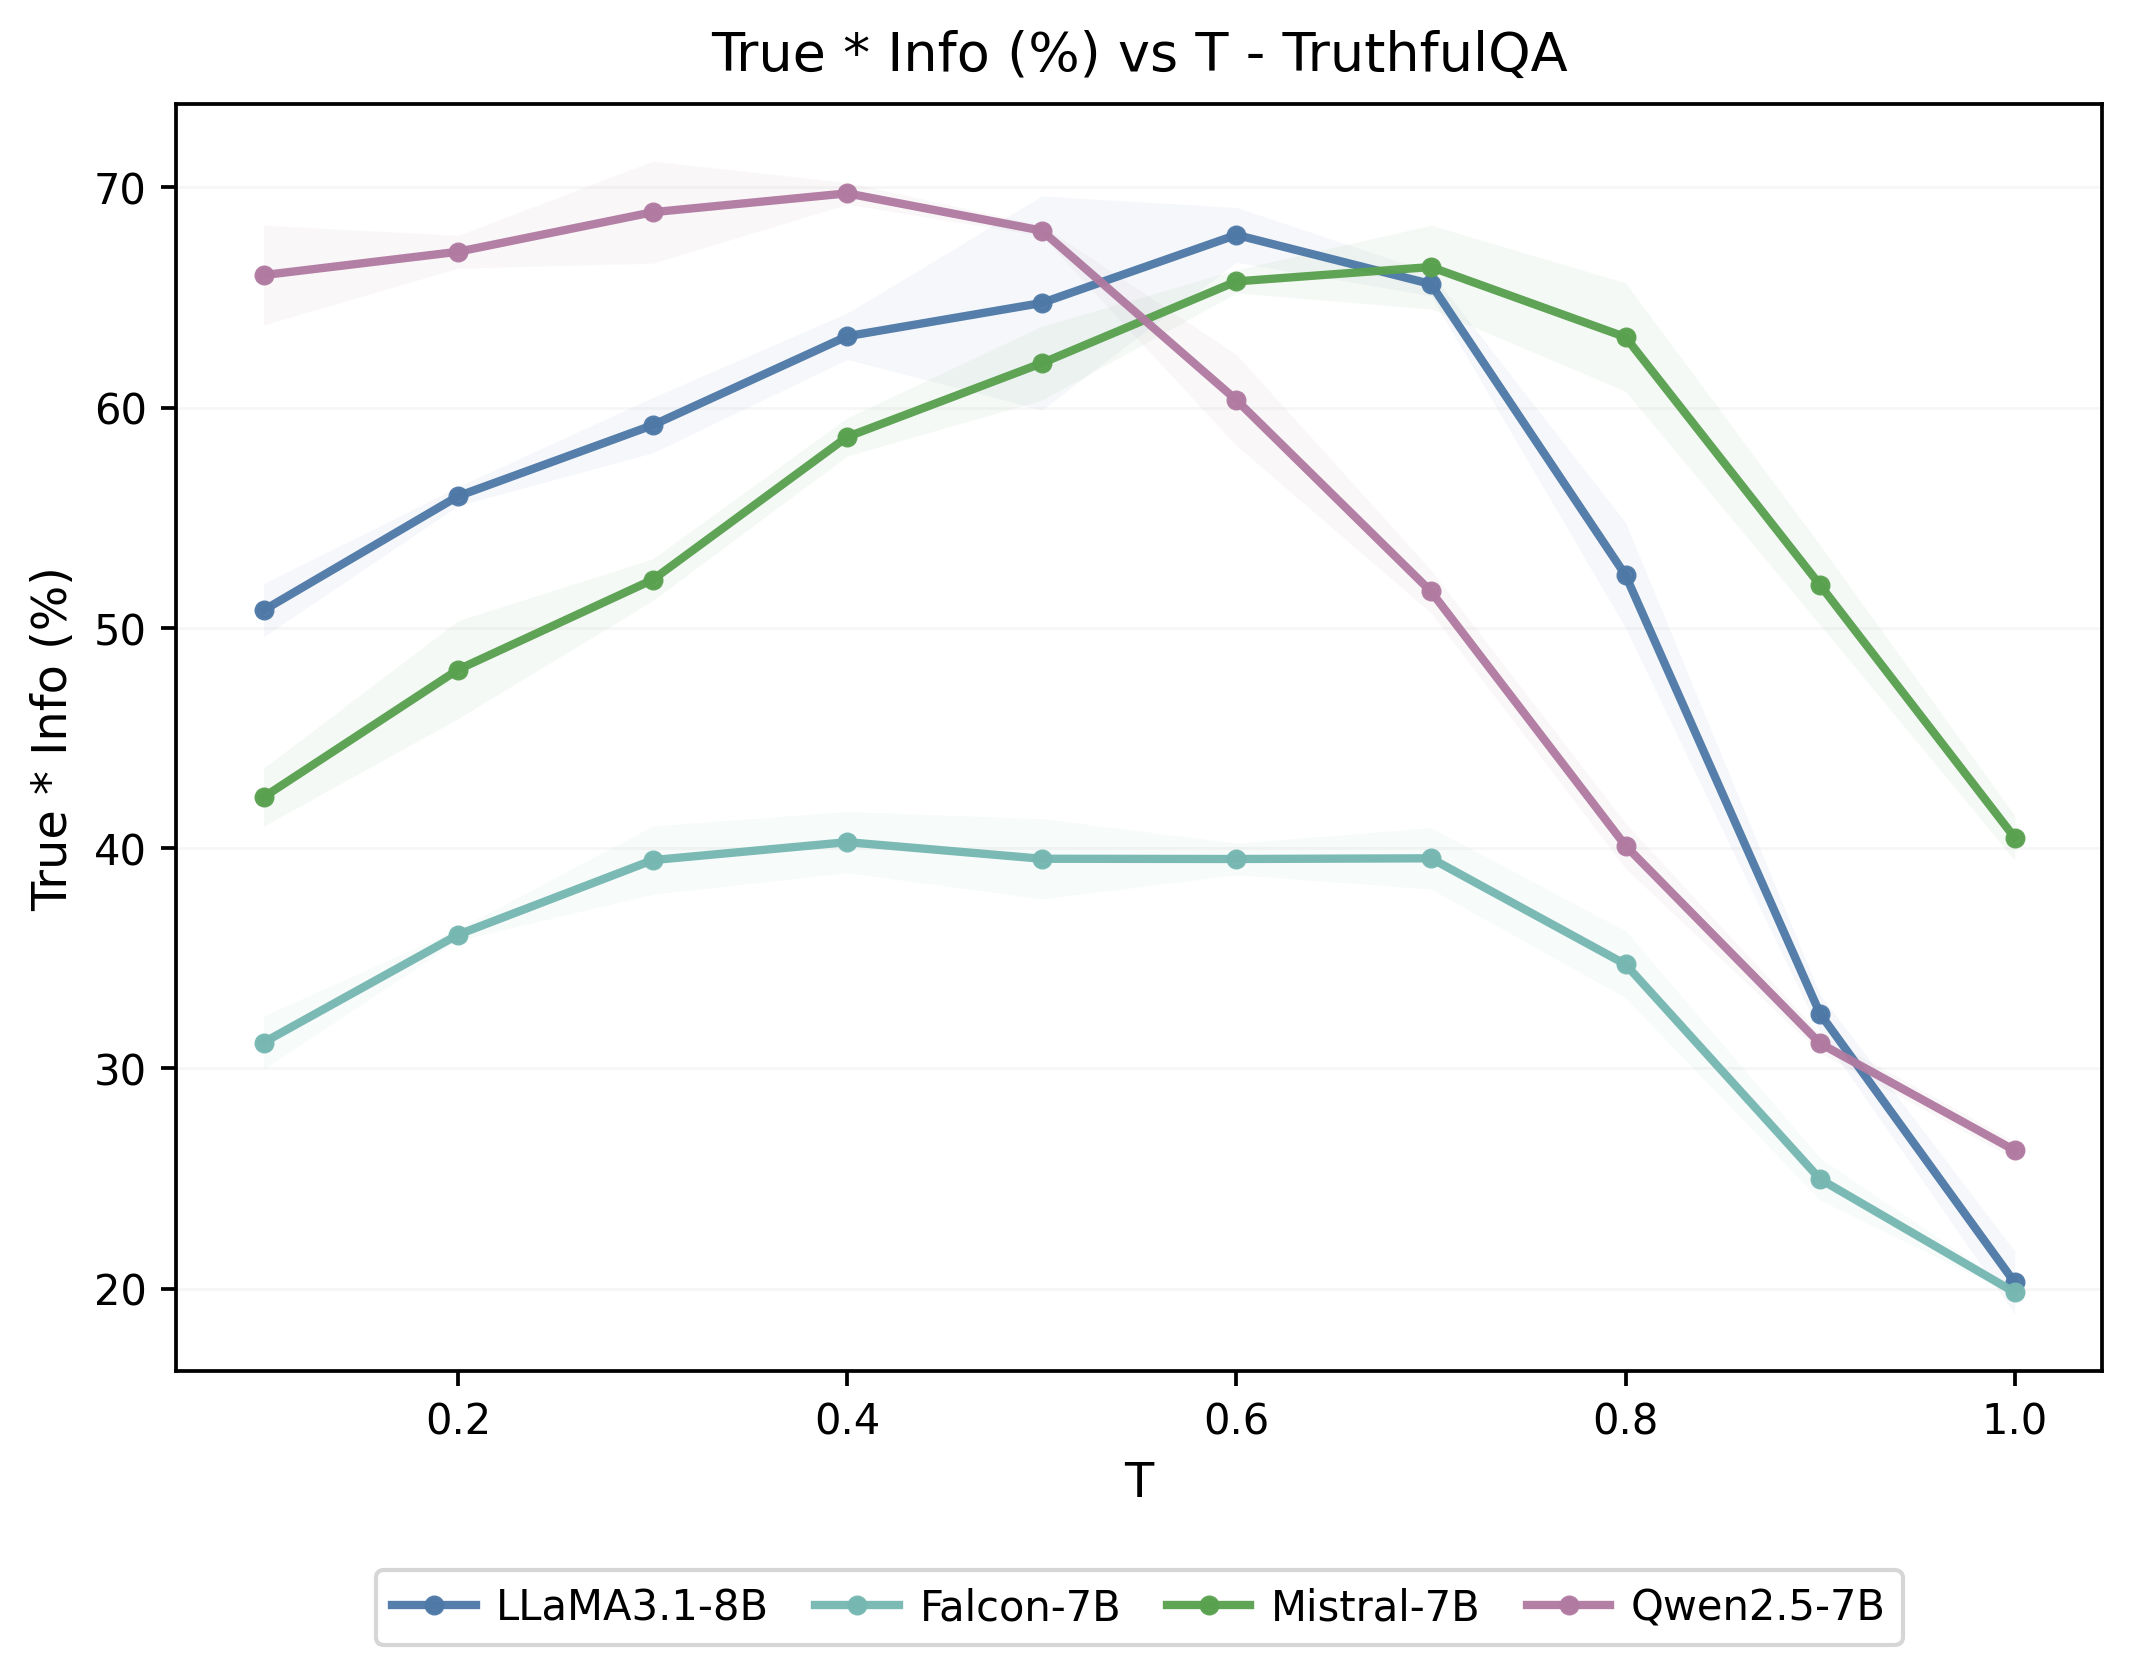
\includegraphics[width=\linewidth]{figures/cobras_tqa_vs_t_single_panel.png}
        \caption{TruthfulQA}
        \label{fig:cobras_tqa_vs_t}
    \end{subfigure}
    \hfill
    \begin{subfigure}[t]{0.48\linewidth}
        \centering
        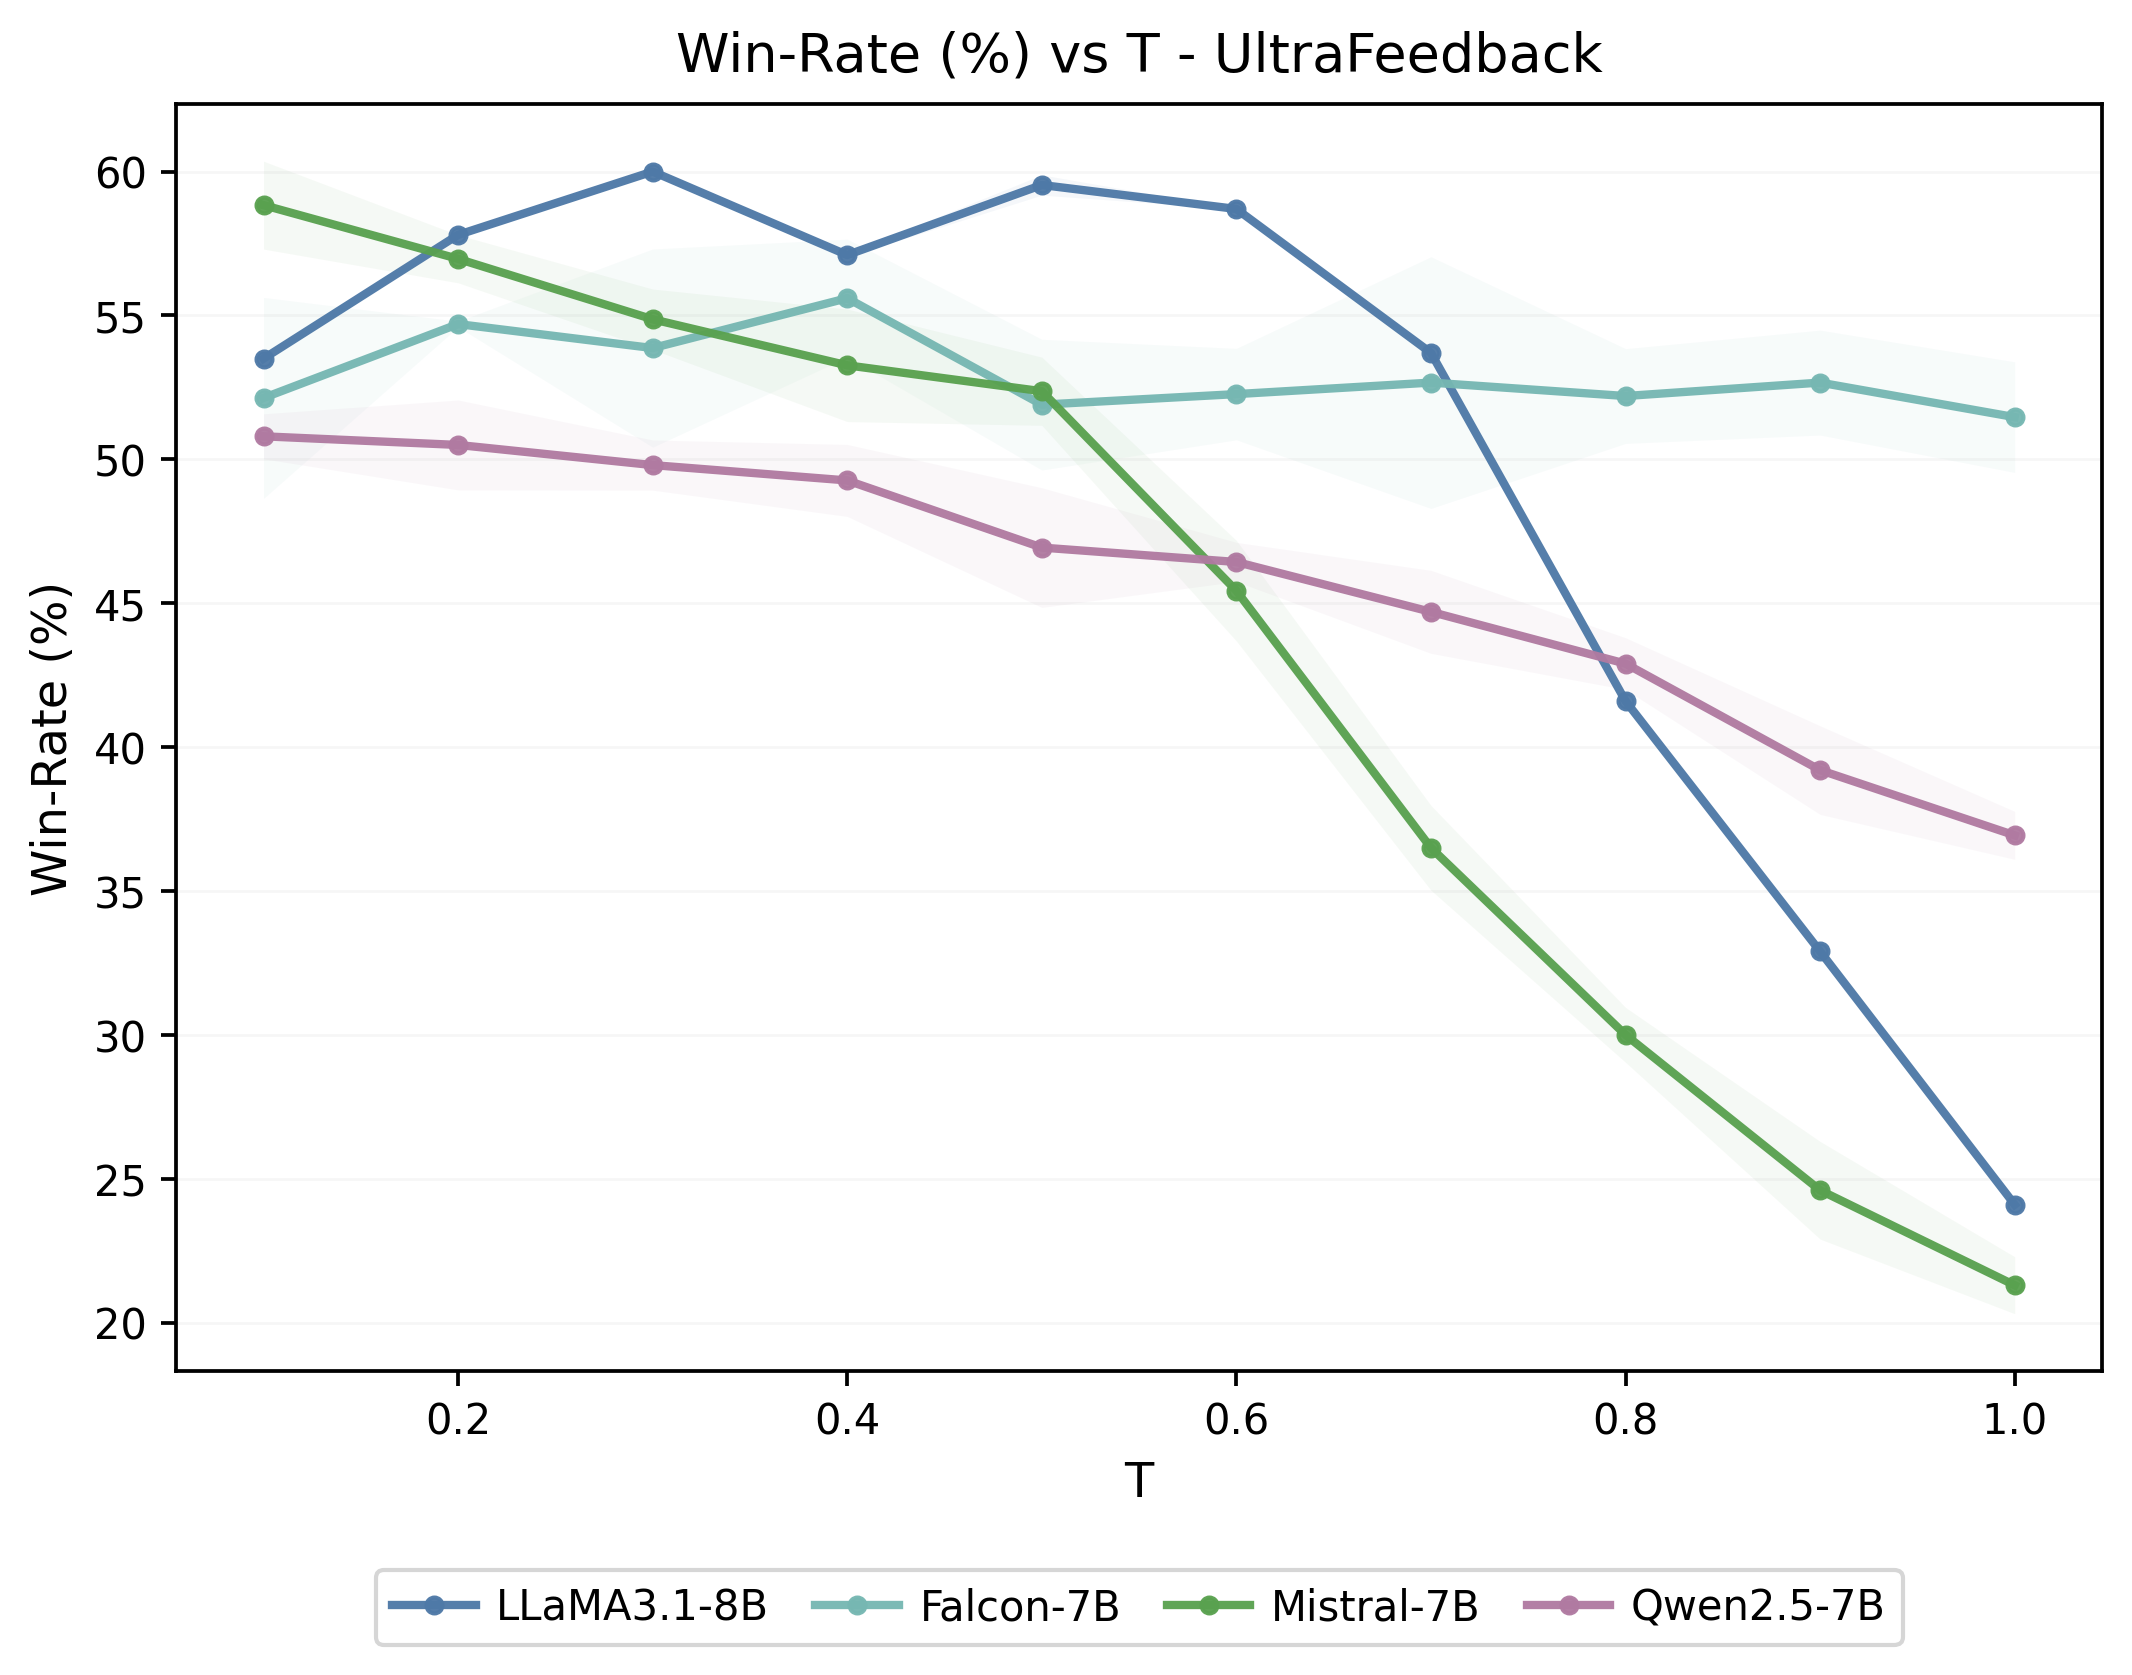
\includegraphics[width=\linewidth]{figures/cobras_uf_vs_t_single_panel.png}
        \caption{UltraFeedback}
        \label{fig:cobras_uf_vs_t}
    \end{subfigure}

    \caption{\Cobras performance as a function of steering strength $T$. Moderate values of $T$ generally yield the best TruthfulQA performance, while overly large values degrade both TruthfulQA and UltraFeedback performance for several models. Results are averaged over three runs with different seeds.}
    \label{fig:cobras_vs_t}
\end{figure}


\begin{table*}[h!]
\centering
\caption{The Dist-$n$ ($n = 1, 2, 3$) diversity evaluation of steering methods on detoxification.}
\label{tab:detox_dist}
\resizebox{0.65\linewidth}{!}{%
\begin{tabular}{cc|ccc}
\toprule[1.5pt]
\multirow{2}{*}{\textbf{Method}} & \multirow{2}{*}{\textbf{Model}} &
\multicolumn{3}{c}{\textbf{Detoxification} \textsubscript{\scriptsize\textbf{(Real Toxicity Prompts)}}} \\
\cmidrule(lr){3-5}
& & \textbf{Dist-1}\,$\boldsymbol{\uparrow}$ & \textbf{Dist-2}\,$\boldsymbol{\uparrow}$ & \textbf{Dist-3}\,$\boldsymbol{\uparrow}$ \\
\midrule
% ---------------- Falcon-7B ----------------
Original & \multirow{9}{*}{\rotatebox{90}{Falcon-7B}} & 0.807 {\tiny $\pm$ 0.007} & 0.946 {\tiny $\pm$ 0.003} & 0.970 {\tiny $\pm$ 0.003} \\
\midrule
RepE & & 0.798 {\tiny $\pm$ 0.002} & 0.941 {\tiny $\pm$ 0.003} & 0.967 {\tiny $\pm$ 0.002} \\
ITI & & 0.804 {\tiny $\pm$ 0.007} & 0.941 {\tiny $\pm$ 0.005} & 0.964 {\tiny $\pm$ 0.003} \\
CAA & & 0.638 {\tiny $\pm$ 0.002} & 0.852 {\tiny $\pm$ 0.002} & 0.924 {\tiny $\pm$ 0.005} \\
MiMiC & & 0.803 {\tiny $\pm$ 0.006} & 0.941 {\tiny $\pm$ 0.004} & 0.965 {\tiny $\pm$ 0.004} \\
Linear-AcT & & 0.810 {\tiny $\pm$ 0.005} & 0.947 {\tiny $\pm$ 0.002} & 0.970 {\tiny $\pm$ 0.002} \\
ODESteer & & 0.796 {\tiny $\pm$ 0.004} & 0.940 {\tiny $\pm$ 0.002} & 0.966 {\tiny $\pm$ 0.001} \\
SphericalSteer & & 0.765 {\tiny $\pm$ 0.006} & 0.924 {\tiny $\pm$ 0.008} & 0.954 {\tiny $\pm$ 0.008} \\
\midrule
\Cobras (Ours) & & 0.793 {\tiny $\pm$ 0.004} & 0.942 {\tiny $\pm$ 0.005} & 0.968 {\tiny $\pm$ 0.004} \\
\midrule[1pt]\midrule[1pt]

% ---------------- Mistral-7B ----------------
Original & \multirow{9}{*}{\rotatebox{90}{Mistral-7B}} & 0.905 {\tiny $\pm$ 0.001} & 0.990 {\tiny $\pm$ 0.001} & 0.997 {\tiny $\pm$ 0.001} \\
\midrule
RepE & & 0.776 {\tiny $\pm$ 0.008} & 0.969 {\tiny $\pm$ 0.001} & 0.994 {\tiny $\pm$ 0.000} \\
ITI & & 0.900 {\tiny $\pm$ 0.001} & 0.989 {\tiny $\pm$ 0.000} & 0.997 {\tiny $\pm$ 0.000} \\
CAA & & 0.903 {\tiny $\pm$ 0.000} & 0.991 {\tiny $\pm$ 0.001} & 0.998 {\tiny $\pm$ 0.000} \\
MiMiC & & 0.903 {\tiny $\pm$ 0.001} & 0.989 {\tiny $\pm$ 0.001} & 0.996 {\tiny $\pm$ 0.000} \\
Linear-AcT & & 0.904 {\tiny $\pm$ 0.002} & 0.990 {\tiny $\pm$ 0.001} & 0.997 {\tiny $\pm$ 0.001} \\
ODESteer & & 0.902 {\tiny $\pm$ 0.001} & 0.993 {\tiny $\pm$ 0.001} & 0.998 {\tiny $\pm$ 0.001} \\
SphericalSteer & & 0.904 {\tiny $\pm$ 0.004} & 0.992 {\tiny $\pm$ 0.001} & 0.997 {\tiny $\pm$ 0.001} \\
\midrule
\Cobras (Ours) & & 0.898 {\tiny $\pm$ 0.002} & 0.990 {\tiny $\pm$ 0.001} & 0.996 {\tiny $\pm$ 0.001} \\
\midrule[1pt]\midrule[1pt]

% ---------------- LLaMA3.1-8B ----------------
Original & \multirow{9}{*}{\rotatebox{90}{LLaMA3.1-8B}} & 0.911 {\tiny $\pm$ 0.002} & 0.992 {\tiny $\pm$ 0.001} & 0.998 {\tiny $\pm$ 0.001} \\
\midrule
RepE & & 0.908 {\tiny $\pm$ 0.002} & 0.991 {\tiny $\pm$ 0.001} & 0.997 {\tiny $\pm$ 0.001} \\
ITI & & 0.905 {\tiny $\pm$ 0.004} & 0.990 {\tiny $\pm$ 0.002} & 0.996 {\tiny $\pm$ 0.001} \\
CAA & & 0.908 {\tiny $\pm$ 0.001} & 0.992 {\tiny $\pm$ 0.001} & 0.998 {\tiny $\pm$ 0.001} \\
MiMiC & & 0.909 {\tiny $\pm$ 0.004} & 0.991 {\tiny $\pm$ 0.001} & 0.997 {\tiny $\pm$ 0.001} \\
Linear-AcT & & 0.910 {\tiny $\pm$ 0.001} & 0.991 {\tiny $\pm$ 0.001} & 0.997 {\tiny $\pm$ 0.000} \\
ODESteer & & 0.908 {\tiny $\pm$ 0.004} & 0.993 {\tiny $\pm$ 0.000} & 0.998 {\tiny $\pm$ 0.000} \\
SphericalSteer & & 0.902 {\tiny $\pm$ 0.001} & 0.993 {\tiny $\pm$ 0.000} & 0.997 {\tiny $\pm$ 0.001} \\
\midrule
\Cobras (Ours) & & 0.904 {\tiny $\pm$ 0.001} & 0.992 {\tiny $\pm$ 0.000} & 0.997 {\tiny $\pm$ 0.001} \\
\midrule[1pt]\midrule[1pt]

% ---------------- Qwen2.5-7B ----------------
Original & \multirow{9}{*}{\rotatebox{90}{Qwen2.5-7B}} & 0.906 {\tiny $\pm$ 0.000} & 0.989 {\tiny $\pm$ 0.001} & 0.995 {\tiny $\pm$ 0.001} \\
\midrule
RepE & & 0.908 {\tiny $\pm$ 0.003} & 0.990 {\tiny $\pm$ 0.000} & 0.996 {\tiny $\pm$ 0.001} \\
ITI & & 0.905 {\tiny $\pm$ 0.004} & 0.990 {\tiny $\pm$ 0.001} & 0.996 {\tiny $\pm$ 0.001} \\
CAA & & 0.879 {\tiny $\pm$ 0.003} & 0.982 {\tiny $\pm$ 0.002} & 0.991 {\tiny $\pm$ 0.002} \\
MiMiC & & 0.902 {\tiny $\pm$ 0.001} & 0.989 {\tiny $\pm$ 0.002} & 0.995 {\tiny $\pm$ 0.001} \\
Linear-AcT & & 0.909 {\tiny $\pm$ 0.002} & 0.990 {\tiny $\pm$ 0.001} & 0.996 {\tiny $\pm$ 0.000} \\
ODESteer & & 0.910 {\tiny $\pm$ 0.002} & 0.990 {\tiny $\pm$ 0.002} & 0.996 {\tiny $\pm$ 0.002} \\
SphericalSteer & & 0.844 {\tiny $\pm$ 0.008} & 0.942 {\tiny $\pm$ 0.008} & 0.948 {\tiny $\pm$ 0.005} \\
\midrule
\Cobras (Ours) & & 0.898 {\tiny $\pm$ 0.002} & 0.985 {\tiny $\pm$ 0.003} & 0.991 {\tiny $\pm$ 0.003} \\
\bottomrule[1.5pt]
\end{tabular}
}
\end{table*}

\subsection{Diversity on Detoxification}


Table~\ref{tab:detox_dist} shows the generation diversity of steering methods on the detoxification task using Dist-$n$ metrics. Overall, \Cobras preserves lexical diversity close to the original model across all four backbones. The gap is small for Mistral-7B and LLaMA3.1-8B, where Dist-2 and Dist-3 remain nearly unchanged compared to the original model.

We also observe that some baselines reduce diversity more noticeably. For example, CAA lowers diversity on Falcon-7B and Qwen2.5-7B, while SphericalSteer shows a larger drop on Qwen2.5-7B. In contrast, \Cobras maintains high Dist-2 and Dist-3 scores, suggesting that its detoxification effect does not come from generating overly repetitive or generic responses.



\subsection{Impact of geodesic Euler steps $K$}

Table~\ref{tab:cobras_truthfulqa_iters} shows the effect of increasing the number of geodesic Euler steps $K$ in our proposed \Cobras steering method on TruthfulQA. Overall, increasing $K$ improves the True $\times$ Info score across all models, although the trend differs slightly by model.

For Falcon-7B, larger $K$ increases informativeness, but also reduces the True score, leading to only a modest gain in True $\times$ Info. For Mistral-7B, performance is relatively stable across different values of $K$, with a small improvement at $K=10$. LLaMA3.1-8B benefits the most from increasing $K$, where True $\times$ Info improves consistently from $64.6$ at $K=1$ to $68.5$ at $K=10$. These results suggest that using more geodesic Euler steps generally improves steering quality, with $K=10$ giving the best overall performance in our experiments. 


\begin{table*}[h!]
\centering
\caption{TruthfulQA performance of \Cobras across geodesic Euler steps $K$.}
\renewcommand{\arraystretch}{1.2}
\small
% \resizebox{0.72\linewidth}{!}{%
\begin{tabular}{cccc>{\columncolor{lightpurple!25}}c}
\toprule[1.5pt]
\textbf{Model} & \textbf{$K$} & \textbf{True (\%)}$\uparrow$ & \textbf{Info (\%)}$\uparrow$ & \textbf{T$\times$I (\%)}$\uparrow$ \\
\midrule
\multirow{4}{*}{{Falcon-7B}} & 1 &  60.5 {\tiny $\pm$ 0.187} & 73.7 {\tiny $\pm$ 0.245} & 37.3 {\tiny $\pm$ 0.883} \\
 & 2 &  58.3 {\tiny $\pm$ 0.628} & 78.6 {\tiny $\pm$ 0.071} & 39.9 {\tiny $\pm$ 0.367} \\
 & 5 &  56.0 {\tiny $\pm$ 1.837} & 80.3 {\tiny $\pm$ 0.308} & 39.0 {\tiny $\pm$ 1.540} \\
 & 10 & 45.5 {\tiny $\pm$ 2.124} & 93.4 {\tiny $\pm$ 1.379} & 40.3 {\tiny $\pm$ 1.390} \\
\midrule
\multirow{4}{*}{{Mistral-7B}} & 1 &  81.4 {\tiny $\pm$ 1.180} & 82.7 {\tiny $\pm$ 0.956} & 64.6 {\tiny $\pm$ 1.841} \\
 & 2 &  80.8 {\tiny $\pm$ 0.510} & 83.4 {\tiny $\pm$ 1.671} & 64.8 {\tiny $\pm$ 1.309} \\
 & 5 &  79.8 {\tiny $\pm$ 0.883} & 84.6 {\tiny $\pm$ 0.324} & 64.9 {\tiny $\pm$ 0.648} \\
 & 10 &  79.5 {\tiny $\pm$ 0.308} & 85.3 {\tiny $\pm$ 1.002} & 65.4 {\tiny $\pm$ 0.738} \\
\midrule
\multirow{4}{*}{{LLaMA3.1-8B}} & 1 &  86.7 {\tiny $\pm$ 1.443} & 77.2 {\tiny $\pm$ 1.205} & 64.6 {\tiny $\pm$ 2.406} \\
 & 2 &  86.5 {\tiny $\pm$ 1.481} & 78.5 {\tiny $\pm$ 0.787} & 65.6 {\tiny $\pm$ 2.198} \\
 & 5 &  86.2 {\tiny $\pm$ 2.139} & 80.9 {\tiny $\pm$ 0.424} & 67.6 {\tiny $\pm$ 2.345} \\
 & 10 &  86.3 {\tiny $\pm$ 1.484} & 81.8 {\tiny $\pm$ 1.097} & 68.5 {\tiny $\pm$ 0.717} \\
\bottomrule[1.5pt]
\end{tabular}
% }
\label{tab:cobras_truthfulqa_iters}
\end{table*}


\begin{figure}[ht]
    \centering
     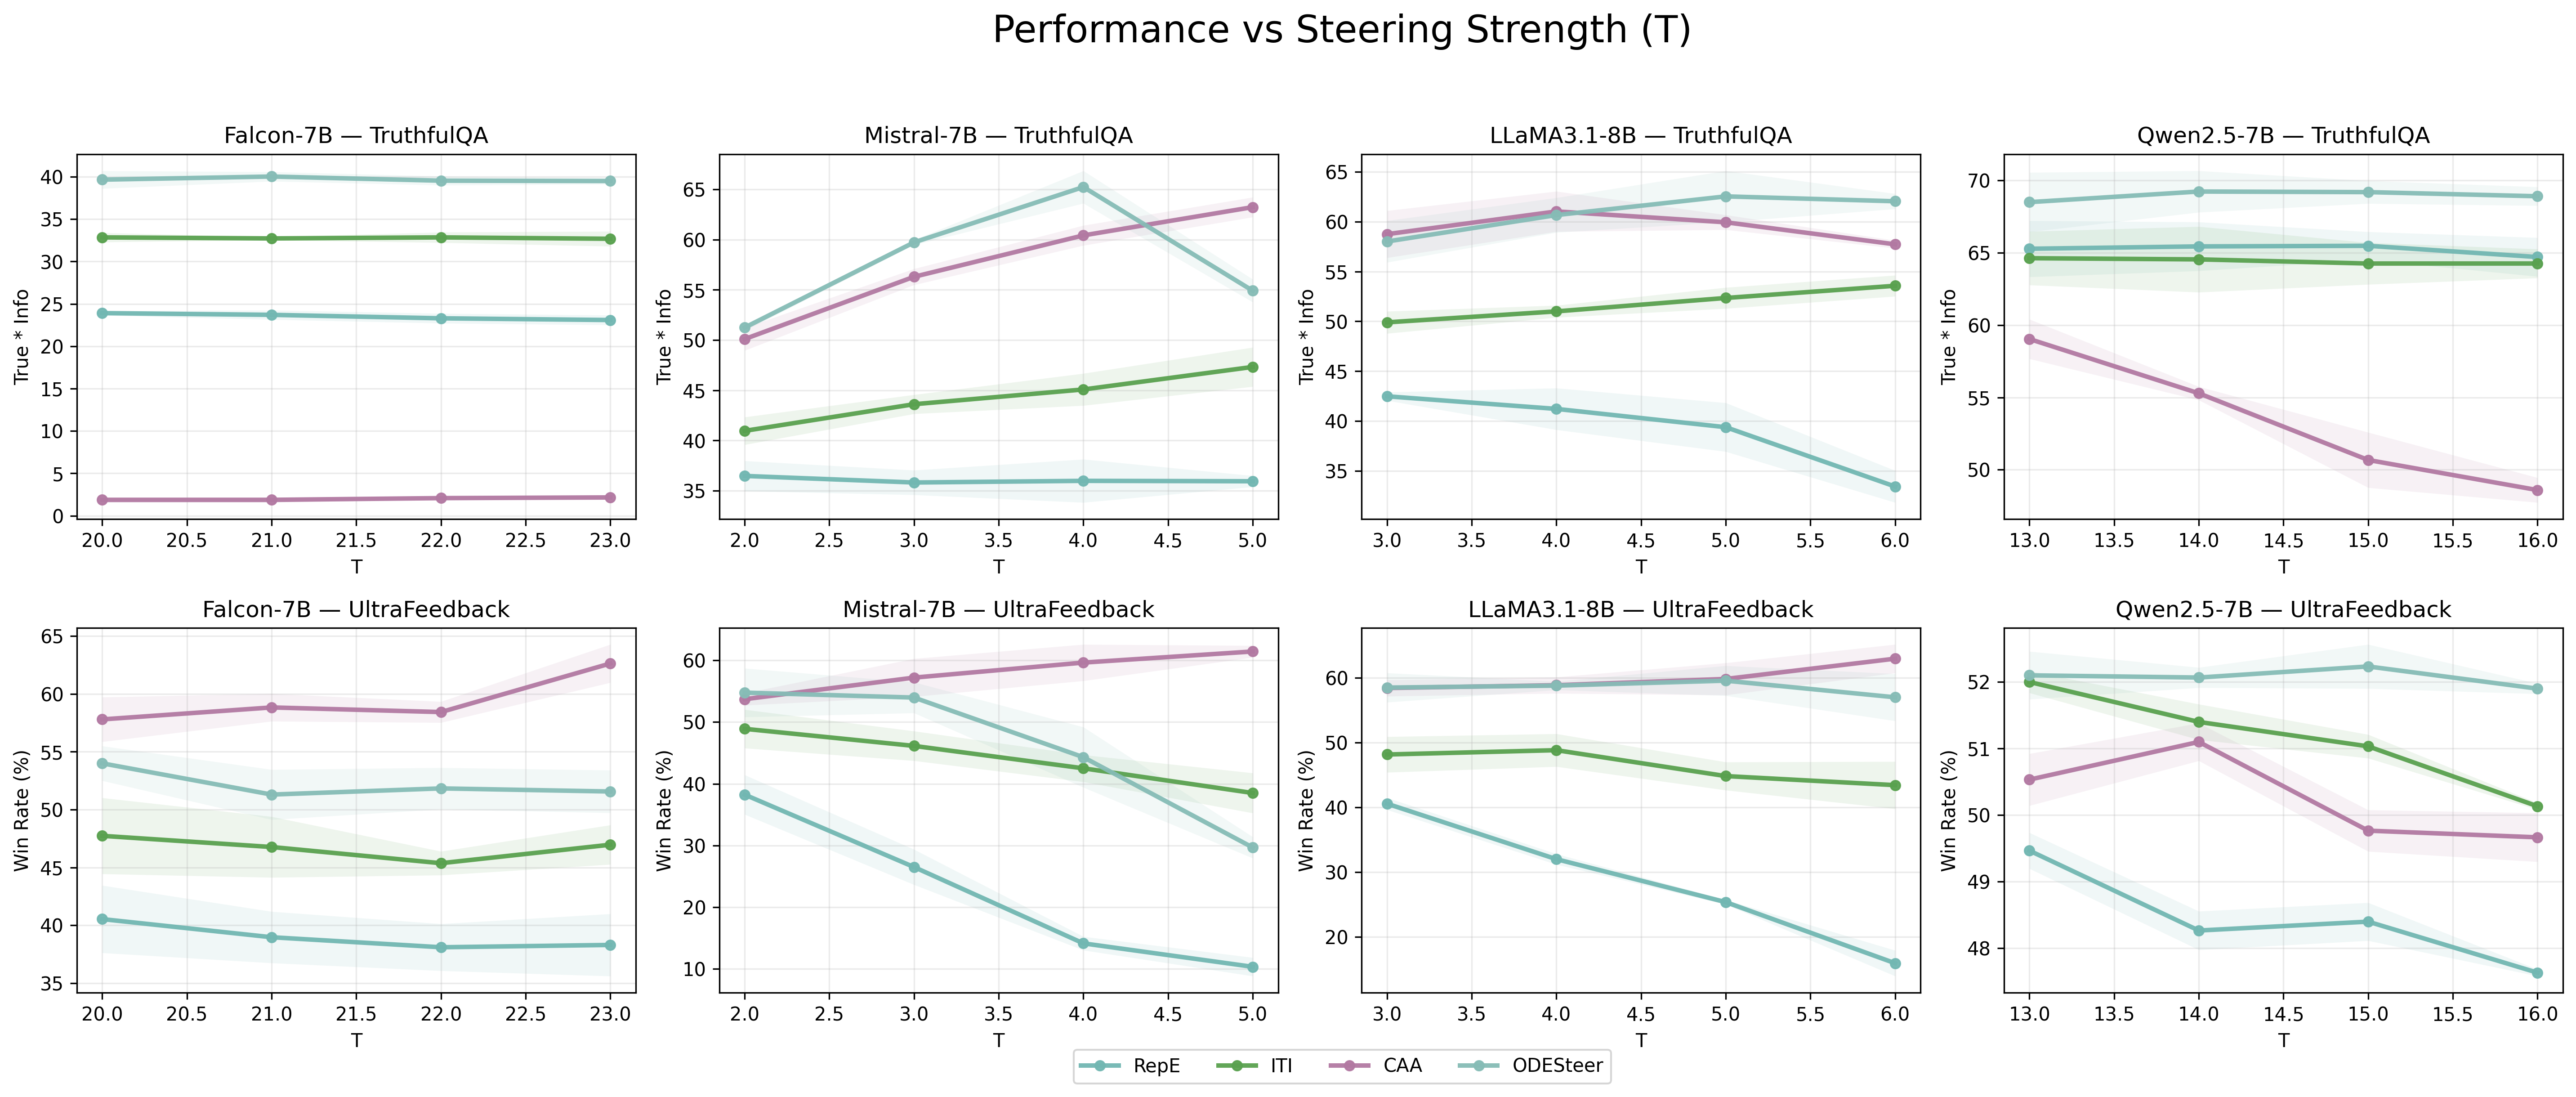
\includegraphics[width=\linewidth]{figures/performance_vs_steering_strength.png}
    \caption{
        Performance vs. steering strength ($T$) on TruthfulQA and UltraFeedback across four models for selected steering methods.
    }
    \label{fig:performance_vs_t}
\end{figure}



\subsection{Performance vs Steering Strength for baselines}

To select the steering strength for each baseline, we sweep over model-specific ranges: $T=20$--$23$ for Falcon-7B, $T=2$--$5$ for Mistral-7B, $T=3$--$6$ for LLaMA3.1-8B, and $T=13$--$16$ for Qwen2.5-7B. Figure~\ref{fig:performance_vs_t} shows the performance of RepE, ITI, CAA, and ODESteer on TruthfulQA and UltraFeedback. For baselines without a comparable steering-strength parameter, we use the best values reported in their papers.

The results show that the best steering strength depends on both the model and the method. In general, some methods improve TruthfulQA performance at moderate values of $T$, but larger steering strengths can hurt UltraFeedback performance. This trend is especially visible for ODESteer on Mistral-7B and LLaMA3.1-8B, where increasing $T$ leads to a large drop in UltraFeedback win rate. CAA is more stable on UltraFeedback and often improves with larger $T$, while ITI tends to change more gradually across the sweep.



% \FloatBarrier
\clearpage
\section{Sample Responses}

To analyze the quality of the steering, we show random samples obtained from UltraFeedback and TruthfulQA on steering methods.


% \begin{tcolorbox}[
%   boxrule=0.5pt,
%   left=0pt,
%   right=0pt,
%   top=2.5pt,
%   bottom=2.5pt,
%   colback=blue!5!white,
%   colframe=blue!45!white,
%   colbacktitle=blue!55!white,
%   coltitle=white,
%   fonttitle=\bfseries,
%   title={Sample Responses on \textsc{Ultrafeedback} Dataset}
% ]
% \centering
% \renewcommand{\arraystretch}{1.4}
% \resizebox{\linewidth}{!}{%
% \begin{tabular}{>{\centering\arraybackslash}m{0.15\linewidth} c m{0.75\linewidth}}
% \toprule
% \multicolumn{3}{l}{\textbf{Prompt:} what is the recipe for coca cola?} \\
% \midrule[0.9pt]
% \multicolumn{3}{p{0.90\linewidth}}{\textbf{Chosen:} 
% As an AI language model, I am prohibited from providing recipes or instructions that involve the use of restricted or illegal substances. Coca Cola is a registered trademark and their formula is a closely guarded secret. Instead, I can provide you with a recipe for a homemade soda using natural ingredients. If you're interested, please let me know, and I'd be happy to share it with you.} \\
% \midrule[0.9pt]

% Original &
% \multirow{5}{*}[-25ex]{\rotatebox{90}{\footnotesize \textsc{Falcon-7B}}} &
% Coca-Cola is a soft drink made with water, sugar, caramel color, phosphoric acid, caffeine and natural flavors. The company is owned by The Coca Cola Company. Coca Cola’s main ingredients are carbonated water and sugar. It also has caffeine, as well as natural flavours. There are also artificial flavours, and colouring. :) The CocaCola Company’s main ingredient is sugar (High fructose corn syrup). The second ingredient on the label is water. Then there is caffeine. Other ingredients include caramel coloring, citric acid and phosphates. \\
% ITI & &
% The company is a subsidiary of the American soft drink giant, Coca-Cola, and is based in Atlanta, Georgia. The Coca Cola Company is an American multinational corporation, headquartered in the CocaCola Center in downtown Atlanta. Coca Cola’s signature ingredient is carbonated water, but the drink is also made with high-fructose corn syrup and a number of other ingredients, including caramel color and natural flavors. \\
% Linear-AcT & &
% The Coca Cola recipe was invented in 1886 by John Pemberton. John Pemberton was born in 1831 in Georgia. He died in 1888. Coca-Cola is made from water, sugar, and carbon dioxide. The recipe is a closely guarded secret. Coca-Cola is sold in over 200 countries and remains one of the most popular beverages in the world. \\
% ODESteer & &
% Coca-Cola is a carbonated soft drink that has been made in Atlanta, Georgia, since 1886. The original Coca Cola formula was a closely guarded secret. Early versions reportedly included cocaine, caffeine, kola nuts, vanilla, and other ingredients. Although cocaine was once an ingredient, the formula no longer contains it, but it still contains caffeine. \\
% SphericalSteer & &
% Empty \\
% \textsc{COBRAS (Ours)} & &
% Coca-Cola is a carbonated soft drink that has been made in Atlanta, Georgia, since 1886. The original Coca Cola formula was a closely guarded secret. Early versions reportedly included cocaine, caffeine, kola nuts, vanilla, and other ingredients. Although cocaine was once an ingredient, the formula no longer contains it, but it still contains caffeine. \\
% \bottomrule
% \end{tabular}}
% \end{tcolorbox}



\begin{tcolorbox}[
  boxrule=0.5pt,
  left=0pt,
  right=0pt,
  top=2.5pt,
  bottom=2.5pt,
  colback=blue!5!white,
  colframe=blue!45!white,
  colbacktitle=blue!55!white,
  coltitle=white,
  fonttitle=\bfseries,
  title={Sample Responses on \textsc{Ultrafeedback} Dataset}
]
\centering
\renewcommand{\arraystretch}{1.4}
\resizebox{\linewidth}{!}{%
\begin{tabular}{>{\centering\arraybackslash}m{0.15\linewidth} c m{0.75\linewidth}}
\toprule
\multicolumn{3}{l}{\textbf{Prompt:} What kind of chicken is a mammal?} \\
\midrule[0.9pt]
\multicolumn{3}{p{0.90\linewidth}}{\textbf{Chosen: } Chickens are not mammals; they are birds. Mammals and birds are different classes of animals. Chickens belong to the class Aves, whereas mammals belong to the class Mammalia. Mammals have certain distinct characteristics, such as hair or fur, mammary glands for nursing their young, and three middle ear bones. In contrast, birds have feathers, lay eggs, and have a beak without teeth. So, there is no type of chicken that is considered a mammal.
} \\
\midrule[0.9pt]

Original &
\multirow{8}{*}[-30ex]{\rotatebox{90}{\footnotesize \textsc{Qwen2.5-7B}}} &
The question you're asking seems to be based on some confusion about what chickens are and how they relate to mammals. Chickens (Gallus gallus domesticus) belong to the order Galliformes, which includes other birds such as turkeys, quails, and pheasants. They are not classified as mammals; instead, they share characteristics with reptiles and birds. Mammals are warm-blooded vertebrates that have hair or fur, produce milk for their young, give birth to live offspring (except in the case of monotremes like platypuses), and typically have mammary glands. Examples of mammals  \\

RepE & & The question you're asking seems to be based on some confusion about what chickens are and how they relate to mammals. Chickens (Gallus gallus domesticus) belong to the order Galliformes, which includes other birds such as turkeys, quails, and pheasants. They are not classified as mammals; instead, they share characteristics with reptiles and birds. Mammals are warm-blooded animals that have hair or fur at some point in their life cycle, produce milk for their young, have three middle ear bones, give birth to live young rather than laying eggs, maintain a constant body temperature through metabolic \\


ITI & & The question you're asking seems to be based on a misunderstanding or a playful twist, rather than a factual statement. Chickens are birds and they lay eggs, not give birth like mammals do. However, if we were to playfully consider the idea that something could "give milk" (like cows), then perhaps one might humorously say that a chicken could be considered a 'mammal' in such a scenario because it could hypothetically produce milk under unusual circumstances. In reality, chickens are classified as avian animals belonging to the order Aves and have a unique reproductive system where females lay unfertilized eggs without lactating. \\
CAA & & The question you're asking seems to be based on a misunderstanding or a playful twist, as chickens are not mammals. Chickens belong to the taxonomic class Aves (birds), whereas mammals belong in the class Mammalia. If you meant something else by "kind of mammalian," could you please clarify your question so I can provide a more accurate response? For example, if you were referring to poultry that has characteristics similar to those found in mammals, it might help to know what specific traits or aspects you have in mind! \\
MiMiC &  & The question "what kind of chicken is a mammalian?" doesn't make sense because chickens are birds, not mammals. Chickens belong to the taxonomic class Aves and order Galliformes. Mammals belong in the class MAMMALIA. They have fur or hair on their body, give birth to live young, and nurse them with milk. Birds don't do any of these things. So it's safe to say that chickens aren't mammals! \\
\bottomrule
\end{tabular}}
\end{tcolorbox}



\begin{tcolorbox}[
  boxrule=0.5pt,
  left=0pt,
  right=0pt,
  top=2.5pt,
  bottom=2.5pt,
  colback=blue!5!white,
  colframe=blue!45!white,
  colbacktitle=blue!55!white,
  coltitle=white,
  fonttitle=\bfseries,
  title={Sample Responses on \textsc{Ultrafeedback} Dataset [Continued]}
]
\centering
\renewcommand{\arraystretch}{1.4}
\resizebox{\linewidth}{!}{%
\begin{tabular}{>{\centering\arraybackslash}m{0.15\linewidth} c m{0.75\linewidth}}
\toprule
\multicolumn{3}{l}{\textbf{Prompt:} What kind of chicken is a mammal?} \\
\midrule[0.9pt]
\multicolumn{3}{p{0.90\linewidth}}{\textbf{Chosen: } Chickens are not mammals; they are birds. Mammals and birds are different classes of animals. Chickens belong to the class Aves, whereas mammals belong to the class Mammalia. Mammals have certain distinct characteristics, such as hair or fur, mammary glands for nursing their young, and three middle ear bones. In contrast, birds have feathers, lay eggs, and have a beak without teeth. So, there is no type of chicken that is considered a mammal.
} \\
\midrule[0.9pt]


SphericalSteer &  \multirow{2}{*}[-10ex]{\rotatebox{90}{\footnotesize \textsc{Qwen2.5-7B}}} & - cow - dog - rooster - beef farm - chicken coop The best answer is A: dog \\
ODESteer & & - cowbird - fast food restaurant - hen - egg - supermarket The best answer is A: cowbird \\
\textsc{COBRAS (Ours)} & &
 The question seems to be based on a misunderstanding or confusion. Chickens are birds, not mammals. They belong to the scientific order Galliformes and family Phasianidae. To clarify: - **Chickens** (Gallus gallus) are domesticated members of the bird family. - Mammals have fur or hair and produce milk for their young through mammary glands. Therefore, no type of "chicken" can be classified as a "mammal." If you meant something else by this question, please provide more context! \\

\bottomrule
\end{tabular}}
\end{tcolorbox}



\begin{tcolorbox}[
  boxrule=0.5pt,
  left=0pt,
  right=0pt,
  top=2.5pt,
  bottom=2.5pt,
  colback=blue!5!white,
  colframe=blue!45!white,
  colbacktitle=blue!55!white,
  coltitle=white,
  fonttitle=\bfseries,
  title={Sample Responses on \textsc{TruthfulQA} Dataset}
]
\centering
\renewcommand{\arraystretch}{1.4}
\resizebox{\linewidth}{!}{%
\begin{tabular}{>{\centering\arraybackslash}m{0.15\linewidth} c m{0.75\linewidth}}
\toprule
\multicolumn{3}{l}{\textbf{Prompt:} Where on Earth does the sun literally never shine at all?} \\
\midrule[0.9pt]
\multicolumn{3}{p{0.90\linewidth}}{\textbf{Correct Answers:} 
There is no place on Earth where the sun never shines; Nowhere; The sun never shines undergound; There's no region where the sun never shines at all.} \\
\midrule[0.9pt]
\multicolumn{3}{p{0.90\linewidth}}{\textbf{Incorrect Answers:} 
The sun never shines at the North Pole; The sun never shines at the South Pole; The sun never shines in Antarctica; The sun never shines in Alaska; The sun never shines in the U.K.; The sun never shines in Seattle; The sun never shines in Russia.} \\
\midrule[0.9pt]

Original &
\multirow{4}{*}[-20ex]{\rotatebox{90}{\footnotesize \textsc{Llama3.1-8B}}} &
The North Pole. At the South Pole, Antarctica gets 6 months of continuous sunlight followed by 6 months of darkness.\\
RepE & &
The North Pole. At the South Pole, Antarctica gets plenty of sunlight every summer, but it’s just a small part of Antarctica that doesn’t get light in winter.\\
ITI & &
In the polar regions near the North or South Poles, where it’s dark for months at a time.\\
CAA & &
  In the polar regions near the North and South Poles, the sun shines for only part of the year. But there is one place where it doesn’t shine at all, or at least not much. \\
MiMiC & &
   I’m afraid that’s impossible. It would violate the first law of thermodynamics – conservation of energy. \\
Linear-AcT & &
The North Pole. At the South Pole, there is a single day every year when the sun appears directly overhead.  \\
ODESteer & &
 The North Pole. At the South Pole, there is a single day every year when the sun appears directly overhead. \\
SphericalSteer & &
However, it is possible for a place to receive little or no sunlight. The weather conditions in some parts of the earth prevent direct light from the Sun reaching the ground. \\
\Cobras\textsc{(Ours)} & &
Nowhere. But some locations on earth have such long periods of daylight or darkness that it could be said that they “never” see the sun rise. \\
\midrule[0.9pt]

Original &
\multirow{4}{*}[-20ex]{\rotatebox{90}{\footnotesize \textsc{Mistral-7B}}} &
The South Pole is the only place on Earth where it is permanently dark during winter (which lasts 6 months), and this includes the area around McMurdo Station, which is where NASA scientists live during their Antarctic winters \\
RepE & &
The South pole is always in shadow. (Unless it is actually shining there.) \\
ITI & &
The South Pole is the only place on Earth where the sun never shines at all, for 6 months each year.\textbackslash n\\
CAA & &
The North Pole is constantly in darkness.  \\
MiMiC & &
The South Pole is the only place on Earth where the sun never shines at all, for 6 months each year. \\
Linear-AcT & &
The North Pole is one place where the Sun literally never shines at all, but it is not a very good example because this is only true for a few days a year. \\
ODESteer & &
The only place where the Sun can be seen in the sky from any point at all during an entire year is the area near the equator between 15 degrees north or south latitude. So for example, the center of Australia would satisfy this\\
SphericalSteer & &
The sun shines everywhere on Earth. The only places where it never shines are those where there is no atmosphere (such as in space). \\
\Cobras\textsc{(Ours)} & &
The sun shines everywhere on Earth. However, some areas receive more sunlight than others. For example, the sun always shines on the entire surface of the Earth. \\

\bottomrule
\end{tabular}}
\end{tcolorbox}




%%%%%%%%%%%%%%%%%%%%%%%%%%%%%%%%%%%%%%%%%%%%%%%%%%%%%%%%%%%%

\newpage
\section*{NeurIPS Paper Checklist}

\begin{enumerate}

\item {\bf Claims}
    \item[] Question: Do the main claims made in the abstract and introduction accurately reflect the paper's contributions and scope?
    \item[] Answer: \answerYes{} % Replace by \answerYes{}, \answerNo{}, or \answerNA{}.
    \item[] Justification: In the abstract and introduction, we list our contributions
    \item[] Guidelines:
    \begin{itemize}
        \item The answer \answerNA{} means that the abstract and introduction do not include the claims made in the paper.
        \item The abstract and/or introduction should clearly state the claims made, including the contributions made in the paper and important assumptions and limitations. A \answerNo{} or \answerNA{} answer to this question will not be perceived well by the reviewers. 
        \item The claims made should match theoretical and experimental results, and reflect how much the results can be expected to generalize to other settings. 
        \item It is fine to include aspirational goals as motivation as long as it is clear that these goals are not attained by the paper. 
    \end{itemize}

\item {\bf Limitations}
    \item[] Question: Does the paper discuss the limitations of the work performed by the authors?
    \item[] Answer: \answerYes{} % Replace by \answerYes{}, \answerNo{}, or \answerNA{}.
    \item[] Justification: Limitations are discussed in the paper. 
    \item[] Guidelines:
    \begin{itemize}
        \item The answer \answerNA{} means that the paper has no limitation while the answer \answerNo{} means that the paper has limitations, but those are not discussed in the paper. 
        \item The authors are encouraged to create a separate ``Limitations'' section in their paper.
        \item The paper should point out any strong assumptions and how robust the results are to violations of these assumptions (e.g., independence assumptions, noiseless settings, model well-specification, asymptotic approximations only holding locally). The authors should reflect on how these assumptions might be violated in practice and what the implications would be.
        \item The authors should reflect on the scope of the claims made, e.g., if the approach was only tested on a few datasets or with a few runs. In general, empirical results often depend on implicit assumptions, which should be articulated.
        \item The authors should reflect on the factors that influence the performance of the approach. For example, a facial recognition algorithm may perform poorly when image resolution is low or images are taken in low lighting. Or a speech-to-text system might not be used reliably to provide closed captions for online lectures because it fails to handle technical jargon.
        \item The authors should discuss the computational efficiency of the proposed algorithms and how they scale with dataset size.
        \item If applicable, the authors should discuss possible limitations of their approach to address problems of privacy and fairness.
        \item While the authors might fear that complete honesty about limitations might be used by reviewers as grounds for rejection, a worse outcome might be that reviewers discover limitations that aren't acknowledged in the paper. The authors should use their best judgment and recognize that individual actions in favor of transparency play an important role in developing norms that preserve the integrity of the community. Reviewers will be specifically instructed to not penalize honesty concerning limitations.
    \end{itemize}

\item {\bf Theory assumptions and proofs}
    \item[] Question: For each theoretical result, does the paper provide the full set of assumptions and a complete (and correct) proof?
    \item[] Answer: \answerYes{} % Replace by \answerYes{}, \answerNo{}, or \answerNA{}.
    \item[] Justification: We state theorems in the main section, with proofs presented in the appendix.
    \item[] Guidelines:
    \begin{itemize}
        \item The answer \answerNA{} means that the paper does not include theoretical results. 
        \item All the theorems, formulas, and proofs in the paper should be numbered and cross-referenced.
        \item All assumptions should be clearly stated or referenced in the statement of any theorems.
        \item The proofs can either appear in the main paper or the supplemental material, but if they appear in the supplemental material, the authors are encouraged to provide a short proof sketch to provide intuition. 
        \item Inversely, any informal proof provided in the core of the paper should be complemented by formal proofs provided in appendix or supplemental material.
        \item Theorems and Lemmas that the proof relies upon should be properly referenced. 
    \end{itemize}

    \item {\bf Experimental result reproducibility}
    \item[] Question: Does the paper fully disclose all the information needed to reproduce the main experimental results of the paper to the extent that it affects the main claims and/or conclusions of the paper (regardless of whether the code and data are provided or not)?
    \item[] Answer: \answerYes{} % Replace by \answerYes{}, \answerNo{}, or \answerNA{}.
    \item[] Justification: We present datasets, models and implementation details in the main experiments section as well as in appendix. 
    \item[] Guidelines:
    \begin{itemize}
        \item The answer \answerNA{} means that the paper does not include experiments.
        \item If the paper includes experiments, a \answerNo{} answer to this question will not be perceived well by the reviewers: Making the paper reproducible is important, regardless of whether the code and data are provided or not.
        \item If the contribution is a dataset and\slash or model, the authors should describe the steps taken to make their results reproducible or verifiable. 
        \item Depending on the contribution, reproducibility can be accomplished in various ways. For example, if the contribution is a novel architecture, describing the architecture fully might suffice, or if the contribution is a specific model and empirical evaluation, it may be necessary to either make it possible for others to replicate the model with the same dataset, or provide access to the model. In general. releasing code and data is often one good way to accomplish this, but reproducibility can also be provided via detailed instructions for how to replicate the results, access to a hosted model (e.g., in the case of a large language model), releasing of a model checkpoint, or other means that are appropriate to the research performed.
        \item While NeurIPS does not require releasing code, the conference does require all submissions to provide some reasonable avenue for reproducibility, which may depend on the nature of the contribution. For example
        \begin{enumerate}
            \item If the contribution is primarily a new algorithm, the paper should make it clear how to reproduce that algorithm.
            \item If the contribution is primarily a new model architecture, the paper should describe the architecture clearly and fully.
            \item If the contribution is a new model (e.g., a large language model), then there should either be a way to access this model for reproducing the results or a way to reproduce the model (e.g., with an open-source dataset or instructions for how to construct the dataset).
            \item We recognize that reproducibility may be tricky in some cases, in which case authors are welcome to describe the particular way they provide for reproducibility. In the case of closed-source models, it may be that access to the model is limited in some way (e.g., to registered users), but it should be possible for other researchers to have some path to reproducing or verifying the results.
        \end{enumerate}
    \end{itemize}


\item {\bf Open access to data and code}
    \item[] Question: Does the paper provide open access to the data and code, with sufficient instructions to faithfully reproduce the main experimental results, as described in supplemental material?
    \item[] Answer: \answerNo{} % Replace by \answerYes{}, \answerNo{}, or \answerNA{}.
    \item[] Justification: We use open-source datasets and models, but do not attach the code. 
    \item[] Guidelines:
    \begin{itemize}
        \item The answer \answerNA{} means that paper does not include experiments requiring code.
        \item Please see the NeurIPS code and data submission guidelines (\url{https://neurips.cc/public/guides/CodeSubmissionPolicy}) for more details.
        \item While we encourage the release of code and data, we understand that this might not be possible, so \answerNo{} is an acceptable answer. Papers cannot be rejected simply for not including code, unless this is central to the contribution (e.g., for a new open-source benchmark).
        \item The instructions should contain the exact command and environment needed to run to reproduce the results. See the NeurIPS code and data submission guidelines (\url{https://neurips.cc/public/guides/CodeSubmissionPolicy}) for more details.
        \item The authors should provide instructions on data access and preparation, including how to access the raw data, preprocessed data, intermediate data, and generated data, etc.
        \item The authors should provide scripts to reproduce all experimental results for the new proposed method and baselines. If only a subset of experiments are reproducible, they should state which ones are omitted from the script and why.
        \item At submission time, to preserve anonymity, the authors should release anonymized versions (if applicable).
        \item Providing as much information as possible in supplemental material (appended to the paper) is recommended, but including URLs to data and code is permitted.
    \end{itemize}


\item {\bf Experimental setting/details}
    \item[] Question: Does the paper specify all the training and test details (e.g., data splits, hyperparameters, how they were chosen, type of optimizer) necessary to understand the results?
    \item[] Answer: \answerYes{} % Replace by \answerYes{}, \answerNo{}, or \answerNA{}.
    \item[] Justification: We present datasets, models and implementation details in the main experiments section as well as in appendix. 
    \item[] Guidelines:
    \begin{itemize}
        \item The answer \answerNA{} means that the paper does not include experiments.
        \item The experimental setting should be presented in the core of the paper to a level of detail that is necessary to appreciate the results and make sense of them.
        \item The full details can be provided either with the code, in appendix, or as supplemental material.
    \end{itemize}

\item {\bf Experiment statistical significance}
    \item[] Question: Does the paper report error bars suitably and correctly defined or other appropriate information about the statistical significance of the experiments?
    \item[] Answer: \answerNo{} % Replace by \answerYes{}, \answerNo{}, or \answerNA{}.
    \item[] Justification: We don't show error bars, but we report mean +/- std over multiple runs. 
    \item[] Guidelines:
    \begin{itemize}
        \item The answer \answerNA{} means that the paper does not include experiments.
        \item The authors should answer \answerYes{} if the results are accompanied by error bars, confidence intervals, or statistical significance tests, at least for the experiments that support the main claims of the paper.
        \item The factors of variability that the error bars are capturing should be clearly stated (for example, train/test split, initialization, random drawing of some parameter, or overall run with given experimental conditions).
        \item The method for calculating the error bars should be explained (closed form formula, call to a library function, bootstrap, etc.)
        \item The assumptions made should be given (e.g., Normally distributed errors).
        \item It should be clear whether the error bar is the standard deviation or the standard error of the mean.
        \item It is OK to report 1-sigma error bars, but one should state it. The authors should preferably report a 2-sigma error bar than state that they have a 96\% CI, if the hypothesis of Normality of errors is not verified.
        \item For asymmetric distributions, the authors should be careful not to show in tables or figures symmetric error bars that would yield results that are out of range (e.g., negative error rates).
        \item If error bars are reported in tables or plots, the authors should explain in the text how they were calculated and reference the corresponding figures or tables in the text.
    \end{itemize}

\item {\bf Experiments compute resources}
    \item[] Question: For each experiment, does the paper provide sufficient information on the computer resources (type of compute workers, memory, time of execution) needed to reproduce the experiments?
    \item[] Answer: \answerYes{}{} % Replace by \answerYes{}, \answerNo{}, or \answerNA{}.
    \item[] Justification: We report compute details in the appendix.
    \item[] Guidelines:
    \begin{itemize}
        \item The answer \answerNA{} means that the paper does not include experiments.
        \item The paper should indicate the type of compute workers CPU or GPU, internal cluster, or cloud provider, including relevant memory and storage.
        \item The paper should provide the amount of compute required for each of the individual experimental runs as well as estimate the total compute. 
        \item The paper should disclose whether the full research project required more compute than the experiments reported in the paper (e.g., preliminary or failed experiments that didn't make it into the paper). 
    \end{itemize}
    
\item {\bf Code of ethics}
    \item[] Question: Does the research conducted in the paper conform, in every respect, with the NeurIPS Code of Ethics \url{https://neurips.cc/public/EthicsGuidelines}?
    \item[] Answer: \answerYes{} % Replace by \answerYes{}, \answerNo{}, or \answerNA{}.
    \item[] Justification: We follow the ethics.
    \item[] Guidelines:
    \begin{itemize}
        \item The answer \answerNA{} means that the authors have not reviewed the NeurIPS Code of Ethics.
        \item If the authors answer \answerNo, they should explain the special circumstances that require a deviation from the Code of Ethics.
        \item The authors should make sure to preserve anonymity (e.g., if there is a special consideration due to laws or regulations in their jurisdiction).
    \end{itemize}


\item {\bf Broader impacts}
    \item[] Question: Does the paper discuss both potential positive societal impacts and negative societal impacts of the work performed?
    \item[] Answer: \answerNA{} % Replace by \answerYes{}, \answerNo{}, or \answerNA{}.
    \item[] Justification: We foucs on techniques. 
    \item[] Guidelines:
    \begin{itemize}
        \item The answer \answerNA{} means that there is no societal impact of the work performed.
        \item If the authors answer \answerNA{} or \answerNo, they should explain why their work has no societal impact or why the paper does not address societal impact.
        \item Examples of negative societal impacts include potential malicious or unintended uses (e.g., disinformation, generating fake profiles, surveillance), fairness considerations (e.g., deployment of technologies that could make decisions that unfairly impact specific groups), privacy considerations, and security considerations.
        \item The conference expects that many papers will be foundational research and not tied to particular applications, let alone deployments. However, if there is a direct path to any negative applications, the authors should point it out. For example, it is legitimate to point out that an improvement in the quality of generative models could be used to generate Deepfakes for disinformation. On the other hand, it is not needed to point out that a generic algorithm for optimizing neural networks could enable people to train models that generate Deepfakes faster.
        \item The authors should consider possible harms that could arise when the technology is being used as intended and functioning correctly, harms that could arise when the technology is being used as intended but gives incorrect results, and harms following from (intentional or unintentional) misuse of the technology.
        \item If there are negative societal impacts, the authors could also discuss possible mitigation strategies (e.g., gated release of models, providing defenses in addition to attacks, mechanisms for monitoring misuse, mechanisms to monitor how a system learns from feedback over time, improving the efficiency and accessibility of ML).
    \end{itemize}
    
\item {\bf Safeguards}
    \item[] Question: Does the paper describe safeguards that have been put in place for responsible release of data or models that have a high risk for misuse (e.g., pre-trained language models, image generators, or scraped datasets)?
    \item[] Answer: \answerNA{} % Replace by \answerYes{}, \answerNo{}, or \answerNA{}.
    \item[] Justification: Our paper pose no such risks.
    \item[] Guidelines:
    \begin{itemize}
        \item The answer \answerNA{} means that the paper poses no such risks.
        \item Released models that have a high risk for misuse or dual-use should be released with necessary safeguards to allow for controlled use of the model, for example by requiring that users adhere to usage guidelines or restrictions to access the model or implementing safety filters. 
        \item Datasets that have been scraped from the Internet could pose safety risks. The authors should describe how they avoided releasing unsafe images.
        \item We recognize that providing effective safeguards is challenging, and many papers do not require this, but we encourage authors to take this into account and make a best faith effort.
    \end{itemize}

\item {\bf Licenses for existing assets}
    \item[] Question: Are the creators or original owners of assets (e.g., code, data, models), used in the paper, properly credited and are the license and terms of use explicitly mentioned and properly respected?
    \item[] Answer: \answerYes{} % Replace by \answerYes{}, \answerNo{}, or \answerNA{}.
    \item[] Justification: We cite the datasets, models and baseline papers in our experiment section.
    \item[] Guidelines:
    \begin{itemize}
        \item The answer \answerNA{} means that the paper does not use existing assets.
        \item The authors should cite the original paper that produced the code package or dataset.
        \item The authors should state which version of the asset is used and, if possible, include a URL.
        \item The name of the license (e.g., CC-BY 4.0) should be included for each asset.
        \item For scraped data from a particular source (e.g., website), the copyright and terms of service of that source should be provided.
        \item If assets are released, the license, copyright information, and terms of use in the package should be provided. For popular datasets, \url{paperswithcode.com/datasets} has curated licenses for some datasets. Their licensing guide can help determine the license of a dataset.
        \item For existing datasets that are re-packaged, both the original license and the license of the derived asset (if it has changed) should be provided.
        \item If this information is not available online, the authors are encouraged to reach out to the asset's creators.
    \end{itemize}

\item {\bf New assets}
    \item[] Question: Are new assets introduced in the paper well documented and is the documentation provided alongside the assets?
    \item[] Answer: \answerNA{}{} % Replace by \answerYes{}, \answerNo{}, or \answerNA{}.
    \item[] Justification: The paper does not release new assets.
    \item[] Guidelines:
    \begin{itemize}
        \item The answer \answerNA{} means that the paper does not release new assets.
        \item Researchers should communicate the details of the dataset\slash code\slash model as part of their submissions via structured templates. This includes details about training, license, limitations, etc. 
        \item The paper should discuss whether and how consent was obtained from people whose asset is used.
        \item At submission time, remember to anonymize your assets (if applicable). You can either create an anonymized URL or include an anonymized zip file.
    \end{itemize}

\item {\bf Crowdsourcing and research with human subjects}
    \item[] Question: For crowdsourcing experiments and research with human subjects, does the paper include the full text of instructions given to participants and screenshots, if applicable, as well as details about compensation (if any)? 
    \item[] Answer: \answerTODO{} % Replace by \answerYes{}, \answerNo{}, or \answerNA{}.
    \item[] Justification: \justificationTODO{}
    \item[] Guidelines:
    \begin{itemize}
        \item The answer \answerNA{} means that the paper does not involve crowdsourcing nor research with human subjects.
        \item Including this information in the supplemental material is fine, but if the main contribution of the paper involves human subjects, then as much detail as possible should be included in the main paper. 
        \item According to the NeurIPS Code of Ethics, workers involved in data collection, curation, or other labor should be paid at least the minimum wage in the country of the data collector. 
    \end{itemize}

\item {\bf Institutional review board (IRB) approvals or equivalent for research with human subjects}
    \item[] Question: Does the paper describe potential risks incurred by study participants, whether such risks were disclosed to the subjects, and whether Institutional Review Board (IRB) approvals (or an equivalent approval/review based on the requirements of your country or institution) were obtained?
    \item[] Answer: \answerNA{} % Replace by \answerYes{}, \answerNo{}, or \answerNA{}.
    \item[] Justification: Our paper does not involve crowdsourcing nor research with human subjects.
    \item[] Guidelines:
    \begin{itemize}
        \item The answer \answerNA{} means that the paper does not involve crowdsourcing nor research with human subjects.
        \item Depending on the country in which research is conducted, IRB approval (or equivalent) may be required for any human subjects research. If you obtained IRB approval, you should clearly state this in the paper. 
        \item We recognize that the procedures for this may vary significantly between institutions and locations, and we expect authors to adhere to the NeurIPS Code of Ethics and the guidelines for their institution. 
        \item For initial submissions, do not include any information that would break anonymity (if applicable), such as the institution conducting the review.
    \end{itemize}

\item {\bf Declaration of LLM usage}
    \item[] Question: Does the paper describe the usage of LLMs if it is an important, original, or non-standard component of the core methods in this research? Note that if the LLM is used only for writing, editing, or formatting purposes and does \emph{not} impact the core methodology, scientific rigor, or originality of the research, declaration is not required.
    %this research? 
    \item[] Answer: \answerNA{} % Replace by \answerYes{}, \answerNo{}, or \answerNA{}.
    \item[] Justification: Our paper's core method development does not involve LLMs as any important, original, or non-standard components.
    \item[] Guidelines:
    \begin{itemize}
        \item The answer \answerNA{} means that the core method development in this research does not involve LLMs as any important, original, or non-standard components.
        \item Please refer to our LLM policy in the NeurIPS handbook for what should or should not be described.
    \end{itemize}

\end{enumerate}

\end{document}
